\documentclass[a4paper,11pt]{article} % добавить leqno в [] для нумерации слева

%%% Работа с русским языком
\usepackage{cmap}					% поиск в PDF
\usepackage{mathtext} 				% русские буквы в фомулах
\usepackage[T2A]{fontenc}			% кодировка
\usepackage[utf8]{inputenc}			% кодировка исходного текста
\usepackage[english]{babel}	% локализация и переносы
\usepackage[a4paper, total={17cm, 26cm}]{geometry}
\usepackage{multicol}
\usepackage{graphicx}
\usepackage{hyperref}

%%% Дополнительная работа с математикой
\usepackage{amsmath,amsfonts,amssymb,amsthm,mathtools} % AMS
\usepackage{icomma} % "Умная" запятая: $0,2$ --- число, $0, 2$ --- перечисление

%% Номера формул
\mathtoolsset{showonlyrefs=false} % Показывать номера только у тех формул, на которые есть \eqref{} в тексте.

%% Шрифты
\usepackage{euscript}	 % Шрифт Евклид
\usepackage{mathrsfs} % Красивый матшрифт
%\usepackage{pythonhighlight}
\usepackage{underscore}

%% Свои команды
\DeclareMathOperator{\sgn}{\mathop{sgn}}

%% Перенос знаков в формулах (по Львовскому)
\newcommand*{\hm}[1]{#1\nobreak\discretionary{}
{\hbox{$\mathsurround=0pt #1$}}{}}

%%% Заголовок
\author{Kevyn Collins-Thompson\\University of Michigan}
\title{Applied Machine Learning in Python}
\date{}

\begin{document} % конец преамбулы, начало документа

\maketitle

\tableofcontents

%\vspace{1cm}

\pagebreak


%--- WEEK 1
 
%--- WEEK 2
\section{Introduction to Supervised Machine Learning}
\begin{multicols}{2}

In the previous module, you saw a basic sample of supervised machine learning using a k-nearest neighbor classifier, classifying different types of fruit based on their various physical properties. 

Machine learning algorithms of this type are called supervised learning algorithms because they use labeled examples in the training set to learn how to predict the labels for new, previously unseen examples. The supervised aspect refers to the need for each training example to have a label in order for the algorithm to learn how to make accurate predictions on future examples. 

This is in contrast to unsupervised machine learning where we don't have labels for the training data examples, and we'll cover unsupervised learning in a later part of this course. 

This week, we'll explore supervised learning in a bit more depth, going beyond k-nearest neighbors classifiers to several other widely used supervised learning algorithms. Because this is an applied machine learning course, we're not going to cover too much of the mathematical derivation or the detailed innerworkings of these algorithms. For that, you can check out a number of more technical machine learning courses such as Andrew Ng's excellent course on Machine Learning on Coursera. 

Instead, we'll focus on some higher-level goals. How to apply a number of specific supervised machine learning algorithms and how to interpret their results for important tasks. 

This will include understanding how supervised learning algorithms estimate their parameters from data, how the train model makes predictions for new instances. The strengths, weaknesses and best scenarios to apply a particular method and how to use the method with its parameter settings in Python programs using scikit-learn. Across all of these algorithms we'll discuss some general principles that are critical to machine learning, like the issue of overfitting and how overfitting relates to a models complexity. And which parameters typically can be used to control model complexity in order to obtain good performance on previously unseen data. 

In this module we won't have time to cover all the different parameters for the various supervise learning methods. So we'll focus on a small number of the most important parameters. The full details of all the supervised algorithms we'll cover this week are in the excellent online documentation that's provided with PsychEd Learn. Which we've included links to in the supplemental material for this course. 

Before we continue, let's review some basic terms. 

So, on the right, here I'm showing the adapt of the first few rows of the fruit dataset that you worked with last week. The first term that we would be using a lot is feature representation. And as you might recall what that means is taking an object like a piece of fruit and converting it into numbers that the computer can understand. So in this dataset, the feature representation for a piece of fruit consists of these columns, the mass, width, height, and color_score. These are the things that will be used as the features in the various machine learning algorithms that we'll be applying to try to predict the label of a piece of fruit. 

So typically each column in the dataset here corresponds to a different feature that's associated with each instance. 

So I used the term instance or sample or example somewhat interchangeably. Most of the time I'll be talking about instances or samples. So each row of this dataset corresponds to one piece of fruit or one specific data instance per sample. 

When we work with these instances in Python, the convention we'll be using is that we'll put the all the variables that represent the features in this variable capital X here. So capital X refers to all the feature columns that will be going into as the inputs for the predictor. 

And then we have the very important concept of a label. So each instance here, each piece of fruit has a label that's what's assigned by a human in this case, and the label is an example of a target value. So in classification, the target value is label of an object and then regression, 

it's the particular continuous value you might want to protect from the inputs. And we use lower case y in Python for the variable name to hold the target values associated with each instance. So if you look at the dataset as being say this big block here. 

Typically that'll be a column of labels and then a matrix of multiple columns holding the features that we will be using. And then we have a couple of columns in here. The fruit name and the fruit subtype. 

That are used only for labeling purposes to make things like plots, more readable for humans. The things that go into the actual machine learning algorithms are the label for training through the Y variable and the features, the mass with height and color score that are in the X variable. 

Another concept that we saw from our first example. 

The concept of training and test sets. So by that we mean a just to recap we think of the entire data said here is a rectangle So this could be the fruit which is showed previously. We typically sign a chunk of the original dataset and make that to training set, and then we reserve typically a smaller portion, that's the test set. So the default split in scikit learn is typically 75, 25. 

The function train test split here is a very handy function in scikit learn that takes the original set of features x and the labels y. 

And does this partitioning into a training and test set. So the variables that we'll be using to denote training and test set are x_train for the training set features and y_train for the training set labels. And then x_test for the test set features and y_test for the test set labels. Once we pass the training data into a classifier, so as you recall, we can create here KNeighborsClassifier by invoking this constructor and passing it the number of neighbors that we want the algorithm to use. The training set is used to estimate the parameters for a model. 

In scikit learn, there's an object called an estimator, which is either classify or regressor for example. And the goal of this estimator, this model, is to learn how to classify or predict target values for new data instances. So the procedure where we pass in a training set 

to learn those parameters that are internal to the estimator, is called a model fitting, and the result of model fitting is a trained model. 

So an example of that in the code here is after we create the knm variable 

that has the knn neighbors classifier objected, we use the fit method on the training data and the training labels. 

To update the internal state of the kmn object, and that's the training process. So after that line of code is finished running, the internal state of the knn classifier has been updated to reflect the training data's influence on the internal parameters of the kmn classifier, and now it's ready to be used. 

So, evaluation methods are typically the next step where after we've fit the model, we want to see how well it actually does do on the test data. So in week four of the course we're going to cover in detail. Different ways of evaluating classifiers and regressions. But for now, we'll look at accuracy. So the score method applied to the classifier will take the test data in X test and Y test and output the accuracy of this particular classifier on the test set. 

And then finally we can also apply the predict method to the ken end object. To get the label for previously unseen instances. 

So these are the terms that would be using throughout the course and we will also be maintaining a fairly consistent use of these variable names throughout all the Python code that we use. 

Supervised learning can be divided into two different types of tasks, classification and regression. 

Both classification and regression take a set of training instances and learn a mapping to a target value. 

For classification, the target value is a discrete class value. 

For example, a binary classification problem has a two types of target values. A 0 representing the negative class or 1 representing the positive class. An example of binary classification might be trying to detect a fraudulent credit card transaction. The transaction is either valid or invalid. 

The second type of classification problem is known as multi-class classification, where the target value is more then just a yes or a no, or 1 or 0, it could be one of a set of discrete values. For example, the labeling fruit example that we saw from the first part of the course is an example of multi-class classification because the object that we're trying to predict the label for can only have one of the possible label types. Something couldn't be for example both an apple and an orange. The third category of classification is called multi label classification with our multiple target values. For example, we might want to take a web page and label all the different topics discussed on that page as shown in this example. 

Here we see a page from Microsoft research where the multi-label classification has decided that the labels computing, science, and so forth are applicable. 

In contrast to classification, for regression, the target we're trying to predict is a continuous value. 

For example, a model that predicts the market price of a house, given how many rooms it has, where its located, the size of the land that it sits on and so forth, would be a regression problem. Because the market price is continuous, otherwise known as a real value variable. 

You can tell what type of supervisor learning method you should apply to a given problem by thinking about the meaning of the target value. 

Does the target value represent something that's one of a set of mutually exclusive class values as in the case of assigning a label to a piece of fruit? 

Or whether or not a transaction is fraudulent? If so, it's a classification problem. 

On the other hand, if the target is a real value quantity like cost, or income, or height then it can be treated as a regression problem. 

Finally, we'll see that many supervised learning methods come in both flavors of classification and regression. For example, support vector classifiers which we'll cover shortly also has a regression version called not surprisingly support vector regression. 

In this course, we'll cover both classification and regression methods, although we'll spend the majority of our time on classification. Since that represents a big set of important machine learning tasks, and because classification involves some additional concepts and methods especially in areas like evaluation that aren't needed as much for regression. To start with, we'll look at two simple but powerful prediction algorithms. K-nearest neighbours, which we saw in week one and linear model fitting using least-squares. These two prediction methods represent two complimentary approaches to supervised learning. K-nearest neighbors doesn't make a lot of assumptions about the structure of the data and gives potentially accurate, but sometimes unstable predictions. And by unstable I mean that it can be sensitive to small changes in the training data. 

On the other hand, linear models make strong assumptions about the structure of the data. In other words, that the target value can be predicted just using a weighted sum of the input variables, a linear function. 

It can get stable, but potentially inaccurate predictions. 

In addition to k-nearest neighbors and linear models, we'll cover a variety of widely used supervised learning methods for classification and regression. Including decision trees, kernelized support vector machines and neural networks. 

For each method we'll explore how it works at a high level without going into too much mathematical details. 

We'll also look at what kind of feature preprocessing is typically needed. And for almost all of the supervised learning algorithms we'll look at. There are one or more parameters that control its model complexity, so we'll see how to set these parameters to help avoid under and over fitting. 

Finally, we'll discuss the positives and negatives of each supervised learning approach to help understand what are the best scenarios in which to apply or not apply that particular method. 

One consistent pattern you'll see as we look at all these different methods, is the relationship between model complexity and model accuracy, as shown in this plot. 

The relationship is different depending on whether the classifier performance is measured on the training set, what is labeled here as training set score, or in the test set labeled here as test set score. 

When measuring performance against the training set, the same one that was used to train the classifier, this plot shows that as a model's complexity increases, so think of the k and n classifier with k decreasing. And with more and more highly variable and a detailed decision boundaries. The model's accuracy and the training set trends upward as the more complex models fit the training data better and better. 

However, when the same trained model is evaluated on the held out test set, there's typically an initial accuracy gain from the increasing model complexity up to some optimal point. But then a decrease in test set accuracy as the increasingly complex models begin to overfit too specifically to the training data, and don't capture more global patterns that help it generalize well to unseen testing. Now the specifics of these trends will vary from situation to situation, but overall we'll see this pattern across the supervised learning methods that we'll examine. 

You'll be hearing a lot about models in this course. What is a model? Well, it's a specific mathematical or computational description that expresses the relationship between a set of input variables and one or more outcome variables that are being studied or predicted. 

In statistical terms the input variables are called independent variables and the outcome variables are termed dependent variables. 

In Machine Learning we use the term features to refer to the input, or independent variables. And target value or target label to refer to the output, dependent variables. 

Models can be either used to understand and explore the structure within a given dataset, as we'll see in unsupervised learning. 

Or in the case of supervised learning methods, our goal is to develop predictive models that can accurately predict the outcome. In other words, the target value or label for previously unseen input data. 
\end{multicols}

\section{Overfitting and Underfitting}
\begin{multicols}{2}

When we build the supervised learning model, whether it's for classification or regression, it's not only important for the model to make correct predictions on the examples it saw in the training data. If that were the only definition of success, then supervised learning algorithms could simply memorize all of the training data and always have a 100 percent accuracy. 

Of course, that's not what happens in the real world. What we actually want from a supervised machine learning algorithm is the ability to predict a class or target value correctly on a test set of future examples that haven't been seen before. This ability to perform well on a held out test set is the algorithms ability to generalize. 

How do we know that our trained supervised model will generalize well? In other words, perform well on an unseen test set. Well, typically machine learning makes an important assumption that the future test set has the same properties, or, more technically, as drawn from the same underlying distribution as the training set. This means that if we observe our model has good accuracy on the training set, and the training set and test sets are similar, we can also expect that it will do well on the test set. Unfortunately, sometimes this doesn't happen due to an important problem known as 'overfitting'. 

Informally, overfitting typically occurs when we try to fit a complex model with an inadequate amount of training data. And overfitting model uses its ability to capture complex patterns by being great at predicting lots and lots of specific data samples or areas of local variation in the training set. But it often misses seeing global patterns in the training set that would help it generalize well on the unseen test set. It can't see these more global patterns because, intuitively, there's not enough data to constrain the model to respect these global trends. 

As a result, the training set accuracy is a hopelessly optimistic indicator for the likely test set accuracy if the model is overfitting. Understanding, detecting, and avoiding overfitting is perhaps the most important aspect of applying supervised machine learning algorithms that you should master. There are serious real world consequences to overfitting. The reading for this week contains one example from the medical world you might find interesting. 

To understand the phenomenon of overfitting better. Let's look at a few visual examples. The first example that we'll look at for overfitting involves regression. In this chart on the x axis, we have a single input variable that might be, for example, the size of a piece of property. And we have a target variable on the y axis. For example, this might be that market selling price of a house that sits on that piece of property. So in regression, we're looking to find the relationship between the input variable and the target variable. And we start off with the idea of a model that we want to fit that might explain this relationship. 

So, one example of a model that we could try to fit would be a linear model. So trying to predict that there's a linear relationship between the input variable and the target variable. So, the regression model might fit a straight line to these points. In this case the model has under-fit the data. The model is too simple for the actual trends that are present in the data. It doesn't even do well on the training points. 

So these blue points would represent the training points, the input to the training process for the regression. And when we underfit, we have a model that's too simple, doesn't even do well on the training data and thus, is not at all likely to generalize well to test data. On the other hand, if we pick a better model, for example, the idea that this might be a quadratic relationship, we might actually be able to apply that and get what looks like a much better fit. So this would be example of a reasonably good model fit. We've captured both the general trend of the points while also ignoring the little variations that might exist due to noise. 

A third example might be, we might hypothesize that the relationship between the input variable and the target variable is a function of several different parameters. Let's say, a polynomial so something that's very bumpy. If we try to fit a more complex model to this set of training data, we might end up with something that looks like this. So, this more complex model has more parameters so it's able to capture more subtle behavior. But it's also much higher variance here as you can see so it's more focused on capturing the more local variations in the training data rather than trying to find the more global trend that we can see as humans in the data. 

So, this is an example of overfitting. In this case there's not enough data to really constrain the parameters of the model enough so that it can recognize the global trend. The second example will look at overfitting in classification. So, this diagram shows a simple two dimensional classification problem where each data instance is represented by a point, and where there are two features associated with each data instance. This is a binary classification problem so points are labeled either red over here or blue. 

And the problem in classification is to find a decision boundary. So as we saw with K nearest neighbors we want to take this feature space and find regions that are associated with the different labels. So, one type of classifier that we'll look at shortly is called the linear classifier where we try to find a decision body that's essentially a straight line through the space. So just as in regression, we can have underfitting models, good fitting models, and overfitting models. 

So, an example of an underfitting model would be something that really didn't look much at the data. Maybe something like this that only looked at one feature for example. So again, this is an overly simplistic model. It doesn't even capture the patterns. The division between the classes in the training data well and so would be unlikely to generalize so this in an underfitting model. A reasonably good model that fits well would be. You know, a linear model that finds this general difference between the positive class over here and the negative class over here. 

So you can see that it's aware of this sort of global pattern of having most of the blue negative points in the upper left and most of the red positive points more toward the lower right. And it's robust enough in the sense that it ignores the fact that there may be occasionally a blue point in the red region or red point in the blue region. Instead, it's found this sort of more global separation between these two classes. 

So, this is a reasonably well fitting model. An overfitting model on the other hand would typically be a model that has lots of parameters so it can capture complex behavior. And so, it would try to find something very clever, where it tried to completely separate the red points from the blue points in a way that resulted in a highly variable decision boundary. So this has the advantage that, a questionable advantage, that it does capture the training data classes very well. 

It predicts the training data classes almost perfectly. But as you can see, if the actual division between the classes, it's captured by this linear model, the overfit model is going to make lots of mistakes in the regions where it's trying to be too perfect in some sense. So, you'll see this typically with overfitting. The overfit model is highly variable. And again, it's trying to capture too many of the local fluctuations and does not have enough data to see the global trend that would result in better overall generalization performance on new unseen data. 

This third example shows the effect of modifying the K parameter in the K nearest neighbors classifier that we saw previously. The three plots shown here show the decision boundaries for K=10, K=5, and K=1. And here we're using the fruit dataset again with the height of a piece of fruit on the x axis and the width on the y axis. So the K=10 case, as you recall, K=10 means that, for each query point that we want to get a prediction for, let's say over here, we have to look at the 10 nearest points to the query point and we'll take those. 

We won't go through all 10 here, but let's just say there are several here that are nearby and will average or combine their votes to predict the label for this point. So in the K=10 case, we need the votes from 10 different data instances in the training set to make our prediction. And as we reduce K, so K=5, we only need five neighbors to make a prediction. So for example, if the query point was here, we'd look at these four and then possibly whatever was the closest in this let's say, that one or this one. And then finally, in the K=1 case, that's the most unstable in the sense that for any query point, we only look at the single nearest neighbor to that point. 

And so, the effect of reducing K in the k-nearest neighbors classifier is to increase the variance of the decision boundaries, because the decision boundary can be affected by outliers. If there's a point far, far away, it might have, it has much greater effect on the decision boundary in the K=1 case, than it would in the K=10 case, when the votes of nine other neighbors are also needed. And so, you can see that by adjusting the value of K for the k-nearest neighbors classifier, we can control in some sense, the degree of model fitting that's appropriate for a dataset. 

Now, the actual value of k that works best can only be determined by evaluating on a test set. But the general idea is that as we decrease K for k-NN classifiers, we increase the risk of overfitting. Because, for the reasons I mentioned before, where K=1 for example, we're trying to capture very local changes in the decision boundary that may not lead to good generalization behavior for future data. 

\end{multicols}

\section{Supervised Learning: Datasets}
\begin{multicols}{2}

To explore different supervised learning algorithms, we're going to use a combination of small synthetic or artificial datasets as examples, together with some larger real world datasets. Psychit learn has a variety of methods in the SK learned datasets library to create synthetic datasets. 

The synthetic dataset will use, for illustration purposes are typically low dimensional examples. Because they only use a small number of features, typically one or two. This makes them easy to explain and visualize. 

Many real world datasets, on the other hand have a higher dimensional feature space. In other words they have dozens, hundreds, or even thousands, or millions of features. So some of the intuition we gain from looking at low dimensional examples doesn't always translate to high dimensional datasets, and we'll discuss that a bit more later. 

For example, high dimensional data sets in some sense have most of their data in corners with lots of empty space and that's kind of difficult to visualize. We'll go through some examples later in the course. But the low dimensional examples are still useful so that we can understand things like how a model's complexity changes with changes in some key parameters So for basic regression we'll start with the simple problem that has one informative input variable. One noisy linear output and 100 data set samples. Here's a plot of a data set using scatter plot with each point represented by one dot. 

The x-axis shows the future value, and the y-axis shows the regression target. To create this we use the make regression function in SK learned data sets. Here is the code in the notebook. 

To illustrate binary classification we will include a simple two class dataset with two informative features. 

Here's a scatterplot showing each data instance as a dot with the first feature value corresponding to the x-axis. And the second feature value corresponding to the y-axis. The color of a point shows which class that data instance is labeled. 

I'm calling this dataset simple because it has only two features, 

both of which are informative. 

In this case, these two classes are approximately linearly separable, which means that a basic linear classifier placed between them does a pretty good job of discriminating the points in the two classes. 

So turning to the notebook, to create this data set we used to make classification function in SK learn data sets. Creating 100 points that roughly group the data samples into one cluster per class, with here a 10% chance of randomly flipping the correct label of any point just to make it a little more challenging the classifier. 

We'll also look at a more complex binary classification problem that uses two features. But where the two classes are not really linearly separable, instead forming into various clusters in different parts of the feature space. 

This dataset was created in two steps. First using the make_blobs function in SK learn datasets to randomly generate 100 samples in 8 different clusters. And then by changing the cluster label assigned by make_blobs, which is a number from 1 to 8, to a binary number by converting it using a modulo 2 function. Assigning the even index points to class 0 and odd index points to class 1. To illustrate multi-class classification, we'll use our familiar fruits dataset, which, as you may remember has four features and four possible target labels. 

Here on the left, I'm showing the array of scatter plots that we saw in week one that shows the relationship between all possible pairs of features and the class labels, with the distribution of values for each feature along the diagonal. 

To illustrate a real-world regression problem, we'll use a dataset derived from the communities and crime dataset in the UCI repository. 

Our dataset uses a subset of the original features and target values. Which were originally created from combining several U.S. government data sources, like the U.S. census. Each data instance corresponds to a particular geographic area, typically a town or a region of a city. 

Our version of this dataset has 88 features that encode various demographic and social economic properties of each location. 

With 1994 location data instances. 

The target value that we'll try to predict is the per capita violent crime rate. 

To use this data set, we use the \texttt{load_crime_dataset} function that's included with the share utilities module for this course.

\end{multicols}

\section{K-Nearest Neighbors Classification}
\begin{multicols}{2}

Now that we've gotten a sense for what's in our data set, as a simple example to get started, we're going to use this data set to train a classifier that will automatically identify any future pieces of fruit that might come our way. Based on the features available to the classifier such as the object's color, size and mass. To do this, we'll use a popular and easy to understand type of machine learning algorithm known as k-nearest neighbors or k-NN. The K-Nearest Neighbors algorithm can be used for classification and regression. Though, here we'll focus for the time being on using it for classification. k-NN classifiers are an example of what's called instance based or memory based supervised learning. What this means is that instance based learning methods work by memorizing the labeled examples that they see in the training set. And then they use those memorized examples to classify new objects later. 

The k in k-NN refers to the number of nearest neighbors the classifier will retrieve and use in order to make its prediction. 

In particular, the k-NN algorithm has three steps that can be specified. First of all, when given a new previously unseen instance of something to classify, 

a k-NN classifier will look into its set of memorized training examples to find the k examples that have closest features. And we'll talk about what closest means in a minute. 

Second, the classifier will look up the class labels for those k-Nearest Neighbor examples. And then once it's done that, it will combine the labels of those examples to make a prediction for the label of the new object. Typically, for example, by using simple majority vote. 

Let's look at a visual example of a k-NN classifier that is based on our fruit data set. 

So what I've done here is taken our training set and plotted each piece of fruit using two of its features. The width and the height. 

These two features together form what is called the feature space of the classifier. 

And I've shown each data point's label using the colors shown in the legend. So as you can see, there are four different colors here that correspond to the four types of fruit that are in our data set. 

These broad areas of color show how any point, given a width and height, could be classified according to a one nearest neighbor rule. So, in other words, I've set k = 1 here. So, for example, a data point over here that had a height of six centimeters and a width of nine centimeters would be classified as an apple. Because it falls within this red area here that the k-NN classifier has decided map two objects that are apples based on the dimensions. Or for example if I saw that the classifier saw a piece of fruit that had a height of four centimeters and a width of seven centimeters, it would be classified as a mandarin orange. Because it falls within this decision area that's assigned to mandarin oranges. 

So what does it mean to have a one nearest neighbor rule? Where did it come up with these different class assignments in the first place? 

Well, let's take a look at the apple example over here. 

The object that has a height of six centimeters and a width of nine centimeters, if you give the classifier that point, what it will do is search within all the different training examples that it's seen. So it would look at all these points and see which one is closest, so we're looking at the nearest single neighbor. So we're looking at k=1. We're trying to find the one point that's closest to our, what's called the query point. This is the point we want to classify. 

So, in this case, we can see probably that this point over here is the nearest neighbor of the query point in feature space. Similarly, if we look at the mandarin example over here, 

the closest training set object to the query point is one of these probably, maybe this point right here. Okay, so that's the nearest neighbor of that query point. 

So for any query point in the future space, let's say we're over here in the lemon zone. The nearest neighbor to this query point would be this training set point right here. 

And because the training set points are labeled, we have the labels for those, in the one nearest neighbor case, the classifier will simply assign to the query point, the class of the nearest neighbor object. 

Because the nearest neighbor here is an apple, 

the query point here will get classified as an apple. If we look at the mandarin orange point over here, the nearest data point is the mandarin orange. So it will get classified in that region. And if we do that for every possible query point, we get this pattern of class regions. The zones where we transition from one class to another, this line right here is called the decision boundary. Because query points that are on one side of the line get mapped to one class. And points that are on the other side of the line get mapped to a different class. 

So, because this is a k-nearest neighbor classifier, and we are looking at the case where k = 1, we can see that the class boundaries here, the decision boundaries. Let's take an example over here. We have a point over here that's an orange, another point that's a lemon here. And we can see the decision boundary because it's based on Euclidean distance and we're weighting points equally that the decision boundary goes exactly at a distance equidistant to these two things. That's exactly halfway between these two points, right? Because if it were any closer to this point, it would be mapped to the orange class. And if it were any closer to the lemon instance over here, it would be mapped as lemon class. So you can see this pattern for all the decision boundaries here. This line is equidistant to these two nearest points. 

So this is basically how the K-Nearest Neighbor classifies new instances. So you can imagine with query points where k is larger than 1, we might use a slightly more complicated decision rule. Let's take this example over here. Suppose we have a query point that's in orange. And we're doing two nearest neighbours classifications. So in that case, the two nearest points are these two points here. And in cases where k is bigger than 1, we use a simple majority vote. We take the class that's most predominant in the labels of the neighbor examples. So in this case, the labels happen to agree they're both oranges. And so this point in a two nearest neighbors situation would be classified as an orange. 

When you get points that are closer to, say, a point over here, the two nearest neighbors, in that case, might be these points here. 

In which case you could choose randomly between them to break the tie. Typically, the value of k is odd, so that we can simply, k equals three it might look like this. And so, you can see that the three nearest neighbors here are a red point an apple, a blue point an orange, and another red point an apple. So, in the k = 3 case, the vote would go towards labeling this as an apple. 

And that's basically all there is to the basic mechanism for k-NN classifiers. More generally, to use the nearest neighbor algorithm, we specify four things. First, we need to define what distance means in our future space, so we know how to properly select the nearby neighbors. In the example that I just showed you with the fruit data set, we used the simple straight line, or euclidean distance to measure the distance between points. 

Second, we must tell the algorithm how many of these nearest neighbors to use in making a prediction. This must be a number that is at least one. 

Third, we may want to give some neighbors more influence on the outcome. For example, we may decide that neighbors that are closer to the new instance that we're trying to classify, should have more influence, or more votes on the final label. 

Finally, once we have the labels of the k nearby points, we must specify how to combine them to produce a final prediction. 

Here's a specific example of some typical choices we might make for these four things. 

The most common distance metric and the one that scikit-learn uses by default is the euclidean no straight line distance. 

So, technically if you are interested, the euclidean metric is actually a special case of a more general metric called the Minkowski metric, where there is a parameter p that's set to two that will give you the euclidean metric. And you'll see this in the notebook, when you look at the actual settings, there done in terms of the Minkowski metric. 

We might choose to use the five nearest neighbors, let's say, for our choice of k. 

And, we might specify that there's no special treatment for neighbors that are closer, so we have a uniform waiting. 

Also by default scikit-learn will apply for the fourth criterion a simple majority vote, and it will predict the class with the most representatives among the nearest neighbors. 

We'll look at a number of alternative classifiers in next week's class on supervised learning methods. 

For now, let's take a look at the notebook to see how we apply a k a nearest neighbor classifier in Python to our example fruit data set. 

As a reminder you can use Shit+tab to show the documentation pop up for the method as you're entering it to help remind you of the different parameter option and syntax. 

So, recall that our task was to correctly classify new, incoming objects. In our example case, pieces of fruit. So, our newly trained classifier will take a data instance as input, and give us a predicted label as output. 

The first step in Python that we need to take is to load the necessary modules. As well as load the data set into a panda's data frame. 

After we've done that, we can dump out the first few rows using the head method to check the column names, and get some examples of the first few instances. 

Now, what I'm doing next here in the notebook is defining a dictionary that takes a numeric fruit label as the input key. And returns a value that's a string with the name of the fruit, and this dictionary just makes it easier to convert the output of a classifier prediction to something a person can more easily interpret, the name of a fruit in this case. 

So, for this example we'll define a variable capital X that holds the features of our data set without the label. 

And here I 'm going to use the mass, width and height of the fruit as features. 

So, this collection of features is called the feature space. 

We define a second variable, lower case y, to hold the corresponding labels for the instances in x. 

Now, we can parse x and y to the train test split function in circuit LAN. 

Normally these splitting into training and test sets is done randomly, but for this lecture I want to make sure we all get the same results. So, I set the random state parameter to a specific f=value, in this case I happen to choose zero. 

The results of the train test split function are put into the four variables you see on the left. And these are marked as x_train, x_test, y_train, and y_test. We're going to be using this x and y variable naming convention throughout the course to refer to data and labels. 

Once we have our train-test split, we then need to create an instance of the classifier object. And in this case a k-NN classifier. 

And the set the important parameter in this case the number of neighbors to a specific value to be used by the classifier. 

We then train the classifier by passing in the training set date in X_train, and the labels in y_train to the classifiers fit method. 

Now, the k-NN classifier that I'm using in this case is an example of a more general class called an estimator in scikit-learn. So, all estimators have a fit method that takes the training data, and then changes the state of the classifier, or estimator object 

to essentially enable prediction once the training is finished. 

In other words it updates the state of the k and n variable here, which means, that in the case of k-nners neighbors it will memorize the training set examples in some kind of internal storage for future use. 

And that's really all there is to training the k-NN classifier, and the first thing we can do with this newly trained classifier is to see how accurate it's likely to be on some new, previously unseen instances. 

To do this, we can apply they classifier to all the instanced in the test set that we've put aside. Since these test instances were not explicitly included in the classifiers training. 

One simple way to assess if the classifier is likely to be good at predicting the label of future, previously unseen data instances, is to compute the classifier's accuracy on the test set data items. 

Remember, that the k-NN classifier did not see any of the fruits in the test set during the training phase. 

To do this we use the score method for the classifier object. 

This will take the test set points as input and compute the accuracy. The accuracy is defined as the fraction of test set items, whose true label was correctly predicted by the classifier. 

We can also use our new classifier to classify individual instances of a fruit. In fact this was our goal in the first place. Was to be able to take individual instances of objects and assign them a label. 

So, here, for example. I'll enter the mass, width and height for a hypothetical piece of fruit that is fairly small. And if we ask the classifier to predict the label using the predict method. 

We can see the output is that it predicts it's a mandarin orange. 

I can then pass a different example, which is maybe a larger, slightly elongated fruit that has a height that's greater than the width and a larger mass. In this case, using the predict method on this instance results in a label that says the classifier thinks this object is a lemon. 

Now let's use a utility function called plot fruit knn that's included in the shared utilities module that comes with this course. 

This will produce the colored plots I showed you earlier that have the decision boundaries. 

You can then try out different values of k for yourself to see what the effect is on the decision boundaries. 

The uniformed parameter that I pass in here, as the last parameter is the waiting method to be used. So here I'm passing in the string uniform, which means to treat all neighbours equally when combining their labels. If you like, you can try changing this to the word distance, 

if you want to try a distance wave method. 

You can also pass your own function, but we'll leave that for later. 

We can also see how our new classifier behaves for different values of k. 

So in this series of plots, we can see the different decision boundaries that are produced as k is varied from one to five to ten. We can see that when K has a small value like 1, the classifier is good at learning the classes for individual points in the training set. But with a decision boundary that's fragmented with considerable variation. 

This is because when K = 1, the prediction is sensitive to noise, outliers, mislabeled data, and other sources of variation in individual data points. 

For larger values of K, the areas assigned to different classes are smoother and not as fragmented and more robust to noise in the individual points. But possibly with some mistakes, more mistakes in individual points. This is an example of what's known as the bias variance tradeoff. And we'll look at that phenomenon and its implications in more depth in next week's class. 

Given the changes in the classifier's decision boundaries we observed when we changed k, the natural question might be how the value of k, how the choice of k, affects the accuracy of the classifier. 

We can plot the accuracy as a function of k very easily using this short snippet of code. 

We see that, indeed, larger values of k do lead to worse accuracy for this particular dataset and fixed single train test split. 

Keep in mind though, these results are only for this particular training test split. 

To get a more reliable estimate of likely future accuracy for a particular value of k, we would want to look at results over multiple possible train test splits. We'll go into this issue of model selection next week as well. 

In general, the best choice of the value of k, that is the one that leads to the highest accuracy, can vary greatly depending on the data set. 

In general with k-nearest neighbors, using a larger k suppresses the effects of noisy individual labels. But results in classification boundaries that are less detailed. 

So we've taken several steps in this course so far. We've looked at a data set, plotted some features. We then took the features and learned how to compute a train test split. Used that to train a classifier and used the resulting classifier to make some predictions for new objects. So congratulations, you've just created and run your first machine learning application in Python. 

In next week's class, we'll go into some supervised learning methods in more depth. And look beyond k-nearest neighbors to learn how and why to apply other types of classifiers to machine learning problems. 

\end{multicols}

\section{K-Nearest Neighbors: Classification and Regression}

\begin{multicols}{2}

Let's revisit the first example of machine learning that we encountered in week one, k-Nearest Neighbor models. 

Those were a good starting point to continue our exploration of supervised learning because they're simple to understand and can be used for both classification and regression. 

Let's recall that, for classification, the k-Nearest Neighbor Classifier simply memorizes the entire training set. And then to classify a new instance does 3 steps. 

First, it finds the k-Nearest most similar instances to the new instance in the training set. 

Then it gets the labels of those training instances. And then it predicts the label of the new instance as a function of the nearby training labels typically by a simple majority vote. 

Here's how a k-Nearest Neighbor Classifier using only one nearest neighbor, that is with k equal to 1, makes these predictions for the simple binary synthetic dataset. So as you might recall from week one where we applied a nearest neighbors classifier to our multi-class fruit dataset. Here we're applying the nearest neighbors classifier to our simple binary classification problem. Where the points in class zero are labeled with yellow dots and the points in class one are labeled with black dots. 

And just as we did for the week one problem with fruit classification, here we're also showing how the entire feature space 

is broken up into different decision regions according to the predictions that the k-Nearest Neighbor Classifier would make at each point in the decision space. So for example, a point out here in the yellow region represents a point that the classifier would classify as class zero. And a point, let's say, over here, the classifier would classify as class one. 

So because this is a one nearest neighbors classifier, 

to make a classification prediction for any given query point, the Classifier simply looks back into its trading set. So these points here represent all the points on the training set. So for any given point, let's say here, The Classifier would simply find the training point that's closest, namely this one, and assign the predict a class to simply the class of the nearest point in the training set. Likewise, if we have a point over here. 

The nearest point in the training says actually this point right here that has a class zero label and so that point would get assigned a class zero. And in fact, this whole region right here represents all the points that are closer to the class zero training point than any of the other class one training points. So this whole region here represents a one nearest neighbors 

prediction of class zero. So the k-Nearest Neighbor's Classifier with k = 1, you can see that the decision boundaries that derived from that prediction are quite jagged and have high variance. 

This is an example of a model, classification model, it has high model complexity. 

And in fact, you can see that the one nearest neighbors classifier is over-fitting the training data in this case. It's trying to get correct predictions for every single training point while ignoring the general this trend between the two classes, namely that most of the yellow points are in this side of the future space and most of the black points are on this side. 

So the one nearest neighbor's classifier can be said to be over-fitting in this case. 

And here is what happens when we increase k from 1 to 11. 

Now the classifier must combine the votes of the 11 nearest points, not just 1. So single training data points no longer have as dramatic an influence on the prediction. 

The result is a much smoother decision boundary, which represents a model with lower model complexity where the decision boundary has much less variance. 

Actually if we increased k even higher to be the total number of points in the training set, the result would be a single decision region where all predictions would be the most frequent class in the training data. As we saw for the fruit data set, k-Nearest Neighbor Classifiers can be applied to any number of classes, not just 2. 

The code for this example in the notebook uses a special function, in the shared utilities library for this course, called plot_two_class_knn. If you run this code and compare the resulting training and test scores for k equals 1, 3, and 11, which are shown in the title of each plot, you can see the effect of model complexity on a models ability to generalize. 

In the k = 1 case, the training score is a perfect 1.0. But the test score is only 0.80. As k increases to 3, the training score drops to 0.88 but the test score rises slightly 2.88, indicating the model is generalizing better to new data. When k = 11, the training score drops a bit further to 0.81, but the test score even better at 0.92, indicating that this simple model is much more effective at ignoring minor variations in training data. And instead capturing the more important global trend in where the classes tend to be located with the best overall generalization performance as a result. 

The nearest neighbors approach isn't useful just for classification. You can use it for regression too. So here are three plots that show the same simple regression problem with one input feature and the corresponding target values in the training data. 

The left most plot here, this one, shows just the original training data points. 

And the middle and right plots show the predictions made by k and n regression algorithm, when k = 1 and k = 3. So in these plots, you can see the training points are actually in green. These green circles are the training points and the blue triangles are the output of the k-nearest neighbor regression for any given input value of x. So for example the knn regression prediction for this point here is this y value here. 

So how did the nearest neighbors regressor compute this value. Well I did it in similar way to what we saw for classification. 

So if the query point we're interested in is predicting value associated with this x value, we simply find the training point that has the X value that's closest to this query point. So in this case, that would be this training point. And because this is a one nearest neighbor problem, we simply take the target value associated with this training point and use that as the output target for the query point. 

Similarly, if this were the query point here then the nearest neighbor in the training set would be this point here. 

And so the output prediction for this particular X-value would be the target value of the nearest neighbor or this value that's just above 100. And so, if we do that for all these different X values, we'll get these different predictions using the one nearest neighbor approach. Similarly, if we look at the k = 3 case, where we now look at three nearest neighbors, let's take this example here of -1.25, let's say. Well, what are the three training points that have x values closest to -1.25? They would be this training point, that training point and this training point. 

Now with regression, what we do is instead of taking a majority vote, we don't have class values here as targets, we have continuous values. 

So we can average these three target values. And if we do that, we find that the output, when the query point is this X-value, is going to be the average of the y-values of the three nearest training points, or this value here. Similarly, if we have a training point, sorry, query point that is here. Then the three nearest neighbor points are here, here and here. And the average target value of these three training points is something like this. 

Here's the corresponding code in the notebook that produced these regression plots. These use the k- Neighbors Regressor Class, which like the classification case, takes the end neighbor setting as a key parameter. 

Because the target values in a regression problem are continuous as compared to the discrete values that we see for classifier target labels. To assess how well a regression model fits the data, we use a regression score called r-squared that's between 0 and 1. We'll cover some additional types of regression evaluation scores later in the course. For the r-squared value, a value of 1 corresponds to the best possible performance. A model that makes perfect predictions. 

A value of 0 corresponds to a model that makes a constant value prediction that's always just a mean value of all the training target values. 

The r-squared value is sometimes known as the coefficient of determination. 

Just as we did for classification, let's look at the connection between model complexity and generalization ability as measured by the r-squared training and test values on the simple regression dataset. The series of plots on the notebook shows how the KNN regression algorithm fits the data for k = 1, 3, 7, 15, and in an extreme case of k = 55. It represents almost half the training points. We can see the same pattern in model complexity for k and N regression that we saw for k and N classification. Namely, that small values of k give models with higher complexity. And large values of k result in simpler models with lower complexity. 

Starting on the left when k = 1, the regression model fits the training data perfectly with a r-squared score of 1.0. But it's very bad at predicting the target values for new data samples, as reflected in the r-squared test score of only 0.155. 

As the value of k increases, which we can see acts to smooth out these local variations to capture more of the global trend. 

Again the training set score drops, but the model gets better at generalizing to new data and the test score goes up as K increases. 

Finally in this series, the model with k = 15 has the best test set performance, with an r-squared score of 0.485. Increasing k much further however to k = 55, results in both the training and test set scores dropping back down to lower levels, as the model now starts to under-fit. In other words, it's too simple to do well, even on the training data. 

The pro's of the nearest neighbor approach are that it's simple and easy to understand why a particular prediction is made. 

A k-nearest neighbor approach can be a reasonable baseline against what you can compare more sophisticated methods. 

When the training data has many instances, or each instance has lots of features, this can really slow down the performance of a k-nearest neighbors model. So in general, if your data set has hundreds or thousands of features, you should consider alternatives to k-nearest neighbors models, especially if your data is sparse. Meaning that each instance has lots of features, but most of them are zero. 

So to sum up, and as a review of what we saw in week one. The two key parameters for both regression and classification in nearest neighbors models are naturally n-neighbors which controls the value of the number of neighbors to consider and thus the model complexity, as we saw. 

And the metric parameter which controls the distance function between points and thus which points are considered as nearest in finding neighbors. 

We didn't explore the metric parameter here and that's beyond the scope of this course. But in most cases, the default Euclidean setting words pretty well with most datasets. 

\end{multicols}

\section{Linear Regression: Least-Squares}
\begin{multicols}{2}

One of the simplest kinds of supervised models are linear models. 

A linear model expresses the target output value in terms of a sum of weighted input variables. 

For example, our goal may be to predict the market value of a house, its expected sales price in the next month, for example. 

Suppose we're given two input variables, how much tax the properties assessed each year by the local government, and the age of the house in years. 

You can imagine that these two features of the house would each have some information that's helpful in predicting the market price. Because in most places, there's a positive correlation between the tax assessment on a house and its market value. 

Indeed the tax assessment is often partly based on market prices from previous years. 

And may be a negative correlation between its age in years and the market value, so older houses may need more repairs and upgrading, for example. 

One linear model, which I have made up as an example, could compute the expected market price in US dollars by starting with a constant term, here 212,000. And then adding some number, let's say 109 times the value of tax paid last year, 

and then subtracting 2,000 times the age of the house in years. So for example this linear model would estimate the market price of a house where the taxes estimate was $10,000 and that was 75 years old as about $1.2 million. Now, I just made up this particular linear model myself as an example but in general when we talk about training a linear model. We mean estimating values for the parameters of the model, or coefficients of the model as we sometimes call them, which are here the constant value 212,000 and the weights 109 and 20. In such a way that the resulting predictions for the outcome variable Yprice, for different houses are a good fit to the data from actual past sales. We'll discuss what good fit means shortly. 

Predicting house price is an example of a regression task using a linear model called, not surprisingly, linear regression. 

More generally, in a linear regression model, there may be multiple input variables, or features, which we'll denote x0, x1, etc. 

Each feature, xi, has a corresponding weight, wi. 

The predicted output, which we denote y hat, 

is a weighted sum of features plus a constant term b hat. 

I've put a hat over all the quantities here that are estimated during the regression training process. The w hat and b hat values which we call the train parameters or coefficients are estimated from training data. And y hat is estimated from the linear function of input feature values and the train parameters. For example, in the simple housing price example we just saw, w0 hat was 109, x0 represented tax paid, w1 hat was negative 20 x1 was house age and b hat was 212,000. We called these wi values model coefficients or sometimes future weights, and b hat is called the bias term or the intercept of the model. 

Here's an example of a linear regression model with just one input variable or feature x0 on a simple artificial example dataset. 

The blue cloud of points represents a training set of x0, y pairs. 

In this case, the formula for predicting the output y hat is just w0 hat times x0 + b hat, which you might recognize as the familiar slope intercept formula for a straight line, where w0 hat is the slope, and b hat is the y intercept. 

The grand red lines represent different possible linear regression models that could attempt to explain the relationship between x0 and y. 

You can see that some lines are a better fit than others. 

The better fitting models capture the approximately linear relationship where as x0 increases, y also increases in a linear fashion. 

The red line seemed specially good. Intuitively, there are not as many blue training points that are very far above or very far below the red linear model prediction. 

Let's take a look at a very simple form of linear regression model that just has one input variable, or feature to use for prediction. 

In this case, we have the vector x just has a single component, we'll call it x0, that's the input variable, input feature. 

And, in this case because there's just one variable, the predicted output is simply the product of the weight w0 with the input variable x0 plus a biased term b. 

So x0 is the value that's provided, it comes with the data and so the parameters we have to estimate are w0 and b, in order to obtain the parameters for this linear regression model. 

So this formula may look familiar, it's the formula for a line in terms of its slope. In this case, slope corresponds to the weight, w0, and b corresponds to the y intercept, we call the bias term. 

So here, the job of the model is to take as input. Let's pick a point here, on the x-axis so w0 corresponds to the slope of this line and 

b corresponds to the y intercept of the line. And so finding these two parameters, these two parameters together define a straight line in this feature space. 

Now the important thing to remember is that there's a training phase and a prediction phase. So the training phase, using the training data, 

is what we'll use to estimate w0 and b. 

So widely used method for estimating w and b for linear aggression problems is called least-squares linear regression, also known as ordinary least-squares. Least-squares linear regression finds the line through this cloud of points that minimizes what is called the means squared error of the model. The mean squared error of the model is essentially the sum of the squared differences between the predicted target value and the actual target value for all the points in the training set. 

This plot illustrates what that means. 

The blue points represent points in the training set, the red line here represents the least-squares models that was found through these cloud of training points. And these black lines show the difference between the y value that was predicted for training point based on it's x position, and the actual y value of the training point. 

So for example here, this point let's say has an x value of- 1.75. And if we plug it into the formula for this linear model, we get a prediction here, at this point on the line, which is somewhere around let's say 60. 

But the actual observed value in the training set for this point was maybe closer to 10. So, in this case, for this particular point, the squared difference between the predicted target and the actual target would be (60- 10) squared. So, we can do this calculation for every one of the points in the training set. 

We can compute this squared difference between the y value we observe in the training set for a point, and the y value that would be predicted by the linear model, given that training points x value. 

So each of these can be computed as the square difference can be computed, and then if we add all these up, And divide by the number of training points, take the average, that will be the mean squared error of the model. 

So the technique of least-squares, is designed to find the slope, the w value, and the b value of the y intercept, that minimize this squared error, this mean squared error. 

One thing to note about this linear regression model is that there are no parameters to control the model complexity. 

No matter what the value of w and b, the result is always going to be a straight line. 

This is both a strength and a weakness of the model as we'll see later. 

When you have a moment, compare this simple linear model to the more complex regression model learned with K nearest neighbors regression on the same dataset. You can see that linear models make a strong prior assumption about the relationship between the input x and output y. 

Linear models may seem simplistic, but for data with many features linear models can be very effective and generalize well to new data beyond the training set. 

Now the question is, how exactly do we estimate the near models w and b parameters so the model is a good fit? 

Well, the w and b parameters are estimated using the training data. And there are lots of different methods for estimating w and b depending on the criteria you'd like to use for the definition of what a good fit to the training data is and how you want to control model complexity. 

For linear models, model complexity is based on the nature of the weights w on the input features. Simpler linear models have a weight vector w that's closer to zero, i.e., where more features are either not used at all that have zero weight or have less influence on the outcome, a very small weight. 

Typically, given possible settings for the model parameters, the learning algorithm predicts the target value for each training example, and then computes what is called a loss function for each training example. That's a penalty value for incorrect predictions. The prediction's incorrect when the predicted target value is different than the actual target value in the training set. 

For example, a squared loss function would return the squared difference between the target value and the actual value as the penalty. 

The learning algorithm then computes or searches for the set of w, b parameters that minimize the total of this loss function over all training points. 

The most popular way to estimate w and b parameters is using what's called least-squares linear regression or ordinary least-squares. Least-squares finds the values of w and b that minimize the total sum of squared differences between the predicted y value and the actual y value in the training set. Or equivalently it minimizes the mean squared error of the model. Least-squares is based on the squared loss function mentioned before. 

This is illustrated graphically here, where I've zoomed in on the left lower portion of this simple regression dataset. 

The red line represents the least-squares solution for w and b through the training data. And the vertical lines represent the difference between the actual y value of a training point, xi, y and it's predicted y value given xi which lies on the red line where x equals xi. 

Adding up all the squared values of these differences for all the training points gives the total squared error and this is what the least-square solution minimizes. 

Here, there are no parameters to control model complexity. The linear model always uses all of the input variables and always is represented by a straight line. 

Another name for this quantity is the residual sum of squares. 

The actual target value is given in yi and the predicted y hat value for the same training example is given by the right side of the formula using the linear model with that parameters w and b. 

Let's look at how to implement this in Scikit-Learn. Linear regression in Scikit-Learn is implemented by the linear regression class in the sklearn.linear_model module. 

As we did with other estimators in Scikit-Learn, like the nearest neighbors classifier, and the regression models, we use the train test split function on the original data set. And then create and fit the linear regression object using the training data in X_train and the corresponding training data target values in Y_train. Here, note that we're doing the creation and fitting of the linear regression object in one line by chaining the fit method with the constructor for the new object. 

The linear regression fit method acts to estimate the future weights w, which are called the coefficients of the model and it stores this in the coeff_attribute. And the bias term, b, which is stored in the intercept_ attribute. 

Note that if a Scikit-Learn object attribute ends with an underscore, this means that these attributes were derived from training data, and not, say, quantities that were set by the user. 

If we dump the coef_ and intercept_ attributes for this simple example, we see that because there's only one input feature variable, there's only one element in the coeff_list, the value 45.7. The intercept attribute has a value of about 148.4. And we can see that indeed these correspond to the red line shown in the plot which has a slope of 45.7 and y intercept of about 148.4. Here is the same code in the notebook. With additional code to score the quality of the regression model, in the same way that we did for K nearest neighbors regression using the R-squared metric. 

And here is the notebook code we use to plot the least-squares linear solution for this dataset. 

Now that we have seen both K nearest neighbors regression and least-squares regression, it's interesting now to compare the least-squared linear regression results with the K nearest neighbors result. 

Here we can see how these two regression methods represent two complementary types of supervised learning. 

The K nearest neighbor regresser doesn't make a lot of assumptions about the structure of the data, and gives potentially accurate but sometimes unstable predictions that are sensitive to small changes in the training data. 

So it has a correspondingly higher training set, R-squared score, compared to least-squares linear regression. K-NN achieves an R-squared score of 0.72 and least-squares achieves an R-squared of 0.679 on the training set. 

On the other hand, linear models make strong assumptions about the structure of the data, in other words, that the target value can be predicted using a weighted sum of the input variables. And linear models give stable but potentially inaccurate predictions. However, in this case, it turns out that the linear model strong assumption that there's a linear relationship between the input and output variables happens to be a good fit for this dataset. 

And so it's better at more accurately predicting the y value for new x values that weren't seen during training. And we can see that the linear model gets a slightly better test set score of 0.492 versus 0.471 for K nearest neighbors. And this indicates its ability to better generalize and capture this global linear trend. 

\end{multicols}

\section{Linear Regression: Ridge, Lasso, and Polynomial Regression}
\begin{multicols}{2}

Now we'll look at another way to estimate WNB for linear model, called Ridge Regression. Ridge regression uses the same least-squares criterion, but with one difference. During the training phase, it adds a penalty for feature weights, the WI values that are too large as shown in the equation here. You'll see that large weights means mathematically that the sum of their squared values is large. 

Once ridge regression has estimated the WNB parameters for the linear model, the prediction of Y values for new instances is exactly the same as in least squares. You just plug in your input feature values, the XIs and compute the sum of the weighted feature values plus B with the usual in your formula. So why would something like ridge regression be useful? This addition of a penalty term to a learning algorithm's objective function is called Regularisation. 

Regularization is an extremely important concept in machine learning. It's a way to prevent overfitting, and thus, improve the likely generalization performance of a model, by restricting the models possible parameter settings. Usually the effect of this restriction from regularisation, is to reduce the complexity of the final estimated model. 

So how does this work with linear regression? The addition of the sum of squared parameter values that's shown in the box, to the least-squares objective means that models with larger feature weights (w) add more to the objective functions overall value. Because our goal is to minimize the overall objective function, the regularisation term acts as a penalty of models with lots of large feature weight values. 

In other words, all things being equal, if ridge regression finds two possible linear models that predict the training data values equally well, it will prefer the linear model that has a smaller overall sum of squared feature weights. The practical effect of using ridge regression, is to find the feature weights WI that fit the data well in at least square sense, and that set lots of the feature weights two values that are very small. 

We don't see this effect with a single variable linear regression example, but for regression problems with dozens or hundreds of features, the accuracy improvement from using regularized linear regression like ridge regression could be significant. 

The amount of regularisation to apply is controlled by the alpha parameter. Larger alpha means more regularization and simpler linear models with weights closer to zero. The default setting for alpha is 1.0. Notice that setting alpha to zero corresponds to the special case of ordinary least-squares linear regression that we saw earlier, that minimizes the total square here. In scikit learn, you use rich regression by importing the ridge class from sklearn.linear model. And then use that estimate or object just as you would for least-squares. 

The one difference is that you can specify the amount of the ridge regression regularisation penalty, which is called the L2 penalty, using the alpha parameter. Here, we're applying ridge regression to the crime data set. Now, you'll notice here that the results are not that impressive. The R-squared score on the test set is pretty comparable to what we got for least-squares regression. 

However there is something we can do in applying ridge regression that will improve the results dramatically. So now is the time for a brief digression about the need for feature preprocessing and normalization. Let's stop and think for a moment intuitively, what ridge regression is doing. It's regularizing the linear regression by imposing that sum of squares penalty on the size of the W coefficients. 

So the effect of increasing alpha is to shrink the AW coefficients toward zero and towards each other. But if the input variables, the features, have very different scales, then when this shrinkage happens of the coefficients, input variables with different scales will have different contributions to this L2 penalty, because the L2 penalty is a sum of squares of all the coefficients. 

So transforming the input features, so they're all on the same scale, means the ridge penalty is in some sense applied more fairly to all features without unduly weighting some more than others, just because of the difference in scales. So more generally, you'll see as we proceed through the course that feature normalization is important to perform for a number of different learning algorithms, beyond just regularized regression. 

This includes K-nearest neighbors, support vector machines, neural networks and others. The type of feature preprocessing and normalization that's needed can also depend on the data. For now, we're going to apply a widely used form of future normalization called MinMax Scaling, that will transform all the input variables, so they're all on the same scale between zero and one. To do this, we compute the minimum and maximum values for each feature on the training data, and then apply the minmax transformation for each feature as shown here. 

Here's an example of how it works with two features. Suppose we have one feature "height" whose values fall in a fairly narrow range between 1.5 and 2.5 units. But a second feature, "width" has a much wider range between five and 10 units. After applying minmax scaling, values for both features are transformed because they are on the same scale, with the minimum value getting mapped to zero, and the maximum value being transformed to one. And everything else getting transformed to a value between those two extremes. To apply minmax scaling, in scikit-learn, you import the minmax scalar object from sklearn.preprocessing. 

To prepare the scalar object for use, you create it, and then call the fit method using the training data Xtrain. This will compute the min and max feature values for each feature in this training dataset. Then to apply the scalar, you call it transform method, and pass in the data you want to rescale. The output will be the scale version of the input data. In this case, we want to scale the training data and save it in a new variable called Xtrain scaled. 

And the test data, saving that into a new variable called X-Tests-Scaled. Then, we just use these scaled versions of the feature data instead of the original feature data. Note that it could be more efficient to perform fitting and transforming in a single step on the training set, by using the scalers fit transform method as shown here. 

There's one last but very important point here, about how to apply minmax scaling or any kind of feature normalization in a learning scenario with training and test sets. You may have noticed two things here. First, that we're applying the same scalar object to both the training and the testing. And second, that we're training the scalar object on the training data and not on the test data. These are both critical aspects to feature normalization. 

If you don't apply the same scaling to training and test sets, you'll end up with more or less random data skew, which will invalidate your results. If you prepare the scaler or other normalization method by showing it the test data instead of the training data, this leads to a phenomenon called Data Leakage, where the training phase has information that is leaked from the test set. 

For example, like the distribution of extreme values for each feature in the test data, which the learner should never have access to during training. This in turn can cause the learning method to give unrealistically good estimates on the same test set. 

We'll look more at the phenomenon of data leakage later in the course. One downside to performing feature normalization is that the resulting model and the transformed features may be harder to interpret. Again, in the end, the type of feature normalization that's best to apply, can depend on the data set, learning task and learning algorithm to be used. We'll continue to touch on this issue throughout the course. 

Okay, let's return to ridge regression after we've added the code for minmax scaling of the input features. We can see the significant effect of minmax scaling on the performance of ridge regression. After the input features have been properly scaled, ridge regression achieves significantly better model fit with an R-squared value on the test set of about 0.6. 

Much better than without scaling, and much better now than ordinary least-squares. In fact if you apply the same minmax scaling with ordinary least-squares regression, you should find that it doesn't change the outcome at all. In general, regularisation works especially well when you have relatively small amounts of training data compared to the number of features in your model. 

Regularization becomes less important as the amount of training data you have increases. We can see the effect of varying the amount of regularisation on the scale to training and test data using different settings for alpha in this example. The best R-squared value on the test set is achieved with an alpha setting of around 20. Significantly larger or smaller values of alpha, both lead to significantly worse model fit. 

This is another illustration of the general relationship between model complexity and test set performance that we saw earlier in this lecture. Where there's often an intermediate best value of a model of complexity parameter that does not lead to either under or overfitting. Another kind of regularized regression that you could use instead of ridge regression is called Lasso Regression. 

Like ridge regression, lasso regression adds a regularisation penalty term to the ordinary least-squares objective, that causes the model W-coefficients to shrink towards zero. Lasso regression uses a slightly different regularisation term called an L1 penalty, instead of ridge regression's L2 penalty as shown here. The L1 penalty looks kind of similar to the L2 penalty, in that it computes a sum over the coefficients but it's some of the absolute values of the W-coefficients instead of a sum of squares. 

And the results are noticeably different. With lasso regression, a subset of the coefficients are forced to be precisely zero. Which is a kind of automatic feature selection, since with the weight of zero the features are essentially ignored completely in the model. This sparse solution where only a subset of the most important features are left with non-zero weights, also makes the model easier to interpret. In cases where there are more than a few input variables. 

Like ridge regression, the amount of regularisation for the lasso regression is controlled by the parameter alpha, which by default is zero. Also like ridge regression, the purpose of using lasso regression is to estimate the WNB model coefficients. Once that's done, the prediction model formula is the same as for ordinary least-squares, you just use the linear model. In general, lasso regression is most helpful if you think there are only a few variables that have a medium or large effect on the output variable. Otherwise if there are lots of variables that contribute small or medium effects, ridge regression is typically the better choice. 

Let's take a look at lasso regression in scikit-learn using the notebook, using our communities in crime regression data set. To use lasso regression, you import the lasso class from sklearn.linear model, and then just use it as you would use an estimator like ridge regression. With some data sets you may occasionally get a convergence warning, in which case you can set the max_iter attribute to a larger value. So typically at least 20,000, or possibly more. 

Increasing the max inter-parameter will increase the computation time accordingly. In this example, we're applying lasso to a minmax scale version of the crime data set as we did for ridge regression. You can see that for Alpha set to 2.0, only 20 features with non-zero weights remain because with lasso regularisation, most of the features are set to have weights of exactly zero. I've listed the features with non-zero weights in order of their descending magnitude from the output. 

Although we need to be careful in interpreting any results for data on a complex problem like crime, the lasso regression results do help us see some of the strongest relationships between the input variables and outcomes for this particular data set. For example, looking at the top five features with non-zero weight that are found by lasso regression, we can see that location factors like percentage of people in dense housing, which indicates urban areas and socio economic variables like the fraction of vacant houses in an area are positively correlated with crime. 

And other variables like the percentage of families with two parents is negatively correlated. Finally, we can see the effect of tuning the regularisation parameter alpha for lasso regression. Like we saw with ridge regression, there's an optimal range for alpha that gives the best test set performance that neither under or over fits. Of course this best alpha value will be different for different data sets, and depends on various other factors such as the feature preprocessing methods being used. Let's suppose for a moment that we had a set of two-dimensional data points with features X0 and X1. 

Then we could transform each data point by adding additional features that were the three unique multiplicative combinations of X0 and X1. So, X0 squared, X0, X1 and X1 squared. So we've transformed our original two-dimensional points into a set of five-dimensional points that rely only on the information in the two-dimensional points. Now we can write a new regression problem that tries to predict the same output variable y-hat but using these five features instead of two. 

The critical insight here is that this is still a linear regression problem. The features are just numbers within a weighted sum. So we can use the same least-squares techniques to estimate the five model coefficients for these five features that we used in these simpler two-dimensional case. Now, why would we want to do this kind of transformation? 

Well, this is called polynomial future transformation that we can use to transform a problem into a higher dimensional regression space. And in effect, adding these extra polynomial features allows us a much richer set of complex functions that we can use to fit to the data. So you can think of this intuitively as allowing polynomials to be fit to the training data instead of simply a straight line, but using the same least-squares criterion that minimizes mean squared error. We'll see later that this approach of adding new features like polynomial features is also very effective with classification. 

And we'll look at this kind of transformation again in kernelized support vector machines. When we add these new polynomial features, we're essentially adding to the model's ability to capture interactions between the different variables by adding them as features to the linear model. For example, it may be that housing prices vary as a quadratic function of both the lat size that a house sits on, and the amount of taxes paid on the property as a theoretical example. 

A simple linear model could not capture this nonlinear relationship, but by adding nonlinear features like polynomials to the linear regression model, we can capture this nonlinearity. 

Or generally, we can use other types of nonlinear feature transformations beyond just polynomials. This is beyond the scope of this course but technically these are called nonlinear basis functions for regression, and are widely used. Of course, one side effect of adding lots of new features especially when we're taking every possible combination of K variables, is that these more complex models have the potential for overfitting. So in practice, polynomial regression is often done with a regularized learning method like ridge regression. 

Here's an example of \texttt{PolynomialRegression} using scikit-learn. There's already a handy class called polynomial features in the \texttt{sklearn.preprocessing} module that will generate these polynomial features for us. 

This example shows three regressions on a more complex regression dataset, that happens to have some quadratic interactions between variables. The first regression here, just uses least-squares regression without the polynomial feature transformation. The second regression creates the polynomial features object with degrees set to two, and then calls the fit transform method of the polynomial features object on the original XF1 features, to produce the new polynomial transform features XF1 poly. The code then calls ordinary least-squares linear regression. You can see indications of overfitting on this expanded feature representation, as the models r-squared score on the training set is close to one but much lower on the test set. 

So the third regression shows the effect of adding regularisation via ridge regression on this expanded feature set. Now, the training and tests r-squared scores are basically the same, with the test set score of the regularized polynomial regression performing the best of all three regression methods. 

\end{multicols}

\section{Logistic Regression}
\begin{multicols}{2}

We're now going to look at a second supervised learning method that in spite of being called a regression measure, is actually used for classification and it’s called logistic regression. 

Logistic regression can be seen as a kind of generalized linear model. 

And like ordinary least squares and other regression methods, logistic regression takes a set input variables, the features, and estimates a target value. 

However, unlike ordinary linear regression, in it's most basic form logistic repressions target value is a binary variable instead of a continuous value. 

There are flavors of logistic regression that can also be used in cases where the target value to be predicted is a multi class categorical variable, not just binary. But for now we'll focus on the simple binary case of logistic regression. 

Let's start by looking at linear regression, which we saw earlier. 

Linear regression predicts a real valued output y based on a weighted sum of input variables or features xi, plus a constant b term. 

This diagram shows that formula in graphical form. The square boxes on the left represent the input features, xi. And the values above the arrows represent the weights that each xi is multiplied by. 

The output variable y in the box on the right is the sum of all the weighted inputs that are connected into it. 

Note that we're adding b as a constant term by treating it as the product of a special constant feature with value 1 multiplied by a weight of value b. This formula is summarized in equation form below the diagram. 

The job of linear regression is to estimate values for the model coefficients, wi hat and b hat. 

They give a model that best fit the training data with minimal squared error. 

Logistic regression is similar to linear regression, but with one critical addition. 

Here, we show the same type of diagram that we showed for linear regression with the input variables, xi in the left boxes and the model coefficients wi and b above the arrows. The logistic regression model still computes a weighted sum of the input features xi and the intercept term b, but it runs this result through a special non-linear function f, the logistic function represented by this new box in the middle of the diagram to produce the output y. 

The logistic function itself is shown in more detail on the plot on the right. It's an S shaped function that gets closer and closer to 1 as the input value increases above 0 and closer and closer to 0 as the input value decreases far below 0. The effect of applying the logistic function is to compress the output of the linear function so that it's limited to a range between 0 and 1. Below the diagram, you can see the formula for the predicted output y hat which first computes the same linear combination of the inputs xi, model coefficient weights wi hat and intercept b hat, but runs it through the additional step of applying the logistic function to produce y hat. 

If we pick different values for b hat and the w hat coefficients, we'll get different variants of this s shaped logistic function, which again is always between 0 and 1. 

Because the job of basic logistic regression is to predict a binary output value, you can see how this might used for binary classification. 

We could identify data instances with the target value of 0 as belonging to the negative class and data instances with a target value of 1 belonging to the positive class. Then the value of y hat, that's the output from the logistic regression formula, can be interpreted as the probability that the input data instance belongs to the positive class, given its input features. 

Let's look at a specific example of logistic regression with one input variable. 

Suppose we want to whether or not a student will pass a final exam based on a single input variable that's the number of hours they spend studying for the exam. 

Students who end up failing the exam are assigned to the negative class, which corresponds to a target value of 0. 

And students who pass the exam are assigned to the positive class and associated with a target value of 1. 

This plot shows an example training set. The x-axis corresponds to the number of hours studied and the y-axis corresponds to the probability of passing the exam. 

The red points to the left, with a target value of 0 represent points in the training set, which are examples of students who failed the exam, along with the number of hours they spent studying. 

Likewise, the blue points with target value 1 on the right represent points in the training set, corresponding to students who passed the exam. With their x values representing the number of hours those students spent studying. 

Using logistic regression, we can estimate model coefficients for w hat and b hat that produce a logistic curve that best fits these training points. 

In this example that logistic curve might look something like this. 

Once the model coefficient has been estimated, we now have a formula that can use the result logistic function to estimate the probability that any given student will pass the exam, given the number of hours they've studied. 

Students who estimated probability of passing the exam is greater than or equal to 50% are predicted to be in the positive class. Otherwise, they're predicted to be in the negative class. 

So in this example we can see that students who study for more than three hours will be predicted to be in the positive class. Let's look at an example that uses two input features now, instead of one. 

Here the plots show a training set with two classes. Each data point has two features. Feature 1 corresponds to the x-axis, and Feature 2 corresponds to the y-axis. The data points in the red class on the left, form a cluster with low Feature 1 value, and high Feature 2 value. And the points in the blue class have intermediate Feature 1 value, and low Feature 2 value. 

We can apply logistic regression to learn a binary classifier using this training set, using the same idea we saw in the previous exam example. 

To do this, we'll add a third dimension shown here as the vertical y-axis. Corresponding to the probability of belonging to the positive class. 

We'll say that the red points are associated with the negative class and have a target value of 0, and the blue points are associated with the positive class and have a target value of 1. 

Then just as we did in the exam studying example, we can estimate the w hat and b hat parameters of the logistic function that best fits this training data. The only difference is that the logistic function is now a function of two input features and not just one. So it forms something like a three dimensional S shaped sheet in this space. 

Once this logistic function has been estimated from the training data, we can use it to predict the class membership for any point, given its Feature 1 and Feature 2 values, same way we did for the exam example. 

Any data instances whose logistic probability estimate y hat is greater than or equal to 0.5 are predicted to be in the positive blue class, 

otherwise, in the other red class. 

Now if we imagine that there's a plane representing y equals 0.5, as shown here, that intersects this logistic function. It turns out that all the points that have a value of y = 0.5, when you intersect that with a logistic function, the points all lie along a straight line. 

In other words, using logistic regression gives a linear decision boundary between the classes as shown here. 

If you imagine looking straight down on the 3D logistic function on the left, 

you get the view that looks something like something on the right. Here. 

The points with y greater or equal to 0.5 on the logistic function, lie in a region to the right of the straight line, which is the dash line on the right here. And the points with y less than 0.5 on the logistic function would form a region to the left of that dash line. Let's look at an example with real data in Scikit-Learn. To perform logistic, regression in Scikit-Learn, you import the logistic regression class from the sklearn.linear model module, then create the object and call the fit method using the training data just as you did for other class files like k nearest neighbors. 

Here, the code also sets a parameter c to 100, which we'll explain in a minute. 

The data set we're using here is a modified form of our fruits data set, using only height and width as the features, the features space, and with the target class value modified into a binary classification problem predicting whether an object is an apple, a positive class, or something other than an apple, a negative class. 

Here is a graphical display of the results. The x-axis corresponds to the height feature and the y-axis corresponds to the width feature. The black points represent the positive apple class training points. And the yellow points are instances of all the other fruits in the training set. 

The gray decision region represents that area of the height and width feature space, where a fruit would have an estimated probability greater than 0.5 of being an apple. And thus classified as an apple according to the logistic regression function. 

The yellow decision region corresponds to the region of feature space for objects that have an estimated probability of less than 0.5 of being an apple. 

You can see the linear decision boundary where the grey region meets the yellow region, that results applying logistic regression. 

In fact, logistic regression results are often quite similar to those you might obtain from a linear support vector machine, another type of linear model we explore for classification. 

Like ridge and lasso regression, a regularization penalty on the model coefficients can also be applied with logistic regression, and is controlled with the parameter C. In fact, the same L2 regularization penalty used for ridge regression is turned on by default for logistic regression with a default value C = 1. Note that for both Support Vector machines and Logistic Regression, higher values of C correspond to less regularization. With large values of C, logistic regression tries to fit the training data as well as possible. While with small values of C, the model tries harder to find model coefficients that are closer to 0, even if that model fits the training data a little bit worse. You can see the effect of changing the regularization parameter C for logistic regression in this visual. 

Using the same upper class of fire we now vary C to take on values from 0.1 on the left to 1.0 in the middle, and 100.0 on the right. Although the real power of regularization doesn't become evident until we have data that has higher dimensional feature spaces. You can get an idea of the trade off that's happening between relying on a simpler model, one that puts more emphasis on a single feature in this case, out of the two features, but has lower training set accuracy. And that's an example as shown on the left with C = 0.1. Or, better training data fit on the right with C = 100. You can find the code that created this example in the accompanying notebook. 

Finally, we show how logistic regression again, with L2 regularization turned on by default, can be applied to a real data set with many more features. The breast cancer data set. 

Here, logistic regression achieves both training, and test set accuracy of 96\%.
\end{multicols}

\section{Linear Classifiers: Support Vector Machines}
\begin{multicols}{2}

Let's look at how linear models are also used for classification, starting with binary classification. 

This approach to prediction uses the same linear functional form as we saw for regression. But instead of predicting a continuous target value, we take the output of the linear function and apply the sine function to produce a binary output with two possible values, corresponding to the two possible class labels. 

If the target value is greater than zero, the function returns plus one and if it's less than zero, the function returns minus one. Here's a specific example. 

So let's take a look at a simple linear classification problem, a binary problem that has two different classes, and where each data instance is represented by two informative features. So we're going to call these features x1 on the x-axis and x2 on the y-axis. Now, how do we get from taking a data instance that's described by a particular combination of x1, x2 to a class prediction. 

Well in a linear classifier, what we do is we take the feature values assigned to a particular data point. So in this case, it might be 2.1,0. 

So that represents the x1 and x2 feature values for this particular instance, let's say, and so that corresponds to the input here. And then we take those two x1, x2 values and put them through a linear function f here. And the output of this f needs to be a class value. So either we want it to return +1, if it's in one class and -1 if it's in the other class. So the linear classifier does that by computing a linear function of x1, x2 that's represented by this part of the equation here. 

So this w is a vector of weights. This x represents the vector of feature values. And then b is a bias term that gets added in. So this is a dot product, this circle here is a dot product. Which means that, let's say, the simple case where we had (w1, w2), and a future vector of (x1, x2). The dot product of those is simply the linear combination of w1 x1 + w2 x2. 

We take the X values, and we have certain weights that are learned for the classifier. So we compute w1 x1 + w2 x2. Then we feed that, and then plus a bias term, if there is one. 

And we feed the output of that through the sign function that converts the value in here. If it's above 0, it'll convert to +1, and if it's below 0, it'll convert it to -1 and that's what the equation represents here. So that is the very simple rule that we use to convert a data instance with its input features to an output prediction. Okay, let's take a look using a specific linear function to see how this works in practice. So what I've done here is drawn a straight line through the space that is defined by the equation x1- x2 = 0. In other words, every point on this line satisfies this equation. So you can see, for example, that x1 = -1 and x2 = -1 and if you subtract them you get 0. Essentially, it's just the line that represents all the points where x1 and x2 are equal. 

So this corresponds to, so we can rewrite this x1- x2 = 0 into a form that uses a dot product of weights with the input vector x. So in order to get x1- x2 = 0 that's equivalent writing a linear function where you have a weight vector of 1 and -1 and a bias term of 0 So for example, so if we have weights (w1, w2) dot (x1, x2). We call that this is just the same as computing w1 x1 + w2 x2. And so in this case, if w is 1 and -1, that's equivalent to x1- x2. 

So all I've done here then is just convert the description of this line into a form that can be used as a decision rule for classifier. So I might have to look at a specific point. So suppose that we wanted to classify the point here that had coordinates -0.75 and -2.25. So this point right here. So all we would do to have a classifier make a decision with this decision boundary would be to plug in those coordinates into this part of the function, apply the weights and the bias term that describe the decision boundary. 

So here we're computing. So this expression here corresponds to this part of the equation. 

And so, if we compute w1 times x1 + w2 times x2 plus 0, we get a value of 0.15 that's inside the sign function. And then the sign function will output 1 if this value is greater than zero, which it is or minus 1, if the value is less than zero. So in this case, because it's greater than zero, the output from the decision function would be plus 1. So this has classified this point as being class one. 

If we look at a different point, let's take a look at the point -1.75 and -0.25. So again, we're just going to up, so this is corresponding to the value of x1 and x2. And again, if we just take these values and plug them into this part of the equation. Apply the weights and the bias term that describe the decision boundary as you did before. We do this computation, we find out that, in fact, classifier predicts a class of -1 here. So you see that by applying a simple linear formula, we've been able to produce a class value for any point in this two dimensional features space. 

So one way to define a good classifier is to reward classifiers for the amount of separation that can provide between the two classes. And to do this, we need define the concept of classifier margin. So informally, for our given classifier, The margin is the width that the decision boundary can be increased before hitting a data point. So what we do is we take the decision boundary, and we grow a region around it. Sort of in this perpendicular to the line in this direction and that direction, and we grow this width until we hit a data point. So in this case, we were only able to grow the margin a small amount here, before hitting this data point. So this width here between the decision boundary and nearest data point represents the margin of this particular classifier. 

Now you can imagine that for every classifier that we tried, we can do the same calculation or simulation to find the margin. 

And so among all possible classifiers that separate these two classes then, we can define the best classifier as the classifier that has the maximum amount of margin which corresponds to the one shown here. So you recall that the original classifier on the previous slide had a very small margin. This one manages to achieve a must larger margin. So again, the margin is the distance the width that we can go from the decision boundary perpendicular to the nearest data point. 

So you can see that by defining this concept of margin that sort of quantifies the degree to which the classifier can split the classes into two regions that have some amount of separation between them. We can actually do a search for the classifier that has the maximum margin. This maximum margin classifier is called the Linear Support Vector Machine, also known as an LSVM or a support vector machine with linear kernel. Now we'll explain more about what the concept of a kernel is and how you can define nonlinear kernels as well as kernels, and why you'd want to do that. We'll cover those shortly in a continuation of our support vector machine lecture later in this particular week. Here's an example in the notebook on how to use the default linear support vector classifier in scikit-learn, which is defined in the sklearn SVM library. 

The linear SVC class implements a linear support vector classifier and is trained in the same way as other classifiers, namely by using the fit method on the training data. Now in the simple classification problem I just showed you, the two classes were perfectly separable with a linear classifier. In practice though, we typically have noise or just more complexity in the data set that makes a perfect linear separation impossible, but where most points can be separated without errors by linear classifier. And our simple binary classification dataset here is an illustration of that. So how tolerant the support vector machine is of misclassifying training points, as compared to its objective of minimizing the margin between classes is controlled by a regularization parameter called C which by default is set to 1.0 as we have here. 

Larger values of C represent less regularization and will cause the model to fit the training set with these few errors as possible, even if it means using a small immersion decision boundary. Very small values of C on the other hand use more regularization that encourages the classifier to find a large marge on decision boundary, even if that decision boundary leads to more points being misclassified. Here's an example in the notebook showing the effect of varying C on this basic classification problem. On the right, when C is large, the decision boundary is adjusted so that more of the black training points are correctly classified. While on the left, for small values of C, the classifier is more tolerant of these errors in favor of capturing the majority of data points correctly with a larger margin. 

Finally, here's an example of applying the Linear Support Vector Machine to a real world data set, the breast cancer classification problem. And here, we can see that it achieves reasonable accuracy without much parameter tuning. 

On the positive side, linear models, in the case of linear and logistic regression, are simple and easy to train. And for all types of linear models, prediction's very fast because, of the linear nature of the prediction function. 

Linear models including Linear Support Vector Machines also perform effectively on high dementional data set, especially, in cases where the data instances are sparse. Linear Models scale well to very large datasets as well. 

In the case of Linear Support Vector Machines, they only use a subset of training points and decision function. These training points are called support vectors. 

So the algorithm can be implemented in a memory efficient way. 

\end{multicols}

\section{Multi-Class Classification}
\begin{multicols}{2}

In the examples we've used so far for classification. We've primarily focused on binary classification, where the target value to be predicted was a binary value that was either positive or negative class. In a lot of real world data sets the target value to be predicted is actually a category. So for example, in our fruit dataset there were four different categories of fruit to be predicted, not just two. 

So, how do we deal with this multiclass classification situation with scikit-learn? Well, fortunately scikit-learn makes it very easy to learn multiclass classification models. Essentially, it does this by converting a multiclass classification problem into a series of binary problems. What do I mean by that? Well, essentially when you pass in a dataset that has a categorical variable for the target value, scikit-learn detects this automatically and then for each class to be predicted. 

Scikit-learn creates one binary classifier that predicts that class against all the other classes. So for example, in the fruit dataset there are four categories of fruit. So scikit-learn learns four different binary classifiers. 

To predict a new data instance, what it then does is, takes that data instance to be predicted, whose labels to be predict, and runs it against each of the binary classifiers in turn, and the classifier that has the highest score is the one that, whose class it uses, as the prediction value. So, let's look at a specific example of multiclass classification with this fruit dataset. Here, we simply pass in the normal dataset that has the value from one to four as the category of fruit to be predicted. 

And we fit it exactly the same way that we would fit the model as if it were a binary problem. And in general, if we're just, you know, fitting, and then predicting, all of this would be completely transparent. Scikit-learn would simply do the right thing and it would learn multiple classes, and it would predict multiple classes, and we wouldn't really have to do much else. However, we can get access to what's happening under the hood as it were, if we look at the coefficients and the intercepts of the linear models that result from fitting to the training data. 

And this is what this example shows. So, what we're doing here is fitting a linear support vector machine to the fruit training data. And if we look at the coefficient values, we'll see that instead of just one pair of coefficients for a single linear model, a classifier, we actually get four values. And these values correspond to the four classes of fruit in the training set. And so, what scikit-learn has done here is it's created four binary classifiers, one for each class. 

And so, you can see there are four pairs of coefficients here and there are also four intercept values. So, in this case the first pair of coefficients corresponds to a classifier that classifies apples versus the rest of the fruit, and so, these pair of coefficients and this intercept define a straight line. In this case the apples in this visual are the red points, and so, the coefficients of the apple model define a decision boundary, a linear decision boundary, that's marked by this red line here. 

And if you plot it out you'll see that indeed it has an intercept of negative three, and, you know, you can actually compute for any data instance using this linear formula with what will predict either apple or not an apple. So, if we take a specific example, something that has a height of two and a width of six so some quick point here, for example. This is a linear classifier, so we can take the coefficients. 

This first pair of coefficients here, and this first intercept value here, and these form a linear classifier for apples versus not apples. So we can take the height feature, multiply it by the first coefficient, take the width feature, multiply it by the second coefficient, and then add in the third intercept feature. This third biased term. 

And so, to predict whether this object that has height of two and width of six is an apple, we simply compute this linear formula. It turns out that the value is positive .59. And so, because that value is greater than or equal to zero that indicates that the model is predicting that the object is indeed an apple. And that makes sense because it's on this side of the apple versus not apple binary classifier decision boundary. 

Similarly, we can take another object, say one who has a height of two and the width of two. So, in this part of the space over here. And we can plug in those two feature values into the same apple classifier. And when we do that it turns out that the prediction value for the linear model in that case is negative 2.3 and that's less than zero, which is on this side of the decision boundary. 

And so, the linear model for apple versus not apple here is predicting that this object is not an apple. And so, again, when scikit-learn has to predict the class of a new object with potentially multiple classes, it will go through each of these binary classifiers in turn and it will predict the class whose classifier has the highest score for that instance. 

\end{multicols}

\section{Kernelized Support Vector Machines}
\begin{multicols}{2}

We saw earlier how linear support vector machines served as effective classifiers for some datasets, by finding a decision boundary with maximum margin between the classes. 

Linear support vector machines worked well for simpler kinds of classification problems, where the classes were linearly separable or close to linearly separable like this example on the left. 

But with real data, many classification problems aren't this easy. With the different classes located in future space in a way that a line or hyperplane can't act as an effective classifier. Here's an example on the right. 

These dataset is difficult, or impossible for a linear model, a line or hyperplane, to classify well. 

So to help address the situation, we're now going to turn to our next type of supervised learning model. A very powerful extension of linear support vector machines called kernelized support vector machines. 

Basically, kernelized support vector machines, which I'll just call SVMs, can provide more complex models that can go beyond linear decision boundaries. 

As with other supervised machine learning methods, SVMs can be used for both classification and regression. 

But due to time constraints, we'll focus only on classification in this lecture. 

We also won't go into the mathematical details of how SVMs operate, but we will give an high level overview that hopefully captures the most important elements of this method. 

In essence, one way to think about what kernelized SVMs do, is they take the original input data space and transform it to a new higher dimensional feature space, where it becomes much easier to classify the transform to data using a linear classifier. 

Here's a simple 1-dimensional example of what I mean. 

Here's a binary classification problem in 1-dimension with a set of points that lie along the x-axis. Color black for one class and white for the second class. 

Each data point here has just one feature. It's positioned on the x-axis. If we gave this problem to a linear support vector machine, it would have no problem finding the decision boundary. It gives the maximum margin between points of different classes. 

Here I've engineered the data points, so that the maximum margin decision boundary happens to be at x = 0. Now suppose we gave the linear support vector machine a harder problem, where the classes are no longer linearly separable. 

A simple linear decision boundary just doesn't have enough expressive power to classify all these points correctly. 

So what can we do about this? 

One very powerful idea is to transform the input data from a 1-dimensional space to a 2-dimensional space. 

We can do this, for example, by mapping each 1-dimensional input data instance xi 

to a corresponding 2-dimensional ordered pair xi, xi squared, whose new second feature is the squared value of the first feature. 

We're not adding in any new information in the sense that all we need to obtain this new 2-dimensional version is already present in the original 1-dimensional data point. 

This might remind you of a similar technique that we saw when adding polynomial features to a linear regression problem earlier in the course. 

We can now learn a linear support vector machine in this new, 2-deminsional feature space, whose maximum margin decision boundary might look like this here to correctly classify the points. 

Any future 1-dimensional points for which we'd like to predict the class, we can just create the 2-deminsional transformed version and predict the class of the 2-deminsional point, using this 2-deminsional linear SVM. If we took the inverse of the transformation we just applied to bring the data points back to our original input space, 

we can see that the linear decision boundary in the 2-deminsional space corresponds to the two points where a parabola crosses the x-axis. Now just so that this very important idea is clear, let's move from a 1-dimensional problem to a 2-deminsional classification problem. You can see the same powerful idea in action here. 

Here we have two classes represented by the black and the white points. Each of which has two features, x0 and x1. 

The points of both classes are scattered around the origin 00 in a 2-deminsional plane. The white points form a cluster right around 00, that's completely surrounded by the black points. 

Again, this looks to be impossible for a linear classifier, which in 2-deminsional space is a straight line, to separate the white points from the black points with any degree of accuracy. 

But just as we did in the 1-dimensional case, we can map each 2-deminsional point (x0,x1) to a new 3-deminsional point by adding a third feature. Mathematically 1-(x0 squared+x1 squared), and this transformation acts to shape the points into a parabaloid around (0,0). Now the wide points since they're close to (0,0), get mapped to points with higher vertical z values, that new third feature that are close to 1. While the black points which are farther from (0,0) get mapped to points with z values that either close to 0 or even negative. 

With this transformation, it makes it possible to find a hyperplane. Say, z = 0.9, that now easily separates the white data points that are near z = 1 from most or all of the black data points. Finally, the decision boundary consists of the set of points in 3-deminsional space where the paraboloid intersects the maximum margin hyperplane decision boundary. 

This corresponds to an ellipse-like decision boundary in 2-deminsional space that separates the white points from the black points in the original input space. 

This idea of transforming the input data points to a new feature space where a linear classifier can be easily applied, is a very general and powerful one. 

There are lots of different possible transformations we could apply to data. And the different kernels available for the kernelized SVM correspond to different transformations. Here we're going to focus mainly on what's called the radial basis function kernel, which we'll abbreviate as RBF. 

And also look briefly look at something called a polynomial kernel, that's also included with scikit-learns SVM module. The kernel function in an SVM tells us, given two points in the original input space, what is their similarity in the new feature space? 

For the radial basis function kernel, the similarity between two points and the transformed feature space is an exponentially decaying function of the distance between the vectors and the original input space as shown by the formula here. 

So what does the radial basis function feature transformation look like? 

Well, this diagram should give an intuitive idea. Here's another graphical illustration of a binary classification problem. 

And again this diagram is for illustration purposes only and it's just an approximation, but essentially you can think of it in a similar way to the 2-deminsional to 3-deminsional example we saw earlier. 

So on the left, is a set of samples in the input space. The circles represent the training points of one class and the squares represent training points of a second class. 

On the right, the same samples are shown in the transformed feature space. 

Using the radial basis function kernel in effect, transforms all the points inside a certain distance of the circle class to one area of the transformed feature space. And all the points in the square class outside a certain radius get moved to a different area of the feature space. 

The dark circles and squares represents the points that might lie along the maximum margin for a support vector machine in the transformed feature space. 

And also, it shows the corresponding points in the original input space. So just as we saw with the simple 1D and 2D examples earlier, the kernelized support vector machine tries to find the decision boundary with maximum margin between classes using a linear classifier in the transformed feature space not the original input space. 

The linear decision boundary learn feature space by linear SVM corresponds to a non-linear decision boundary In the original input space. So in this example, an ellipse like closed region in the input space. Now, one of the mathematically remarkable things about kernelized support vector machines, something referred to as the kernel trick, is that internally, the algorithm doesn't have to perform this actual transformation on the data points to the new high dimensional feature space. 

Instead, the kernelized SVM can compute these more complex decision boundaries just in terms of similarity calculations between pairs of points in the high dimensional space where the transformed feature representation is implicit. 

This similarity function which mathematically is a kind of dot product is the kernel in kernelized SVM. 

And for certain kinds of high dimensional spaces, the similarity calculation between points, the kernel function can have a simple form like we see with the radial bases function calculation. This makes it practical to apply support vector machines, when the underlying transformed feature space is complex or even infinite dimensional. 

Even better, we could easily plug in a variety of different kernels choosing one to suit the properties of our data. 

Again, different choices of kernel correspond to different types of transformations to that higher dimensional feature space. 

Here's the result of using a support vector machine with RBF kernel, on that more complex binary classification problem we saw earlier. 

You can see that unlike a linear classifier, the SVM with RBF kernel finds a more complex and very effective set of decision boundaries that are very good at separating one class from the other. 

Note that the SVM classifier is still using a maximum margin principle to find these decision boundaries. But because of the non-linear transformation of the data, these boundaries may no longer always be equally distant from the margin edge points in the original input space. 

Now let's look at an example of how we did this using scikit-learn in Python. 

To use SVMs, we simply import the SVC class from sklearn.svm and use it just as we would in the other classifier. For example, by calling the fit method with the training data to train the model. 

There is an SVC parameter called kernel, that allows us to set the kernel function used by the SVM. 

By default, the SVM will use the radial base's function, but a number of other choices are supported. 

Here in the second example and plot, we show the use of the polynomial kernel instead of the RBF kernel. 

The polynomial kernel, using the kernel poly setting, essentially represents a future transformation similar to the earlier quadratic example. In the lecture, this future space represented in terms of futures that are polynomial combinations of the original input features, much as we saw also for linear regression. 

The polynomial kernel takes additional parameter degree that controls the model complexity and the computational cost of this transformation. 

You may have noticed that the RBF kernel has a parameter gamma. 

Gamma controls how far the influence of a single trending example reaches, which in turn affects how tightly the decision boundaries end up surrounding points in the input space. 

Small gamma means a larger similarity radius. So that points farther apart are considered similar. Which results in more points being group together and smoother decision boundaries. 

On the other hand for larger values of gamma, the kernel value to K is more quickly and points have to be very close to be considered similar. This results in more complex, tightly constrained decision boundaries. 

You can see the effect of increasing gamma that is sharpening the kernel in this example from the notebook. 

Small values of gamma give broader, smoother decision regions. While larger values of gamma give smaller, more complex decision regions. 

You can set the gamma parameter when creating the SVC object to control the kernel width in this way, as shown in this code. 

You may recall from linear SVMs that SVMs also have a regularization parameter, C, that controls the tradeoff between satisfying the maximum margin criterion to find the simple decision boundary, and avoiding misclassification errors on the training set. The C parameter is also an important one for kernelized SVMs, and it interacts with the gamma parameter. 

This example from the notebook shows the effect of varying C and gamma together. 

If gamma is large, then C will have little to no effect. Well, if gamma is small, the model is much more constrained and the effective C will be similar to how it would affect a linear classifier. 

Typically, gamma and C are tuned together, with the optimal combination typically in an intermediate range of values. For example, gamma between 0.0001 and 10 and see between 0.1 and 100. Though the specifical optimal values will depend on your application. 

Kernelized SVMs are pretty sensitive to settings of gamma. The most important thing to remember when applying SVMs is that it's important to normalize the input data, so that all the features have comparable units that are on the same scale. We saw this earlier with some other learning methods like regularized regression. 

Let's apply a support vector machine with RBF kernel to a real world dataset to see why this normalization is important. 

Here, we'll apply a support vector machine with RBF kernel to the breast cancer dataset. 

Note that we're not touching the input data in anyway, we're simply passing in the raw values. 

We can see the results with training set accuracy of 1.00 and the test set accuracy of 0.63 that show that the support vector machine is over fitting. It's doing well on the training data, but very poorly on the test data. 

Now let's add a MinMaxScaler transformation of the training data. Remembering to also apply the same scaler to the test data. 

After this scaler has been applied, all the input features now lie in the same range zero to one. 

And looking at these new results, the tests set accuracy is much, much higher, 96%. This illustrates what a huge difference normalizing the features of the training data can have on SVM performance. 

Let's review the strengths and weaknesses of support vector machines. 

On the positive side, support vector machines perform well on a range of datasets, and have been successfully applied on data that ranges from text to images and many more types. 

The support vector machine's also potentially very versatile, due to its ability to specify different kernel functions, including possible custom kernel functions depending on the data. 

Support vector machines also typically work well for both low and high-dimensional data. Including data with hundreds, thousands or even millions of sparse dimensions. This makes it well suited to test classification for example. On the negative side as the training set size increases, the run time, speed, and memory usage in the SVM training phase also increases. So for a large datasets with hundreds of thousands, or millions of instances, an SVM may become less practical. 

As we saw when applying a support vector machine to a real world dataset, using an SVM requires careful normalization of the input data as well as parameter tuning. 

The input should be normalized that all features have comparable units and around similar scales if they aren't already. 

Support vector machines also don't provide direct probability estimates for predictions, which are needed for some applications. Now, there are ways to estimate these probabilities using techniques such as plot scaling, which transforms the output of the classifier to a probability distribution over classes by fitting a logistic regression model to the classifiers course. Finally, it could be difficult to interpret the internal model parameters of a support vector machine. Which means the applicability of support vector machines in scenarios where interpretation is important for people may be limited when we want to understand why a particular prediction was made. 

As a reminder, there are three main parameters that control model complexity for kernelized SVMs. 

First, there's the kernel type which defaults to RBF for radial basis function. But several other common types are available in scikit-learns SVC module. 

Second, each kernel has one or more kernel specific parameters that control aspects like the influence of training points according to their distance. 

In the case of the RBF kernel, SVM performance is very sensitive to the setting of the gamma parameter that controls the kernel width. 

Finally, for any support vector machine, the C: regularization parameter operates as we've discussed before. And it's typically tuned with the kernel parameters such as gamma for optimal performance. 

\end{multicols}

\section{Cross-Validation}
\begin{multicols}{2}

So far we've seen a number of supervised learning methods, and when applying you to these methods we followed a consistent series of steps. First, partitioning the data set into training and test sets using the Train/Test split function. Then, calling the Fit Method on the training set to estimate the model. 

And finally, applying the model by using the Predict Method to estimate a target value for the new data instances, or by using the Score Method to evaluate the trained model's performance on the test set. Let's remember that the reason we divided the original data into training and test sets was to use the test set as a way to estimate how well the model trained on the training data would generalize to new previously unseen data. 

The test set represented data that had not been seen during training but had the same general attributes as the original data set, or in more technical language, which was drawn from the same underlying distribution as the training set. Cross-validation is a method that goes beyond evaluating a single model using a single Train/Test split of the data by using multiple Train/Test splits, each of which is used to train and evaluate a separate model. 

So why is this better than our original method of a single Train/Test split? Well, you may have noticed for example by choosing different values for the random state seed parameter in the Train/Test split function, when you're working on some examples or assignments, that the accuracy score you get from running a classifier can vary quite a bit just by chance depending on the specific samples that happen to end up in the training set. 

Cross-validation basically gives more stable and reliable estimates of how the classifiers likely to perform on average by running multiple different training test splits and then averaging the results, instead of relying entirely on a single particular training set. Here's a graphical illustration of how cross-validation operates on the data. 

The most common type of cross-validation is k-fold cross-validation most commonly with K set to 5 or 10. For example, to do five-fold cross-validation, the original dataset is partitioned into five parts of equal or close to equal size. Each of these parts is called a "fold". Then a series of five models is trained one per fold. The first model: Model one, is trained using folds 2 through 5 as the training set and evaluated using fold 1 as the test set. The second model: Model 2, is trained using Folds 1, 3, 4, and 5 as the training set, and evaluated using Fold 2 as the test set, and so on. When this process is done, we have five accuracy values, one per fold. In scikit-learn, you can use the cross_val_score function from the model selection module to do cross-validation. The parameters are: first, the model you want to evaluate, and then the data set, and then the corresponding ground truth target labels or values. By default, \texttt{cross_val_score} does threefold cross-validation. 

So it returns three accuracy scores, one for each of the three folds. If you want to change the number of folds, you can set the CV parameter. For example, CV equals 10 will perform ten-fold cross-validation. It's typical to then compute the mean of all the accuracy scores across the folds and report the mean cross-validation score as a measure of how accurate we can expect the model to be on average. One benefit of computing the accuracy of a model on multiple splits instead of a single split, is that it gives us potentially useful information about how sensitive the model is to the nature of the specific training set. 

We can look at the distribution of these multiple scores across all the cross-validation folds to see how likely it is that by chance, the model will perform very badly or very well on any new data set, so we can do a sort of worst case or best case performance estimate from these multiple scores. This extra information does come with extra cost. It does take more time and computation to do cross-validation. 

So for example, if we perform k-fold cross-validation and we don't compute the fold results in parallel, it'll take about k times as long to get the accuracy scores as it would with just one Train/Test split. However, the gain in our knowledge of how the model is likely to perform on future data is usually well worth this cost. In the default cross-validation set up, to use for example five folds, the first 20\% of the records are used as the first fold, the next 20\% for the second fold, and so on. 

One problem with this is that the data might have been created in such a way that the records are sorted or at least show some bias in the ordering by class label. For example if you look at our fruit data set, it happens that all the labels for classes one and two, the apples, the mandarin and oranges come before classes three and four in the data file. 

So if we simply took the first 20\% of records for Fold 1, which would be used as the test set to evaluate Model 1, it would evaluate the classifier only on class 1 and 2 examples and not at all on the other classes 3 and 4, which would greatly reduce the informativeness of the evaluation. So when you ask scikit-learn to do cross-validation for a classification task, it actually does instead what's called "Stratified K-fold Cross-validation". The Stratified Cross-validation means that when splitting the data, the proportions of classes in each fold are made as close as possible to the actual proportions of the classes in the overall data set as shown here. 

For regression, scikit-learn uses regular k-fold cross-validation since the concept of preserving class proportions isn't something that's really relevant for everyday regression problems. At one extreme we can do something called "Leave-one-out cross-validation", which is just k-fold cross-validation, with K sets to the number of data samples in the data set. In other words, each fold consists of a single sample as the test set and the rest of the data as the training set. Of course this uses even more computation, but for small data sets in particular, it can provide improved proved estimates because it gives the maximum possible amount of training data to a model, and that may help the performance of the model when the training sets are small. 

Sometimes we want to evaluate the effect that an important parameter of a model has on the cross-validation scores. The useful function validation curve makes it easy to run this type of experiment. Like cross-value score, validation curve will do threefold cross-validation by default but you can adjust this with the CV parameter as well. 

Unlike \texttt{cross_val_score}, you can also specify a classifier, parameter name, and set of parameter values, you want to sweep across. So you first pass in the estimator object, or that is the classifier or regression object to use, followed by the data set samples X and target values Y, the name of the parameter to sweep, and the array of parameter values that that parameter should take on in doing the sweep. 

Validation curve will return two two-dimensional arrays corresponding to evaluation on the training set and the test set. Each array has one row per parameter value in the sweep, and the number of columns is the number of cross-validation folds that are used. For example, the code shown here will fit three models using a radio basis functions support vector machine on different subsets of the data corresponding to the three different specified values of the kernels gamma parameter. That returns two four-by-three arrays. 

That is four levels of gamma, times 3 fits per level containing scores for the training and test sets. You can plot these results from validation curve as shown here to get an idea of how sensitive the performance of the model is to changes in the given parameter. The x axis corresponds to values of the parameter and the y axis gives the evaluation score, for example the accuracy of the classifier. Finally as a reminder, cross-validation is used to evaluate the model and not learn or tune a new model. 

To do model tuning, we'll look at how to tune the models parameters using something called "Grid Search" in a later lecture. 
\end{multicols}


\section{Decision Trees}
\begin{multicols}{2}

Decision trees are a popular supervised learning method that like many other learning methods we've seen, can be used for both regression and classification. Decision trees are easy to use and understand and are often a good exploratory method if you're interested in getting a better idea about what the influential features are in your dataset. 

Basically, decision trees learn a series of explicit if then rules on feature values that result in a decision that predicts the target value. Here's a simple example. Suppose we're playing a game where one person is thinking of one of several possible objects so let's say, an automobile, a bus, an airplane, a bird, an elephant and a dog. 

A second person has to guess the identity of that thing by asking as few yes or no questions as possible up to a limit of no more than say, 10 questions. Suppose the first person secretly thinks of an automobile. So one of the first questions the second person might ask is, "Is it alive?" Intuitively, we know that this type of broad question is much more informative and helps eliminate a larger set of possibilities early on, compared to asking a more specific question right away like, "does it have orange fur with black stripes?" 

The more specific questions might be useful later once we've narrowed the class of things down to particular animals or vehicles, for example. If we think of the property of being alive as a binary feature of an object and the property of having orange fur with black stripes as another feature, we can say that the is a live feature is more informative at an early stage of guessing and thus would appear higher in our tree of questions. When the answer to the first question comes back as "No, it's not alive". 

A second question might be, "Does it fly?" When that answer comes back, no. We can continue to narrow down the set of possible answers by asking more and more specific questions such as, "Can it carry more than 10 people?". In this way any given object can be categorized as either matching the target object the first person is thinking of or not, according to its features as determined by asking the series of yes or no questions. 

We can form these questions into a tree with a node representing one question and the yes or no possible answers as the left and right branches from that node that connect the node to the next level of the tree. One question being answered at each level. At the bottom of the tree are nodes called leaf nodes that represent actual objects as the possible answers. For any object there's a path from the root of the tree to that object that is determined by the answers to the specific yes or no questions at each level. For example a dog is alive cannot fly and doesn't have a trunk. You can view this as a kind of simple decision tree for predicting the class of an object. 

We can generalize this idea of finding a set of rules that can learn to categorize an object into the correct category to many other classification tasks. For example, we're going to look at a classification task next that involves finding rules that can predict what species a particular flower is, based on measurements of certain parts of the flower. 

Rather than try to figure out these rules manually for every task, there are supervised algorithms that can learn them for us in a way that gets to an accurate decision quickly, which we'll look at now. Let's start by looking at a famous dataset in machine learning called the iris dataset. This dataset is included with scikit-learn in the datasets module. Each instance in the dataset represents one of three different species of Iris, a type of flower. 

There are four attributes or features for each instance, that represent measurements of different parts of the flower. The sepal length in centimeters, the sepal width in centimeters, petal length in centimeters and petal width in centimeters. The three species are called setosa, the versicolor and virginica. The data set has measurements for 150 flowers with 50 examples of each species. The classification task is to predict which of the three species and instances given these measurements. Unlike our simple example involving yes or no questions which were binary features of the object. 

The iris data sets features are continuous values. So the rules to be learned will be of the form for example, "Is Petal length greater than 2.3 centimeters?". Let's take a look at how a decision tree is built on this data. The goal when building a decision tree is to find the sequence of questions that has the best accuracy at classifying the data in the fewest steps. Looking at a decision tree, each decision splits the data into two branches based on some feature value being above or below a threshold. For example, whether the petal width is greater than one point two centimeters might be an example of a splitting rule that threshold is called a split point. 

An important concept is \emph{how informative} a split of the data is. So intuitively an informative split of the data is one that does an excellent job at separating one class from the others. An example of an informative split might be to put all instances of the flowers with petal length less than 2.35 centimeters into one bin and the rest in the other bin. This is an informative split because at least for this training set, using that rule separates the setosa class completely from the others and allows us to predict the setosa class perfectly just based on this one measurement. A less informative split. 

Like a rule like sepal width less than or equal to three centimeters, would not produce as clear a separation of one class from the others. So for the best split, the results should produce as homogeneous a set of classes as possible. There are a number of mathematical ways to compute the best split. One criterion that's widely used for decision trees is called information game, for example. So to build the decision tree, the decision tree building algorithm starts by finding the feature that leads to the most informative split. 

For any given split of the data on a particular feature value, even for the best split it's likely that some examples will still be incorrectly classified or need further splitting. In the iris data set, if we look at all the flowers with petal length greater than 2.35 centimeters for example. Using that split leaves a pool of instances that are a combination of virginica and versicolor that still need to be distinguished further. 

So we can further improve the accuracy of the classification by continuing this process of finding the best split for the remaining subsets with the iris dataset. We can further split into flowers that have petal length less than versus greater than 4.95 centimeters for example. 

This second split is informative because the resulting subsets are more homogeneous that is split did a good job at dividing virginica from versicolor based on the second split test. We can continue this process recursively until we're left with leaves in the decision tree that all have the same or at least a predominant majority of a target value. 

Trees whose leaf nodes each have all the same target value are called pure, as opposed to mixed where the leaf nodes are allowed to contain at least some mixture of the classes. To predict the class of a new instance given its feature measurements, using the decision tree we simply start at the root of the decision tree and take the decision at each level based on the appropriate feature measurement until we get to a leafnode. 

The prediction is then just the majority class of the instances in that leafnode. So for the iris data for example, a flower that has a petal length of three centimeters, a petal width of two centimeters and a sepal width of two centimeters would end up at this leafnode, whose instances are all of the virginica class. So the prediction would be virginica. 

Decision trees can also be used for regression using the same process of testing the future values at each node and predicting the target value based on the contents of the leafnode. For regression, the leafnode prediction would be the mean value of the target values for the training points in that leaf. In scikit-learn, to build the decision tree you import the decision tree classifier class from the Sklearn tree module and fit it just as you would any classifier by creating the object and calling the fit method on the training data. 

This code first loads the iris data set and then computes the training and test accuracy in predicting the three classes. Notice that the training data here is predicted perfectly with an accuracy of 1.0. While the test data is a little bit worse. This is an indication that the tree is likely overfitting and in fact this is a problem with building decision trees in general that keep adding rules until the leafnodes are pure. 

Typically such trees are overly complex and essentially memorized the training data. So when building decision trees, we need to use some additional strategy to prevent this overfitting. One strategy to prevent overfitting is to prevent the tree from becoming really detailed and complex by stopping its growth early. This is called \emph{pre-pruning}. 

Another strategy is to build a complete tree with pure leaves but then to prune back the tree into a simpler form. This is called \emph{post-pruning} or sometimes just pruning. The decision tree implementation and \texttt{scikit-learn} only implements \emph{pre-pruning}. 

We can control tree complexity via pruning by limiting either the maximum depth of the tree using the max depth parameter or the maximum number of leafnodes using the max leafnodes parameter. We could also set a threshold on the minimum number of instances that must be in a node to consider splitting it. And this would be using the min samples leaf parameter we can see the effect of pre-pruning by setting max depth to three on the iris dataset. Now the accuracy on the training data is slightly worse but the accuracy on the test data is slightly better. 

One great \textbf{advantage} of decision trees at least for the not too big, is that they're \emph{easy to interpret}. Visualizing the entire tree can show you exactly how did the decision tree is making its predictions. 

So let's take a look at an example. In the shared utilities Python code for this course, we've provided a function call named Plot decision tree, that takes the classifier object, the feature names, and the class names as input. And uses the graphics library to visualize the tree. It works by calling the export graph its function in the scikit-learn tree module to create a dot file which is a text file description of the tree, and then using the graphics library to visualize the dot file creating an image. Here's an example of how to call the plot decision tree function using the classifier we learned on the iris dataset. 

Here's the resulting plot for the unpruned Iris dataset tree. The first line in a node indicates the decision rule being applied for that node. The second line indicates the total number of data instances for that node. The third line shows the class distribution among those instances. And the fourth line shows the majority class of that nodes data instances. For example in the root node the initial pool of data has 37 setosa examples, 34 versicolor examples, and 41 virginica examples. After the first split into subsets that have petal length less than or equal to 2.35 on the left and those that have petal length greater than 2.35 on the right, we have a leafnode on the left that consists entirely of the 37 setosa examples and a decision note on the right that has 34 versicolor and 41 virginica examples. This node on the right then makes a second split based on petal length using a threshold of 4.95 centimeters and that creates two subsets of 36 samples on the left containing 33 versicolor examples and 39 samples on the right, 38 of which are virginica examples. 

We've used an option when plotting the decision tree to fill the nodes with colors that indicate the majority class of the data instances associated with that node. The intensity of the color indicates the strength of the majority count for that class. 

For larger trees that have say a depth of more than 5 or 10. Instead of trying to analyze all the paths in the tree it can be useful to see which paths most of the data takes. This can be done by looking for the largest samples values in the nodes. For example if we follow the largest samples values down this tree, we can see that a significant set of 35 virginica examples are classified perfectly when their petal length is greater than 5.05 centimeters. 

Another way of analyzing the tree instead of looking at the whole tree at once is to do what's called a \emph{feature importance} calculation. And this is one of the most useful and widely used types of summary analysis you can perform on a supervised learning model. 

Feature importance is typically a number between 0 and 1 that's assigned to an individual feature. It indicates how important that feature is to the overall prediction accuracy. A feature importance of zero means that the feature is not used at all in the prediction. A feature importance of one, means the feature perfectly predicts the target. Typically, feature importance numbers are always positive and they're normalized so they sum to one. In scikit-learn, feature importance values are stored as a list in an estimated property called \texttt{feature_importances_}. And note the underscore at the end of the name which indicates it's a property of the object that's set as a result of fitting the model and not say as a user defined property. 

The shared utilities python file contains a function called plot feature importances, that you can import and use to visualize future importance. It plots a horizontal bar chart with the features listed along the y axis by name and feature importance along the x axis. Here's the feature importance chart for the iris decision tree and this example for this particular train/test split of the iris data set. The pedal length feature easily has the largest feature importance weight. We can confirm this by looking at the decision tree that this is indeed corresponds to that features position at the top of the decision tree, showing that this first level just using the petal length feature does a good job splitting the turning data into separate classes. 

Note that if a feature has a low feature importance value, that doesn't necessarily mean that the feature is not important for prediction. It simply means that the particular feature wasn't chosen at an early level of the tree and this could be because the future may be identical or highly correlated with another informative feature and so doesn't provide any new additional signal for prediction. Feature importance values don't tell us which specific classes a feature might be especially predictive for, and they also don't indicate more complex relationships between features that may influence prediction. 

Even so the feature importance values provide an easy to understand summary that can give useful insight about individual features in the learning model. Because feature importance can vary depending on the specific model learned for a particular train/test split for example. It's common when computing feature importance to use an average over multiple train/test splits. For example when performing cross-validation. 

Finally let's apply decision trees to the breast cancer data set that we've been using across multiple supervised learning algorithms. Here we're controlling them all the complexity by setting the max depth and min samples leaf parameters. And we've included the visualization of the resulting tree here followed by a feature importance plot. 

As an exercise, try removing these two parameters to just use the default settings to see the effect on test set accuracy and the increase in overfitting that occurs. 

For this training set, the mean concave points feature gives the most informative initial split, followed by the worst area parameter. One of the major advantages of decision trees as a supervised learning method, is that the decision rules are easily visualized and interpreted by people including users without machine learning expertise. 

This makes decision trees a useful choice for getting an initial understanding of what some of the more important features are likely to be for a particular prediction task. Another advantage of decision trees is that you can use them without having to do feature pre-processing or normalization. 

Since each feature is processed independently and the splitting of the data doesn't depend on the absolute scale of the feature. The decision algorithm can operate on the original training data pretty much as is. So decision trees tend to work well with data sets that have a mixture of feature types-- binary, categorical or continuous and with features that are on very different scales. 

One \textbf{drawback} of decision trees is that despite the use of pruning they can still \emph{overfit} all or parts of the data and \emph{may not achieve the best generalization performance} compared to other methods. 

One way to overcome that problem is to create what's called an ensemble of decision trees which combines multiple decision trees to make a prediction and will look at ensembles of decision trees in the following lecture. 

So to recap, scikit-learn enables you to control the model complexity of your decision trees with three key parameters. First, \texttt{max_depth} controls the maximum depth or the number of split points the decision can have and it's probably the most common parameter used to reduce tree complexity and thus reduce overfitting. The \texttt{min_samples_leaf}  parameter is the threshold that controls what the minimum number of data instances has to be in a leaf to avoid splitting it further. This setting also reduces tree complexity. Finally, \texttt{max_leaf_nodes} limits the total number of nodes that are leaves of the tree. 

In effect, setting this parameter will indirectly influence the other two parameters and vice versa. So in practice, adjusting only one of these trees is typically enough to control most overfitting. Although even with the most optimized parameter settings, individual decision trees will still tend to overfit. 
\end{multicols}
%--- WEEK 3

\section{Model Evaluation and Selection}
\begin{multicols}{2}

\subsection{Evaluation metrics}
When we began working with supervised machine learning methods, we evaluated a classifier's performance using its accuracy. 

Accuracy, as you might recall, is the fraction of samples that were classified correctly. That is, where the classifier's predicted label matched the correct or true label. 

We also evaluated a regression model's performance using the default $R^2$ metric. 

In this module, you'll learn why measures like accuracy, which are simple and easy to understand, also have drawbacks. In that they don't give a complete enough picture of a supervised learning model's performance. And may not be the right metric for measuring success in your application. 

So we're going to cover several additional evaluation metrics beyond accuracy. We'll see how they're defined, what the motivation is for using them, and how to use them scikit-learn to get a better picture of how well a supervised model is doing on a given data set. You'll also learn how about to choose the right evaluation matrix for your application that can help you select the best model or find the optimal parameters. 

So let's return for a moment to this workflow diagram that we introduced earlier in the course. 

\begin{center}
    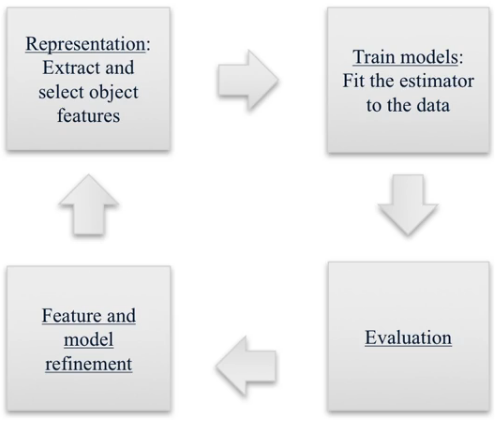
\includegraphics[width=\linewidth]{img/ML-cycle.png} 
\end{center}

You see that evaluation is a key part of this development cycle in applied machine learning. 

Once a model is trained, the evaluation step provides critical feedback on the trained model's performance characteristics. Particularly those that might be important for your application. 

The results of the evaluation step, for example, might help you understand which data instances are being classified or predicted incorrectly. Which might in turn suggest better features or different kernel function or other refinements to your learning model in the feature and model refinement phase. 

As we discussed earlier, the objective function that's optimized during the training phase may be a different, what's called \emph{a surrogate metric}. That's easier to use in practice for optimization purposes than what's used for the \emph{evaluation metric}. 

For example, a commercial search engine might use a ranking algorithm that is trained to recommend relevant web pages that best match a query. In other words, trying to predict a relevant label for a page. And that might be the objective in the \emph{training} phase. 

But there are many evaluation methods in the \emph{evaluation} phase that could be applied to measure aspects of that search engine's performance using that ranking algorithm, that are important to the search company's business, for example. Such as how many unique users the system sees per day. Or how long the typical user search session is and so on. 

So the \emph{evaluation measures} are the ones that in the end are used to select between different trained models or settings. 

Actually commercial search applications typically use a scorecard of multiple evaluation metrics to make important business decisions. Or development decisions about what models are chosen for use. 

So it's very important to choose evaluation methods that \emph{match} the goal of your application. 

For predicting the correct digit from a handwritten image, let's say, where each digit is equally likely, then accuracy may be a sufficient metric. 

However, there are other possible aspects of evaluation of model performance that are beyond average accuracy that may be critical to measure. For example, in a health application that uses a classifier to detect tumors in a medical image, we may want the classifier to error on the side of caution. And flag anything that even has a small chance of being cancerous. Even if it means sometimes incorrectly classifying healthy tissue as diseased. 

In this case, the classifier evaluation method would try to reduce what are called false negative predictions. 

We'll look at this in more detail shortly. 

More generally, your application goal might be based on very different metrics, such as user satisfaction, amount of revenue to your page, or increase in patient survival rates. 

So in the end, you'll be selecting the model or parameter settings that optimize those end evaluation metrics that are important to your goal. 

So in this module, we'll be focusing first on the widely used case of evaluating binary classification. And then we'll look at evaluation for the more general case of multi-class evaluation as well as regression. 

Before we start defining and using some evaluation metrics for binary classification, lets start by looking at example of why just looking at accuracy may not be enough to gain a good picture of what a classifier's doing. 

It'll also show us how knowing more about the types of errors a learning algorithm makes can help us get a better picture of a model's predictive performance. 

\subsection{Evaluation metrics for an imbalanced class}

First, let's consider the case where we have a binary classification task, where there are a lot of instances labeled with the negative class. But only a few instances that belong to the positive class. 

For example, we might see this scenario in online search or recommender systems. Where the system has to predict whether or not to display an advertisement or product suggestion. 

Or show a query suggestion or item on a page that's likely to be relevant given a user's query and what they clicked on in the past and so on. So those would be the positive examples. But of course there are many, many irrelevant items that are in the negative class that don't make sense to show a user. And so this is called an imbalanced class scenario. 

Another example might be datasets of credit card transactions. Where the vast majority of transactions are classified as normal and not fraud 

with a small minority of transactions that could be classified as fraudulent. 

These situations, which also apply to multi-class classification problems, involve datasets that have imbalanced classes. Imbalanced classes are very common in machine learning scenarios, so it's important to understand how to work with them. 

In particular, let's assume that we have an e-commerce application. Where for every 1,000 randomly sampled product items, one of them is relevant to a user's need and the other 999 are not relevant. 

So recall that accuracy computed over a set of instances is just the number of instances where the classifier's label prediction was correct divided by the total number of instances. 

Let's suppose you develop a classifier for predicting relevant e-commerce items. And after you've finished the development, you measure its accuracy on the test set to be 99.9\%. At first, that might seem to be amazingly good, right? That's incredibly close to perfect. 

But let's compare that to a dummy classifier that always just predicts the most likely class, namely, the not relevant class. In other words, no matter what the actual instance is, the dummy classifier will always predict that an item is not relevant. 

So if we have a test set that has 1,000 items, on average 999 of them will be not relevant anyway. So our dummy classifier will correctly predict the not relevant label for all of those 999 items. And so the accuracy of the dummy classifier is also going to be 99.9\%. So in reality our own classifier's performance isn't impressive at all. It's no better than just always predicting The majority class without even looking at the data. Let's take a look at another example of classification with imbalanced classes on a real dataset using our notebook. 

I'll start here using the digits dataset, which has images of handwritten digits labeled with ten classes, representing the digits zero through nine. 

As we can see by letting the dataset and then computing the count of instances in each class, using numpy's bin count method. There are roughly the same number of instances in each class. So this dataset has balanced classes. 

However with this digits dataset, now what we're going to do is create a new dataset with two imbalanced classes. By labelling all digits that are not the digit 1 as the negative class with label 0, and digits that are 1 as the positive class, label 1. So what I've done here is dump the first few entries from the original labels along with the new binary label, so you can see the imbalance visually. 

Now when we use bincount, we can see that there are about 1,600 negative examples, but only 182 positive examples. So indeed, we have a dataset that is class imbalanced. Or as expected almost exactly a nine to one ratio of negative to positive examples. 

Now let's create a train test partition on this imbalance set. And then train a support vector machine classifier with these binary labels using the radial basis function as a kernel. We get the accuracy using the score method, and we can see this is just over 90\%. Again at first glance, 90\% accuracy for a classifier seems pretty good. 

\subsection{A null accuracy baseline}

\subsubsection{With Dummy Classifier}

However, now let's create a Dummy Classifier that correctly reflect the class imbalance to see if 90\% really is that impressive. \texttt{scikit-learn} makes it easy to create a dummy classifier just by using the DummyClassifier class as shown here. 


{\scriptsize
\begin{verbatim}
from sklearn.dummy import DummyClassifier

# Negative class (0) is most frequent
dummy_majority=DummyClassifier(strategy='most_frequent')
dummy_majority.fit(X_train, y_train)
# Therefore the dummy 'most_frequent' classifier always 
# predicts class 0
y_dummy_predictions = dummy_majority.predict(X_test)
dummy_majority.score(X_test, y_test)
0.9044444444444445
\end{verbatim}
}

Dummy classifiers, again, are called that because they don't even look at the data to make a prediction. They simply use the strategy or rule of thumb that you instruct them to use, when creating them. In fact, when you create the classifier, you set the strategy argument to tell it what rule of thumb to use to make its predictions. So here, we set this to the most frequent strategy to predict the most frequent class. 

The DummyClassifier here is used just like a regular classifier. So to prepare it for prediction, we call the fit method on the \texttt{x_train} and \texttt{y_train} variables that hold the training set instances and labels. 

Now this DummyClassifier won't actually be looking at the individual data instances of those variables. But it does use the \texttt{y_train} variable to determine which class in the training data is most frequent. 

Finally, just like a regular classifier, we can call the predict method to make predictions on the test set. 

This example shows the output of the DummyClassifier's predictions. And as promised, you can see it's always predicting 0 or the negative class for every instance in the test set. 

Now we can call the usual score method to get the accuracy of the DummyClassifier's constant negative prediction. 

And we can see it's also 90\%, the same as our earlier support vector machine classifier with radio bases function kernel. 

So that support vector classifier was actually performing only very slightly better than the DummyClassifier. 

The dummy classifier provides what is called a null accuracy baseline. That is the accuracy that can be achieved by always picking the most frequent class. 

You should \emph{not} use a dummy classifier for real classification problems, but it does provide a useful sanity check in point of comparison. 

\subsubsection{Other Types of Dummy Classifiers}

There are other types of dummy classifiers that provide null base lines corresponding to other choices of the strategy parameter as shown here. 

\subsubsection*{Most frequent strategy}

Most frequent is the strategy we've just seen that always predicts the most frequent label. The stratified strategy, unlike the constant most frequent prediction is a random prediction that's based on the class distributions. For example, if the positive class occurs 90\% of the time in the training set. Then the stratified DummyClassifier will output the positive class label with 90\% probability. Otherwise, it will output the negative class label. 
This can help ensure that metrics that rely on having counts of both positive and negative class prediction outcomes can be computed. 

\subsubsection*{Uniform strategy}

The uniform strategy is another random prediction method that will generate class predictions uniformly at random. That is, all classes have an equal chance at being output as opposed to being weighed by their frequency in the training set. This strategy may be useful for gaining an accurate estimate of what the most common types of prediction errors for each class. 

\subsubsection*{Constant strategy}

The constant strategy can be useful when computing some metrics like F score, which we will cover in a few minutes. Well, why is that? Well, when we have a binary classification task where the most frequent class is the negative class. Turns out that using the most frequent strategy will never predict the positive class. And will never be able to count the number of positive instances that are correctly predicted. And so the overall count of such positive correct predictions will be 0. 

So this in turn as you will see in a few minutes, we'll cause some important metrics like \texttt{F scores} to always be zero. 

So using the constant strategy, we can force a dummy classifier to always predict the positive class even if it's the minority class in a set of classes. And this will lead to more meaningful computation of F-score. 

So what does it mean if we discover that our classifier has close to the DummyClassifier's performance? While typically it means that the features in our model may be ineffective, or erroneously computed or missing for some reason, it could also be caused by a poor choice of kernel or hyperparameter in the model. 

For example, if we change the support vector classifier's kernel parameter to \texttt{linear} from \texttt{rbf}. And recompute the accuracy on this retrain classifier, we can see that this leads to much better performance of almost 98\% compared to the most frequently class based line of 90\%. 

Finally, if you have accuracy that is close to that of a dummy classifier, it could be because there is indeed a large class \emph{imbalance}. And the accuracy gains produced by the classifier on the test set simply applied too few examples to produce a significant gain. 

In general, \textbf{for imbalanced} classification problems, you should use metrics \emph{other} than accuracy. We'll look at one shortly called AUC, which is short for area under the curve. 


\subsection{Binary Classification Outcomes}

Now let's look more carefully at the different types of outcomes we might see using a binary classifier. This will give us some insight into why using just accuracy doesn't give a complete picture of the classifier's performance. And will motivate our definition and exploration of additional evaluation metrics. 

With a positive and negative class, there are four possible outcomes that we can break into two cases corresponding to the first and second row of this matrix. 

If the true label for an instance is negative, the classifier can predict either negative, which is correct, and call the \textbf{true negative~--- TN}. Or it can erroneously predict positive, which is an error and called a \textbf{false positive~--- FP}. 

If the true label for an instance is positive, the classifier can predict either negative, which is an error and called a \textbf{false negative~--- FN}. Or it can predict positive, which is correct and that's called a \textbf{true positive~--- TP}. 

So maybe a quick way to remember this is that the first word in these matrix cells is false, if it's a a classifier error, or true if it's a classifier success. 

The second word is negative if the predicted label is negative and positive if the predicted label is positive. 

Another name for a false positive that you might know from statistics is a \textbf{type one error}. And another name for a false negative is a \textbf{type two error}. 

We'll also use capital \textbf{N} here to denote the total number of instances, of the sum of all the values in the matrix, the number of data points we're looking at. 

\begin{center}
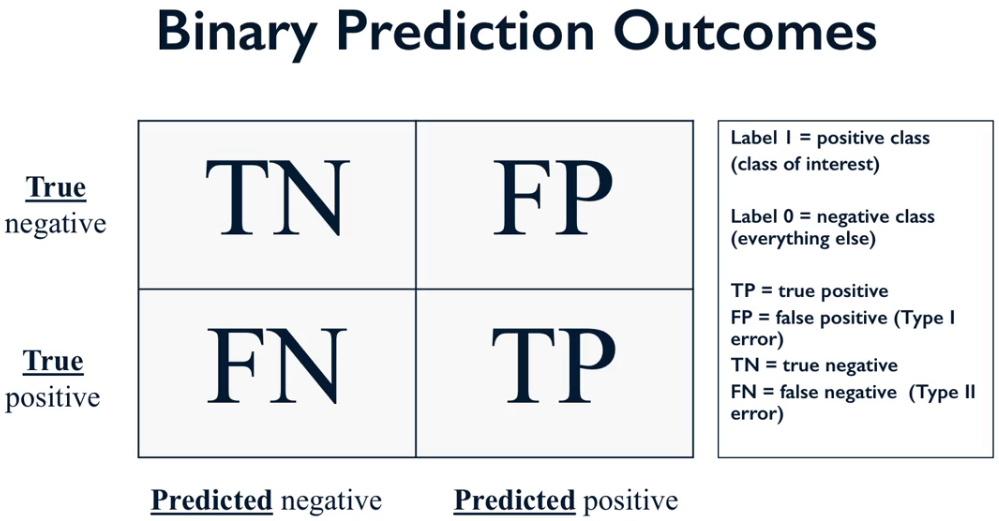
\includegraphics[width=\linewidth]{img/Binary-Prediction-Outcomes.png} 
\end{center}

This matrix of all combinations of predicted label and true label is called a \textbf{confusion matrix}. 

We can take any classifier prediction on a data instance and associate it with one of these matrix cells, depending on the true label of the instance and the classifier's predicted label. 

This also applies to multi-class classification, in addition to the special case of binary classification I've shown here. In the multi-class case with k classes, we simply have a k by k matrix instead of a two by two matrix. Scikit-learn makes it easy to compute a confusion matrix for your classifier. Let's take a look at the notebook. Here, we import the confusion matrix class from sklearn.metrics. We're going to use the same training set from the digits data set with the binary imbalance labels that we created earlier. 

To get the confusion matrix, we simply pass the \texttt{y_test} set of predicted labels and the y predicted set of predicted labels and then print the output. The order of the cells of the little matrix output here is the same as the one I just showed on the slide. 

True negative and false negative are in the first column, and true positive and false positive are in the second column. 

In particular, the successful predictions of the classifier are on the diagonal where the true class matches the predicted class. The cells off the diagonal represent errors of different types. 

Here, we compute the confusion matrices for different choices of classifier in the problem so we can see how they shift slightly with different choices of model. 

And this gives us some insight into the nature of successes and failures observed for each type of classifier. 

So first, we'll apply the most frequent class DummyClassifier we saw earlier. What we can see here is that the right column, that represent cases where the classifier predicted the positive class, is all zero. Which makes sense for this dummy classifier because it's always predicting the negative class, the most frequent one. We see that 407 instances are true negatives, and there are 43 errors that are false negatives. 

Here we apply the stratified DummyClassifier that gives random output in proportion to the ratio labels in the training set. Now the right column is no longer all zero because this DummyClassifier does predict occasionally predict the positive class. If we add the numbers in the right column, we see that 32 plus 6 equals 38 times the number of times the classifier predicted the positive class. Of those times, in six cases, the lower right diagonal, this was a true positive. 

In the next case, we'll apply a support vector classifier with linear kernel and seed parameter equal to one. 

We note that looking along the diagonal compared to the stratified dummy classifier above, which had a total of 375 plus 6, or 381 correct predictions. The support vector classifier has a total of 402 plus 38, which is 440 correct predictions on the same data set. 

Likewise, we can apply a logistic regression classifier, and that obtains similar results to the support vector classifier. And finally, we can apply a decision tree classifier, and look at the confusion matrix that results from that. One thing we notice is, that unlike the support vector or logistic regression classifier, which had balanced numbers of false negatives and false positives. The decision tree makes more than twice as many false negative errors, 17 of them actually, as false positive errors, of which there are 7. Now that we've seen how a confusion matrix can give us a little more information about the types of errors a classifier makes, we're ready to move ahead and and define some new types of evaluation metrics that use information from the computing matrix to give different perspectives on classifier performance.

\end{multicols}

\section{Confusion Matrices and Basic Evaluation Metrics}
\begin{multicols}{2}

So, let's go back to the matrix of possible binary classification outcomes. This time filled out with the actual counts from the notebooks decision tree output. Remember our original motivation for creating this matrix was to go beyond a single number accuracy, to get more insight into the different types of prediction successes and failures of a given classifier. Now we have these four numbers that we can examine and compare manually. 

Let's look at this classification result visually to help us connect these four numbers to a classifier's performance. 

\begin{center}
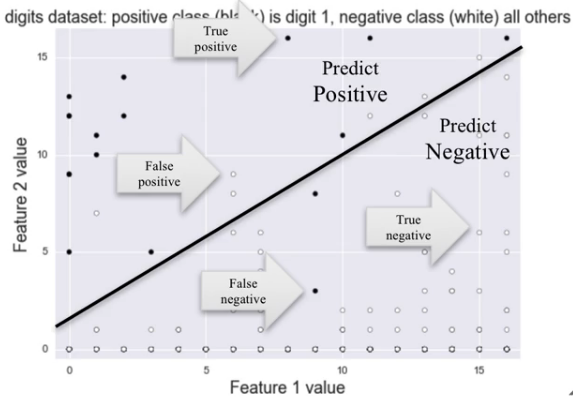
\includegraphics[width=\linewidth]{img/Diff-error-types-visualization.png} 
\end{center}

What I've done here is plot the data instances by using two specific feature values out of the total 64 feature values that make up each instance in the digits dataset. 

The black points here are the instances with true class positive namely the digit one and the white points have true class negative, that is, there are all the other digits except for one. The black line shows a hypothetical linear classifier's decision boundary for which any instance to the left of the decision boundary is predicted to be in the positive class and everything to the right of the decision boundary is predicted to be in the negative class. 

The true positive points are those black points in the positive prediction region and false positives are those white points in the positive prediction region. Likewise, true negatives are the white points in the negative prediction region and false negatives are black points in the negative prediction region. 

\subsection{Accuracy}

We've already seen one metric that can be derived from the confusion matrix counts namely \emph{Accuracy}. The successful predictions of the classifier, the ones where the predicted class matches the true class are along the \emph{diagonal} of the confusion matrix. 

$$Accuracy = \frac{TP + TN}{TP + TN + FP + FN}$$

\subsection{Classification Error}

But, let's look at some other evaluation metrics we can compute from these four numbers. Well, a very simple related number that's sometimes used is \emph{Classification Error}. Classification Error is equivalent to  one minus the accuracy.

$$Classification\ Error = \frac{FP + FN}{TP + TN + FP + FN}$$

$$Classification\ Error = 1 - Accuracy$$

\begin{center}
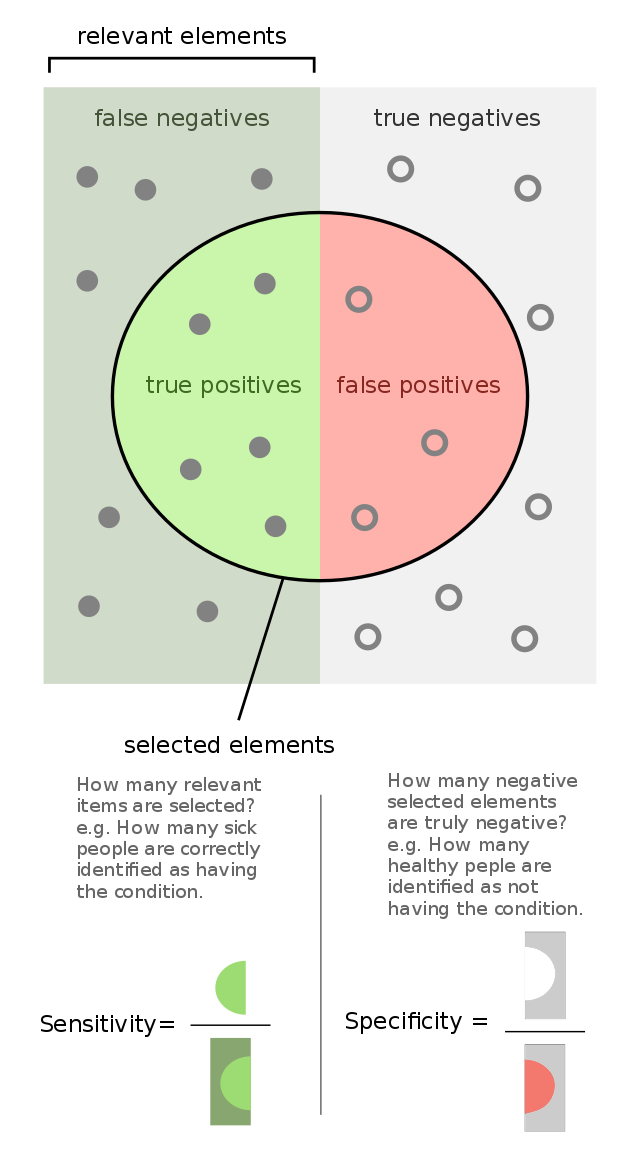
\includegraphics[width=\linewidth]{img/640px-Sensitivity-and-specificity.png} 
\end{center}

\subsection{Recall / True Positive Rate / Sensitivity}

Now, for a more interesting example, let's suppose, going back to our medical tumor detecting classifier that we wanted an evaluation metric that would give higher scores to classifiers that not only achieved the high number of \emph{true positives} but also \emph{avoided false negatives}. That is, that rarely failed to detect a true cancerous tumor. 

\emph{Recall}, also known as the \emph{True Positive Rate}, sensitivity or probability of detection~--- an evaluation metric. 

$$Recall = \frac{TP}{TP + FN}$$

What fraction of all positive instances does the classifier \emph{correctly} identify as positives?

You can see from this formula that there are two ways to get a larger recall number. First, by either increasing the number of true positives or by reducing the number of false negatives. Since this will make the denominator smaller. 

In this example there are 26 true positives and 17 false negatives which gives a recall of 0.6. 



\subsection{Precision}

Now suppose that we have a machine learning task, where it's really important to avoid false positives. In other words, we're fine with cases where not all true positive instances are detected but when the classifier does predict the positive class, we want to be very confident that it's correct. 

A lot of customer facing prediction problems are like this, for example, predicting when to show a user A query suggestion in a web search interface might be one such scenario. Users will often remember the failures of a machine learning prediction even when the majority of predictions are successes. 

So, precision is an evaluation metric that reflects the situation. 

$$Precision = \frac{TP}{TP + FP}$$

What fraction of positive predictions are correct?

So to increase precision, we must either increase the number of true positives the classifier predicts or reduce the number of errors where the classifier incorrectly predicts that a negative instance is in the positive class. 

Here, the classifier has made seven false positive errors and so the precision is 0.79. 

\subsection{False Positive Rate / Specificity}

Another related evaluation metric that will be useful is called the \emph{False Positive Rate}, also known as \emph{specificity}. This gives the fraction of all negative instances that the classifier incorrectly identifies as positive. 

$$False\ Positive\ Rate = \frac{TN}{TN + FP}$$

What fraction of all negative instances does the classifier \emph{incorrectly} identify as positives?

Here, we have seven false positives, which out of a total of 407 negative instances, gives a false positive rate of 0.02. 

Going back to our classifier visualization, let's look at how precision and recall can be interpreted. The numbers that are in the confusion matrix here are derived from this classification scenario. We can see that a precision of 0.68 means that about 68 percent of the points in the positive prediction region to the left of the decision boundary or 13 out of the 19 instances are correctly labeled as positive. A recall of 0.87 means, that of all true positive instances, so all black points in the figure, the positive prediction region has 'found about 87 percent of them' or 13 out of 15. 

If we wanted a classifier that was oriented towards higher levels of precision like in the search engine query suggestion task, we might want a decision boundary instead that look like this. Now, all the points in the positive prediction region seven out of seven are true positives, giving us a perfect precision of 1.0. 

\begin{center}
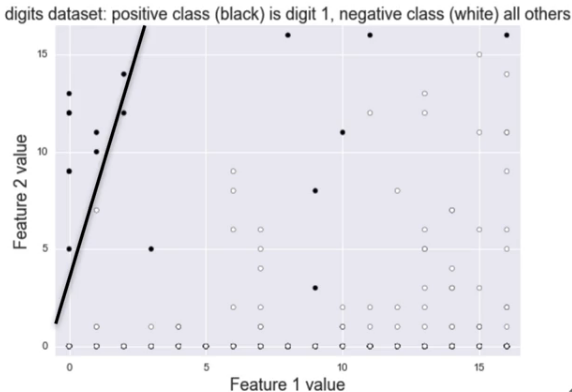
\includegraphics[width=\linewidth]{img/High-Precision-Lower-Recall.png} 
\end{center}

Now, this comes at a cost because out of the 15 total positive instances eight of them are now false negatives, in other words, they're incorrectly predicted as being negative. And so, recall drops to 7 divided by 15 or 0.47. 

On the other hand, if our classification task is like the tumor detection example, we want to minimize false negatives and obtain high recall. In which case, we would want the classifier's decision boundary to look more like this.

\begin{center}
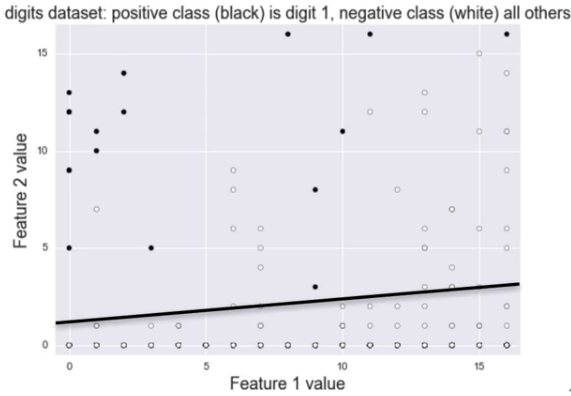
\includegraphics[width=\linewidth]{img/Low-Precision-High-Recall.png} 
\end{center}

 Now, all 15 positive instances have been correctly predicted as being in the positive class, which means these tumors have all been detected. 

However, this also comes with a cost since the number of false positives, things that the detector triggers as possible tumors for example that are actually not, has gone up. So, recall is a perfect 1.0 score but the precision has dropped to 15 out of 42 or 0.36. These examples illustrate a classic trade-off that often appears in machine learning applications. Namely, that you can often increase the precision of a classifier but the downside is that you may reduce recall, or you could increase the recall of a classifier at the cost of reducing precision. 

\emph{Recall oriented} machine learning tasks include medical and legal applications, where the consequences of not correctly identifying a positive example can be high. Often in these scenarios human experts are deployed to help filter out the false positives that almost inevitably increase with high recall applications. 

Many customer facing machine learning tasks, as I just mentioned, are often \emph{precision oriented} since here the consequences of false positives can be high, for example, hurting the customer's experience on a website by providing incorrect or unhelpful information. Examples include, search engine ranking and classifying documents to annotate them with topic tags. 

\subsection*{$F_1$ score and $F_\beta$ score}

When evaluating classifiers, it's often convenient to compute a quantity known as an $F_1$ score, that combines precision and recall into a single number. 

$$F_1 = 2 * \frac{Precision * Recall}{Precision + Recall}$$

$$F_1 = \frac{2*TP}{2*TP+FN+FP}$$

Mathematically, this is based on the harmonic mean of precision and recall using this formula. After a little bit of algebra, we can rewrite the $F_1$ score in terms of the quantities that we saw in the confusion matrix: true positives, false negatives and false positives. 

This $F_1$ score is a special case of a more general evaluation metric known as an $F_\beta$ score that introduces a parameter beta. 

$$F_\beta = (1+\beta^2) * \frac{Precision * Recall}{\beta^2*Precision + Recall}$$

$$F_\beta = \frac{(1+\beta^2)*TP}{(1+\beta^2)*TP+\beta * FN + FP}$$

By adjusting beta we can control how much emphasis an evaluation is given to precision versus recall. 

For example, if we have precision oriented users, we might say a beta equal to 0.5, since we want false positives to hurt performance more than false negatives. 

For recall oriented situations, we might set beta to a number larger than one, say two, to emphasize that false negatives should hurt performance more than false positives. 

The setting of beta equals one corresponds to the $F_1$ score special case that we just saw that weights precision and recall equally. 


\subsection{Metrics in Scikit-learn}

Let's take a look now at how we can compute these evaluation metrics in Python using scikit-learn. Scikit-learn provides functions \texttt{accuracy_score}, \texttt{precision_score}, \texttt{recall_score},  \texttt{f_score} and \texttt{fbeta_score}. The input to these functions is the same. The first argument \texttt{y_test} is the array of true labels of the test set data instances and the second argument is the array of predicted labels for the test set data instances. 

It's often useful when analyzing classifier performance to compute all of these metrics at once. So, sklearn metrics provides a handy \texttt{classification_report} function. Like the previous score functions, classification report takes the true and predicted labels as the first two required arguments. It also takes some optional arguments that control the format of the output. 

{\scriptsize
\begin{verbatim}
from sklearn.metrics import classification_report

print(classification_report(y_test, tree_predicted, 
      target_names=['not 1', '1']))
      
            precision recall f1-score support

       not 1     0.96   0.98     0.97     407
           1     0.79   0.60     0.68      43

   micro avg     0.95   0.95     0.95     450
   macro avg     0.87   0.79     0.83     450
weighted avg     0.94   0.95     0.94     450
\end{verbatim}
}

Here, we use the target names option to label the classes in the output table. The last column \texttt{support} shows the number of instances in the test set that have that true label. 

Here we show classification reports for four different classifiers on the binary digit classification problem. 
{\scriptsize
\begin{verbatim}
Random class-proportional (dummy)
               precision    recall  f1-score   support

       not 1       0.91      0.91      0.91       407
           1       0.12      0.12      0.12        43

   micro avg       0.83      0.83      0.83       450
   macro avg       0.51      0.51      0.51       450
weighted avg       0.83      0.83      0.83       450

SVM
               precision    recall  f1-score   support

       not 1       0.99      0.99      0.99       407
           1       0.88      0.88      0.88        43

   micro avg       0.98      0.98      0.98       450
   macro avg       0.94      0.94      0.94       450
weighted avg       0.98      0.98      0.98       450

Logistic regression
               precision    recall  f1-score   support

       not 1       0.99      0.99      0.99       407
           1       0.86      0.86      0.86        43

   micro avg       0.97      0.97      0.97       450
   macro avg       0.92      0.92      0.92       450
weighted avg       0.97      0.97      0.97       450

Decision tree
               precision    recall  f1-score   support

       not 1       0.96      0.98      0.97       407
           1       0.79      0.60      0.68        43

   micro avg       0.95      0.95      0.95       450
   macro avg       0.87      0.79      0.83       450
weighted avg       0.94      0.95      0.94       450
\end{verbatim}
}

The first set of results is from the dummy classifier and we can see that as expected both precision and recall for the positive class are very low since the dummy classifier is simply guessing randomly with low probability of predicting that positive class for the positive instances. 

\end{multicols}

\section{Classifier Decision Functions}
\begin{multicols}{2}

Many classifiers in scikit learn can provide information about the uncertainty associated with a particular prediction either by using the \textbf{decision function} method or the \textbf{predict proba} method. 

\subsection{Decision function method}

When given a set of test points, the decision function method provides for each one a classifier score value that indicates how confidently classifier predicts the positive class. So there will be large magnitude positive scores for those points, or it predicts a negative class, there'll be large magnitude negative scores for negative points. 

Here's an example in the notebook showing the first few instances from our classification problem using a logistic regression classifier. We can see the instances in the negative class often have large magnitude negative scores. And indeed the instances in the positive class has positive scores from the logistic regression classifier. 

\subsection{Predict proba function}

Likewise, the \texttt{predict_proba} function provides \emph{predicted probabilities} of class membership. 

Typically a classifier would choose the more likely class. That is in a binary classifier, the class with probability greater than 50\%. 

\subsection{Decision threshold}

Adjusting this decision threshold affects the prediction of the classifier. A higher threshold means that a classifier has to be more confident in predicting the class. For example, we might predict class one only if the estimated probability of class one was over 70\%. And this results in a more conservative classifier. 

Here's an example of getting these prediction probabilities for the test instances for the same logistic regression classifier. 

You can see that many entries with a positive label of one, have a high probability like 0.995. While many negative label instances have a very low prediction probability. 

\textbf{Note} that \emph{not all} models provide useful probability estimates of this type. For example, a model that was over-fit to a trending set, might provide overly optimistic high probabilities that were in fact not accurate. 

Now, we can use these decision scores or prediction probabilities for getting more complete evaluation picture of a classifiers performance. For a particular application, we might pick a specific decision threshold depending on whether we want the classifier to be more or less conservative about making false-positive or false-negative errors. 

It might not be entirely clear when developing a new model, what the right decision threshold would be, and how that choice will affect evaluation metrics like precision and recall. So instead, what we'll do is, look at how classifier performs for all possible decision thresholds. 

This example shows how that works. On the left here is a list of test instances with their true label and classifier score. 

\begin{center}
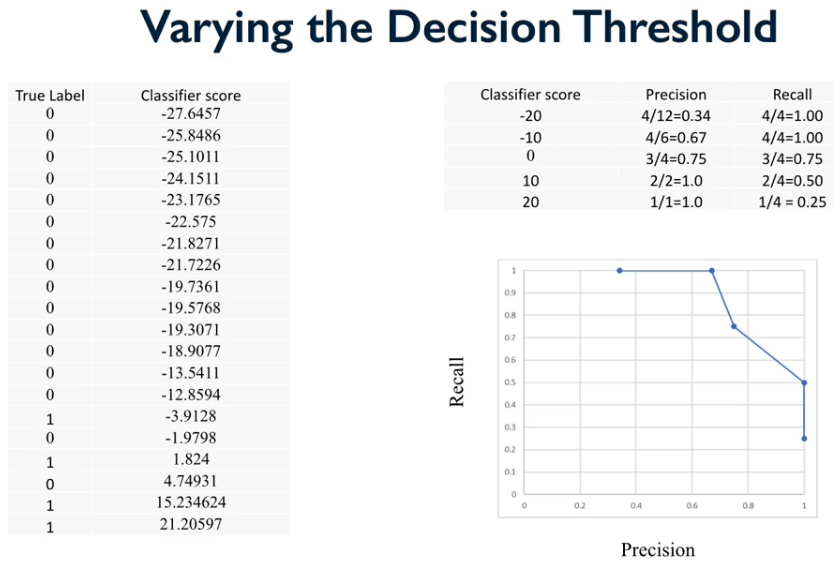
\includegraphics[width=\linewidth]{img/Varying-Decision-Threshold.png} 
\end{center}

If we set a decision threshold, then all the instances above that line, for example if we set the decision threshold to be -20 here. 

Then, all the instances above the line are below the threshold of -20. So -20 or less and all the instances in this direction are above the threshold of -20. And so the ones below the threshold will be predicted to be in the- class. 

And the ones above the threshold will be predicted to be in the + class. 

So, if we pick the specific threshold, so in this case, -20. And we partition the test points in this way. We can compute partition and recall for the points that are predicted to be in the positive class. So in this case, we have 12 instances here, 12 total instances. 

They're being predicted as positive and only four of them, this one, this one, this one, and this one are actually positive and so the precision here is 4 divided by 12 or approximately 0.34. 

The recall on the other hand, there are four positive labeled instances in the whole set of test examples here and we've found all of them with this particular threshold setting. So the recall here is 4 out of 4, we found all four positive labeled examples. And so, for this particular threshold of -20, we can obtain precision on re cost score for that threshold. 

Let's pick a different threshold let's look at what happened when the threshold is -10? Right here, so again anything below this line is treated and has a higher value than -10 here, so those would be treated as + predictions. 

Things above the line have a score below -10, so these would be predicted to be 

And again, we can compute a precision and recall for this decision threshold setting, and we can see here that there are a total of six instances in the + prediction class. Of which four are actually of the positive class, and so the precision here is 4 over 6 or about 0.67. And again, the recall here is going to be 4 out of 4, and it's going to be 1.0. Again, so that corresponds to this point in the table over here. And then as were computing these different precision and recalls for different Thresholds. We can also plot them on this precision recall chart. So the first pair of precision recall numbers that I got, 0.34 and 1.0, we can plot on this point in precision recall space. The second example, so this was for the threshold of -20. 

When the threshold was -10, we got precision of .67 and a recall of 1 corresponding to this point that we can plot. 

And so you can see that if we do this for a number of other thresholds, for example the threshold of 0, we'll get a precision of 0.75. And a recall of 0.75 that corresponds to this point. 

And in that choice of decision threshold. And we can keep doing that for different thresholds. And we actually are plotting a series of points through the space which we can be connected at as a curve. 

And so in this way, we can get a more complete picture by varying the threshold of how the precision and recall of the result and classifier output changes as a function of the decision threshold. 

And this resulting chart here is called a precision recall curve and we'll look at it in more detail next. 

\end{multicols}

\section{Precision-Recall and ROC curves}
\begin{multicols}{2}

\subsection{Precision-Recall Curves}

Precision-Recall Curves are very widely used evaluation method from machine learning. 

As we just saw in example, the x axis shows precision and the y axis shows recall. 

Now an ideal classifier would be able to achieve perfect precision of 1.0 and perfect recall of 1.0. So the optimal point would be up here in the top right. And in general, with precision recall curves, the closer in some sense, the curve is to the top right corner, the more preferable it is, the more beneficial the tradeoff it gives between precision and recall. And we saw some examples already of how there is a tradeoff between those two quantities, between precision and recall, with many classifiers. 


\begin{center}
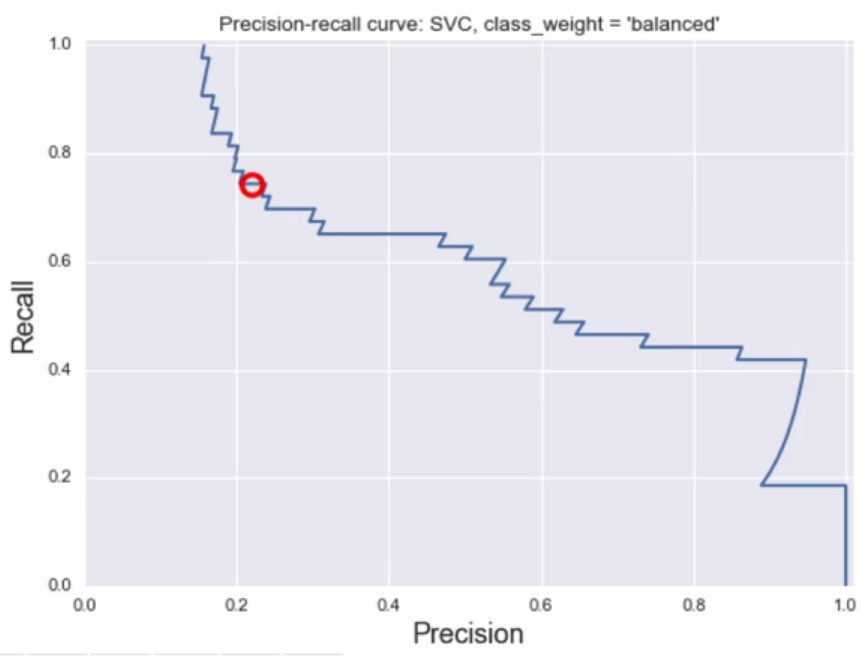
\includegraphics[width=\linewidth]{img/Precision-Recall-curve.png} 
\end{center}

This example here is an actual precision recall curve that we generated using the following notebook code. 

{\scriptsize
\begin{verbatim}
from sklearn.metrics import precision_recall_curve

precision, recall, thresholds = 
    precision_recall_curve(y_test, y_scores_lr)
closest_zero = np.argmin(np.abs(thresholds))
closest_zero_p = precision[closest_zero]
closest_zero_r = recall[closest_zero]

plt.figure()
plt.xlim([0.0, 1.01])
plt.ylim([0.0, 1.01])
plt.plot(precision, recall, label='Precision-Recall Curve')
plt.plot(closest_zero_p, closest_zero_r, 'o', 
    markersize = 12, fillstyle = 'none', c='r', mew=3)
plt.xlabel('Precision', fontsize=16)
plt.ylabel('Recall', fontsize=16)
plt.axes().set_aspect('equal')
plt.show()
\end{verbatim}
}
The red circle indicates the precision and recall that's achieved when the decision threshold is zero. So I created this curve using exactly the same method as we saw in the previous example, by looking at the decision function output from a support vector classifier. Applying varying  decision boundary, looking at how the precision of recall change as the decision boundary changed. Fortunately, scikit-learn has a function that's built in that does all of that, that can compute the precision- recall curve. 

So you can see that in this particular application there is a general downward trend. So as the precision of the classifier goes up, the recall tends to go down. 

In this particular case you'll see also that it's not exactly a smooth curve. There are some jaggy areas and, in fact, the jumps tend to get a little bigger as we approach maximum precision. This is a consequence of how the formulas for precision and recall are computed. They use discrete counts that include the number of true positives. And so as the decision threshold increases, there are fewer and fewer points that remain as positive predictions. So the fractions that are computed for these smaller numbers can change pretty dramatically with small changes in the decision threshold. And that's why these sort of trailing edges of the precision-recall curve can appear a bit jagged when you plot them. 

\subsection{Receiver Operating Characteristic (ROC) curves}

ROC curves or receiver operating characteristic curves are a very widely used visualization method that illustrate the performance of a binary classifier. 

\begin{center}
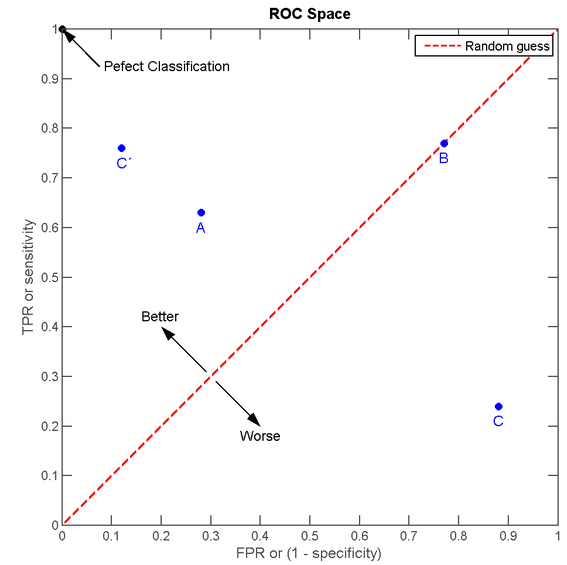
\includegraphics[width=\linewidth]{img/640px-ROC-space-2.png} 
\end{center}



ROC curves on the X-axis show a classifier's False Positive Rate so that would go from 0 to 1.0, and on the Y-axis they show a classifier's True Positive Rate so that will also go from 0 to 1.0. The ideal point in ROC space is one where the classifier achieves zero, a false positive rate of zero, and a true positive rate of one. So that would be the upper left corner. 

So curves in ROC space represent different tradeoffs as the decision boundary, the decision threshold is varied for the classifier. So just as in the precision recall case, as we vary decision threshold, we'll get different numbers of false positives and true positives that we can plot on a chart. 


\begin{center}
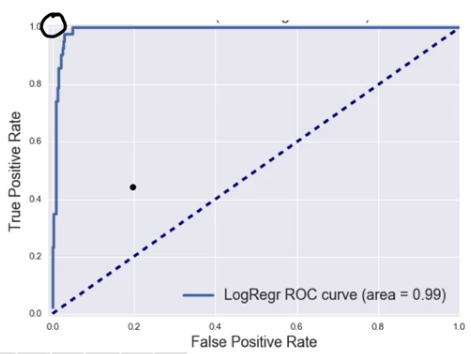
\includegraphics[width=\linewidth]{img/ROC-curve.png} 
\end{center}

The dotted line here that I'm showing is the classifier curve that secretly results from a classifier that randomly guesses the label for a binary class. 

It's basically like flipping a coin. If you have two classes with equal numbers of positive and negative incidences, then flipping a coin will get you randomly equal numbers of false positives and true positives for a large virus data sets. So the dotted line here is used as a base line. So bad classifier will have performance that is random or maybe even worse than random or be slightly better than random. Reasonably good classifier will give an ROC curve that is consistently better than random across all decision threshold choices. 

And then an excellent classifier would be one like I've shown here, which is way up into the left. 

This particular example is an example of a logistic regression classifier using the notebook example you've seen. 

So, the shape of the curve can be important as well, the steepness of the curve, we want classifiers that maximize the true positive rate while minimizing the false positive rate. 

Now as we'll see next, we can qualify the goodness of a classifier in some sense by looking at how much area there is underneath the curve. 

So the area underneath the random classifier is going to be 0.5 but then the area, as you can see, the size of the bumpiness of the classifier as it approaches the top left corner. Well, the area underneath the curve will get larger and larger. It will approach 1. And so, as we'll see in the next slide. 

\subsection{Area Under the ROC Curve (AUC)}

We use something called area under the curve, AUC. That's the single number that measures this total area underneath the ROC curve as a way to summarize a classifier's performance. So, an AUC of zero represents a very bad classifier, and an AUC of one will represent an optimal classifier. In \texttt{Scikit-learn} it is the \texttt{roc_auc_score()}.

\end{multicols}

\section{Multi-Class Evaluation}
\begin{multicols}{2}

Now that we've looked at evaluation of binary classifiers, let's take a look at how the more general case of multi class classification is handled in evaluation. So in may respects, multi-class evaluation is a straightforward extension of the methods we use in binary evaluation. Instead of two classes, we have multiple classes. So, the results for multi-class evaluation amount to a collection of true verses predicted binary outcome per class. And just as we saw in the binary case, you can generate confusion matrices in the multi-class case. They're especially useful when you have multiple classes, because there are many different kinds of errors that result from one true class being predicted as a different class. We'll look at an example of that. Classification reports that we saw in the binary case are easy to generate for the multi-class case. Now the one area, which is worth a little more examination is how averaging across classes takes place. 

There are different ways to average multi-class results that we'll cover shortly. And the support, the number of instances for each class is important to consider. So just as we're all interested in how to handle imbalance classes in the binary case, it's important as you will see to consider similar issues of how the support for classes might vary to a large or small extent across multiple classes. There is a case of multi-label classification in which each instance could have multiple labels. For example, a web page might be labeled with different topics that come from a predefined set of areas of interest. We won't cover multi-label classification in this lecture. Instead, we'll focus exclusively on multi-class evaluation. The multi-class confusion matrix is a straightforward extension of the binary classifier two by two confusion matrix. 

For example, in our digits data set, there are ten classes for the digits, zero through nine. So, the ten class confusion matrix is a ten by ten matrix with the true digit class indexed by row and the predicted digit class indexed by column. 

As with the two by two case, the correct prediction is by the classifier where the true class matches the predicted class are all along the diagonal and misclassifications are off the diagonal. 

In this example which was created using the following notebook code 

based on a support vector classifier with linear kernel, we can see that most of the predictions are correct with only a few misclassifications here and there. 

The most frequent type of mistake here is apparently misclassifying the true digit, eight as a predicted digit one which happened three times. 

And indeed, the overall accuracy is high, about 97\% as shown here. As an aside, it's sometimes useful to display a confusion matrix as a heat map in order to highlight the relative frequencies of different types of errors. So, I've included the code to generate that here. For comparison, I've also included a second confusion matrix on the same dataset for another support vector classifier that does much worse in a distinctive way. The only change is to use an RBF, radial basis function kernel instead of a linear kernel. 

While we can see for the accuracy number were about 43\% below the confusion matrix that the classifier is doing much worse than the delinear kernel, that single number doesn't give much insight into why. 

Looking at the confusion matrix, however, reveals that for every true digit class, a significant fraction of outcomes are to predict the digit four. That's rather surprising. For example, of the 44 instances of the true digit 2 in row 2, 17 are classified correctly, but 27 are classified as the digit 4. Clearly, something is broken with this model and I picked this second example just to show an extreme example of what you might see when things go quite wrong. This digits dataset is well-established and free of problems. But especially when developing with a new dataset, seeing patterns like this in a confusion matrix could give you valuable clues about possible problems, say in the feature pre-processing for example. So as a general rule of thumb as part of model evaluation, I suggest always looking at the confusion matrix for your classifier. To get some insight into what kind of errors it is making for each class including whether some classes are much more prone to certain kinds of errors than others. 

Next, just as in the binary case, you can get a classification report that summarizes multiple evaluation metrics for a multi-class classifier with an average metric computed for each class. 

Now what I'm about to describe, also applies to the binary class case, but it's easier to see when looking at multi-class classification problem with several classes. 

So, here's an example of how to compute macro-average precision and micro-average precision on a sample dataset that I have extracted from our fruit dataset. In this example, we have three columns where the first column is the true class of an example. The second column is the predictive class from some classifier and the third column is a binary variable that denotes whether the predictive class matches the two class. 

And here, we have in our, this is a multi-class classification problem. 

And so, we have three classes here. We have several instances there, the orange class. We have two instances that are the lemon class and we have two instances that are the apple class. 

So in this first example, we'll compute macro-average precision and the key aspect of macro-average precision is that each class has equal weight. So in this case, each of these classes will contribute one-third weight towards the final macro-average precision value. 

So, there are two steps to compute macro-average precision. The first one is to compute the metric. So in this case, we're going to compute precision within each class. So, let's take a look at the orange class. There are five total examples in the orange class and only one of them was predicted correctly by the classifier. And so, that leads to a precision for the orange class of 1 out of 5 or 0.20. For the second class, the lemon class. There are a total of two instances and only one of them was predicted correctly, and that leads to a precision of one-half or 0.50 for the lemon class. Let's write the precision for each of the classes that we have calculated. 


This was 0.5. 

And for the third class, the apple class. The classifier predicted both of these correctly. So, that's a precision of 2 out of 2 or 1.0. 

That's the first step. We've computed the precision metric within each class. And then in the second step, we simply average across these three to produce the final result, to get our final macro-average precision. And so we can simply compute the average of 0.2, 0.5 and 1 and we get our final macro-average precision for this set of results of 0.57. You'll notice here that no matter how many instances they were in each class, because we computed position within each class first, each class contributes equally to the overall macro-average. So we could have had, for example, a million examples and from the orange class. But that class would have still been weighted equally, because we would have first computed precision for the million orange examples and then that number would still get a third of the weight compared to the other two classes. So, that's macro-average precision. 

Micro-average precision is computed a little differently and it gives each instance in the data results here equal weight. In micro-average precision, we don't compute precision for each class separately. We treat the entire dataset, the entire set of results here as an aggregate outcome. So to compute micro-average precision, we simply look at how many of all the examples. We have nine examples here in total and micro-average precision will simply compute the precision for all the examples, regardless of class in the set of results. So out of these nine instances, we have found that the classifier predicted four of them correctly. 

And so, the micro-average precision is simply computed as 4/9 or 0.44. And you'll notice here that if we had a million instances of the orange class, for example, that with micro-average precision, because each instance has equal weight. That would lead to the orange class contributing many, many more instances to our overall micro-average precision. And so, the effect of micro-average precision is to give classes with a lot more instances much more influence. So, the average here would have been influenced much more by the million orange examples than by the two lemon and apple examples. 

And so, that is the difference between micro and macro-average precision. If the classes have about the same number of instances, macro and micro-average will be about the same. If some classes are much larger, have more instances than others and you want to weight your metric toward the largest ones, use micro-averaging. If you want to weight your metric towards the smallest classes, use macro-averaging. If the micro-average is much lower than the macro-average, then examine the larger classes for poor metric performance. If the macro-average is much lower than the micro-average, then you should examine the smaller classes to see why they have poor metric performance. Here, we use the average parameter on the scoring function. In the first example, we used the precision metric and specify whether we want micro-average precision which is the first case or macro-average precision in the second case. 

In the second example, we use the F1 metric and compute micro and macro-averaged F1. 

Now that we've seen how to compute these metrics, let's take a look at how to use them to do model selection. 

\end{multicols}

\section{Regression Evaluation}
\begin{multicols}{2}

We saw that for classification, because there were some scenarios like medical diagnostics predictions or costumer facing web site features, where the consequences of false positive were very different than false negatives. It made sense to distinguish these types of errors and do a more detailed analysis. In evaluating classifiers for example we looked at plots like precision recall curves that could show the trade offs a classifier could achieve between making errors of those two types. 

In theory, we could apply the same type of error analysis and more detailed evaluation to regression that we applied for classification. 

For example, we could analyze the regression model's predictions, and categorize errors of one type. Where the regression model's predicted value was much larger than the target value. Compared to a second error type, where the predicted value was much smaller than the target value. 

In practice though it turns out that for most applications of regression, distinguishing between these types of different errors is not as important. 
This simplifies evaluation for regression quite a bit. 

\subsection{$R^2$ score}

In most cases, the default $R^2$ score that's available for regression and psychic learn and that summarizes how well future instances will be predicted. It's adequate for most tasks. 

As a reminder, the $R^2$ score for \emph{perfect predictor} is \textbf{1.0}. And for a predictor that always output the \emph{same constant value}, the $R^2$ score is \textbf{0.0}. 

The $R^2$ score despite the squared in the name that suggests it's always positive does have the potential to go \emph{negative} for bad model fits, such as when fitting non-linear functions to data. 

\subsection{Alternative metrics}

There are a few alternative regression evaluation metrics you should be aware of that work differently than the $R^2$ score. 

\subsubsection{Mean absolute error}

Mean absolute error takes the mean absolute difference between the target and predicted values. In machine running terms this corresponds to the expected value of L1 norm laws. This is sometimes used for example to asses focused outcomes for regression in time series analysis. 

\subsubsection{Mean squared  error}
Mean squared error takes the mean squared difference between the target and predicted values and this corresponds to the expected value of the L2 norm loss. This is widely used for many regression problems and larger errors have correspondingly larger squared contributions to the mean error. 

Like mean absolute error, mean squared error doesn't distinguish between over and under estimates. 

\subsubsection{Median absolute error}

Finally one situation that does arise quite often, is the existence of \emph{outliers} in the data, which can have unwanted influence on the overall $R^2$ or mean squared value. So in those cases, when ignoring outlier is important, you can use the \emph{median} absolute error score, which is robust with the presence of outliers because it uses the median of the error distribution rather than the mean. 

\subsection{Dummy Regressors}

We saw how using how dummy classifiers could give us simple but useful baselines to compared against when evaluating a classifier. The same functionality exist for regression. 

DummyRegressors, as you might guess, are the counterpart to DummyClassifiers for regression. And they serve a similar role as a null outcome baseline and sanity check for regression models. Since regression models have continuous value prediction outputs. The strategy parameter for DummyRegressors gives you a choice of function that you can apply to the distribution of target values found in the training set. You can ask for the mean or median value of the training set targets. The value corresponding to the quantile that you provide or a custom constant value. 

There's a dummy regressor class that provides predictions using simple strategies that do not look at the input data.
 
\begin{center}
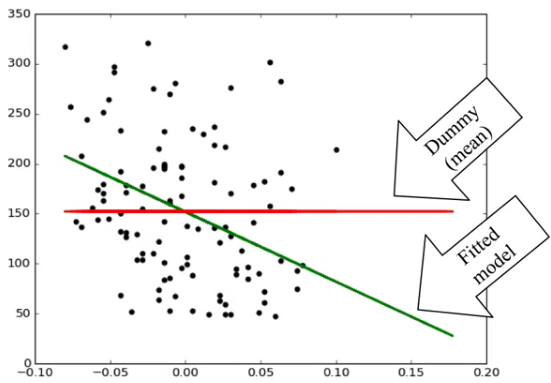
\includegraphics[width=\linewidth]{img/Dummy-Regressor.png}
\end{center}

This example which is available as the regression example from this lecture's notebook shows a scatter plot using database on a single input variable, which is plotted along the x axis from the diabetes data set. 

The points are the data instances from the test split and form a cloud that looks like it may trend down slightly to the right. 

The green line, which is also labeled fitted model is the default linear regression that was fit to the training points. We can see that it’s not a particularly strong fit to the test data. 

The red line labeled dummy mean, shows a linear model that uses the strategy of always predicting the mean of the training data. 

So this is an example of a dummy regressor. 

You can look at the notebook to see that a dummy regressor is created and used just like a regular regression model. You create, fit with the training data, and then call predict on the test data. Although again, like the dummy classifier you \emph{should not} use the dummy regressor for actual problems. Its only use is to provide a baseline for comparison. 

Looking at the regression metrics output from the linear model compared to the dummy model. 

\begin{verbatim}
Linear model, coefficients:[-698.80206267]
Mean squared error (dummy): 4965.13
Mean squared error (linear model): 4646.74
r2_score (dummy): -0.00
r2_score (linear model): 0.06
\end{verbatim}

We can see that as expected the dummy regressor achieves an $R^2$ score of \textbf{0}. Since it always makes a constant prediction without looking at the output. 

In this instance the linear model provides only slightly better fit than the dummy regressor, according to both mean squared error and the $R^2$ score. 

Aside from the strategy of always predicting the mean of the training target values, you could also create some other flavors of dummy regressors that always predict the \emph{median} of the training target values, or a particular \emph{quantile} of those values, or a specific custom \emph{constant value} that you provide. 

Although regression typically has simpler evaluation needs than classification, it does pay to double check to make sure the evaluation metric you choose for a regression problem does penalize errors in a way that reflects the consequences of those errors for the business, organizational, or user needs of your application. 

\end{multicols}

\section{Model Selection: Optimizing Classifiers for Different Evaluation Metrics}
\begin{multicols}{2}

Now that you've seen a number of different evaluation metrics for both binary and multiclass classification, let's take a look at how you can apply them as criteria for selecting the best classifier for your application, otherwise known as \emph{model selection}. 

In previous lectures we've seen a number of different evaluation frameworks for potential model selection. 

First, we simply did \emph{training and testing on the same dataset}, which as we well know, typically overfits badly and doesn't generalize well to new data. As a side note however, it can serve as a \emph{useful sanity check} to make sure your software engineering and feature generation pipeline is working correctly. 

Second, we frequently use the \emph{train-test split} to produce a single evaluation metric. While fast and easy, this doesn't give as realistic a set of estimates for how well the model may work on future new data. And we don't get a good picture for the variance in the evaluation metrics that may result as we do prediction on different test sets. 

Third, we used \emph{k-fold cross-validation} to create K random train-test splits, where the evaluation metric was averaged across splits. This leads to models that are more reliable on unseen data. 

In particular, we can also use grid search using for example the \texttt{GridSearchCV} method within each cross-validation fold, to find optimal parameters for a model with respect to the evaluation metric.

The default evaluation metric used for a cross-validation score or GridSearchCV is \emph{accuracy}. So how do you apply the new metrics you've learned about here like AUC in model selection? Scikit-learn makes this very easy. You simply add a \texttt{scoring} parameter that's set to the string with the name of the evaluation metric you want to use. 

\subsection{Cross Validation}

Here we're running five folds using a support vector classifier with a linear kernel and C parameter set to one. 

{\scriptsize
\begin{verbatim}
from sklearn.model_selection import cross_val_score
from sklearn.svm import SVC

dataset = load_digits()
# again, making this a binary problem with 'digit 1' 
# as positive class and 'not 1' as negative class
X, y = dataset.data, dataset.target == 1
clf = SVC(kernel='linear', C=1)

# accuracy is the default scoring metric
print('Cross-validation (accuracy)', 
       cross_val_score(clf, X, y, cv=5))
# use AUC as scoring metric
print('Cross-validation (AUC)', 
 cross_val_score(clf, X, y, cv=5, scoring = 'roc_auc'))
# use recall as scoring metric
print('Cross-validation (recall)', 
  cross_val_score(clf, X, y, cv=5, scoring = 'recall'))

Cross-validation (accuracy) 
[0.91944444 0.98611111 0.97214485 0.97493036 0.96935933]
Cross-validation (AUC) 
[0.9641871  0.9976571  0.99372205 0.99699002 0.98675611]
Cross-validation (recall) 
[0.81081081 0.89189189 0.83333333 0.83333333 0.83333333]
\end{verbatim}
}

The first call to cross-val score just uses default \texttt{accuracy} as the evaluation metric. The second call uses the scoring parameter using the string '\texttt{roc_auc}', and this will use AUC as the evaluation metric. The third call sets the scoring parameter to '\texttt{recall}', to use that as the evaluation metric. You can see the resulting list of five evaluation values, one per fold for each metric. 

Now, here we're not doing any parameter tuning we're simply evaluating our model's average performance across multiple folds. 

\subsection{Grid Search}

Now, in this grid search example we use a support vector classifier that uses a \texttt{rbf}~--- radius base function kernel. And the \emph{critical} parameter here is the \texttt{gamma} parameter that intuitively sets the radius or width of influence of the kernel. We use \texttt{GridSearchCV} to find the value of \texttt{gamma} that optimizes a given evaluation metric in two cases. 

{\tiny
\begin{verbatim}
from sklearn.svm import SVC
from sklearn.model_selection import GridSearchCV
from sklearn.metrics import roc_auc_score

dataset = load_digits()
X, y = dataset.data, dataset.target == 1
X_train, X_test, y_train, y_test = train_test_split(X, y, random_state=0)

clf = SVC(kernel='rbf')
grid_values = {'gamma': [0.001, 0.01, 0.05, 0.1, 1, 10, 100]}

# default metric to optimize over grid parameters: accuracy
grid_clf_acc = GridSearchCV(clf, param_grid = grid_values)
grid_clf_acc.fit(X_train, y_train)
y_decision_fn_scores_acc = grid_clf_acc.decision_function(X_test) 

print('Grid best parameter (max. accuracy): ', grid_clf_acc.best_params_)
print('Grid best score (accuracy): ', grid_clf_acc.best_score_)

# alternative metric to optimize over grid parameters: AUC
grid_clf_auc = GridSearchCV(clf, param_grid = grid_values, 
                            scoring = 'roc_auc')
grid_clf_auc.fit(X_train, y_train)
y_decision_fn_scores_auc = grid_clf_auc.decision_function(X_test) 

print('Test set AUC: ', roc_auc_score(y_test, y_decision_fn_scores_auc))
print('Grid best parameter (max. AUC): ', grid_clf_auc.best_params_)
print('Grid best score (AUC): ', grid_clf_auc.best_score_)

Grid best parameter (max. accuracy):  {'gamma': 0.001}
Grid best score (accuracy):  0.9962880475129918

Test set AUC:  0.99982858122393
Grid best parameter (max. AUC):  {'gamma': 0.001}
Grid best score (AUC):  0.9998741278302142
\end{verbatim}
}

In the first case, we just optimize for average accuracy; in the second case we optimize for AUC. In this particular case the optimal value of gamma happens to be the same, point zero-zero-one, for both evaluation metrics. As we'll see later in other cases, the optimal parameter value can be quite different depending on the evaluation metric used to optimize. 

You can see the complete list of names for the evaluation metric supported by the scoring parameter by running the following code that uses the \texttt{scores} variable imported from sklearn metrics. 

{\scriptsize
\begin{verbatim}
from sklearn.metrics.scorer import SCORERS
print(sorted(list(SCORERS.keys())))

['accuracy', 'adjusted_mutual_info_score', 
'adjusted_rand_score', 'average_precision', 
'balanced_accuracy', 'brier_score_loss', 
'completeness_score', 'explained_variance', 'f1', 
'f1_macro', 'f1_micro', 'f1_samples', 'f1_weighted',
'fowlkes_mallows_score', 'homogeneity_score', 
'mutual_info_score', 'neg_log_loss', 
'neg_mean_absolute_error', 'neg_mean_squared_error',
'neg_mean_squared_log_error', 'neg_median_absolute_error', 
'normalized_mutual_info_score', 'precision', 
'precision_macro', 'precision_micro', 'precision_samples',
'precision_weighted', 'r2', 'recall', 'recall_macro', 
'recall_micro', 'recall_samples', 'recall_weighted', 
'roc_auc', 'v_measure_score']
\end{verbatim}
}

You can see metrics for classification such as the string \texttt{'precision_micro'} that represents micro-averaged precision as well as metrics for regression such as the $R^2$ metric for $R^2$ regression loss. 

Let's take a look at a specific example that shows how a classifier's decision boundary changes when it's optimized for different evaluation metrics. This classification problem is based on the same binary digit classifier training and test sets we've been using as an example throughout the notebook. 

\begin{center}
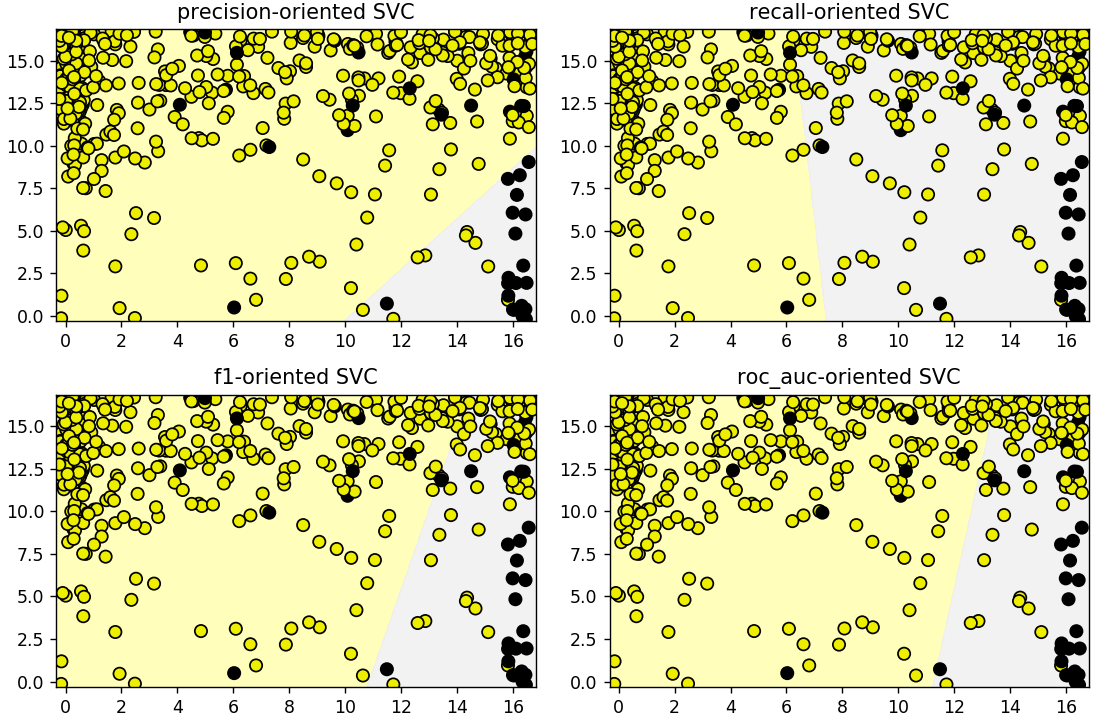
\includegraphics[width=\linewidth]{img/Optimizing-Classifier.png} 
\end{center}


In these classification visualization examples, the positive examples, the digit one are shown as black points and the region of positive class prediction is shown in the light-colored or yellow region to the right of this decision boundary. The negative examples, all other digits, are shown as white points. And the region of negative class prediction here in these figures is to the left of the decision boundary. The data points have been plotted using two out of the 64 future values in the digits' dataset and have been jittered a little. That is, I've added a little bit of random noise so we can see more easily the density of examples in the feature space. 

Here's the scikit-learn code that produced this figure. We apply grid search here to explore different values of the optional class weight parameter that controls how much weight is given to each of the two classes during training. As it turns out, optimizing for different evaluation metrics results in different optimal values of the class weight parameter. As the class weight parameter increases, more emphasis will be given to correctly classifying the positive class instances. 

%\begin{center}
%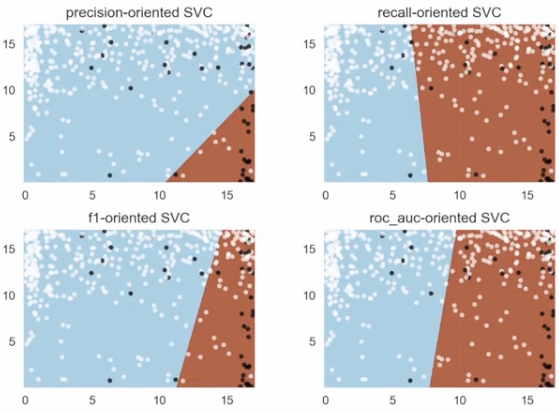
\includegraphics[width=\linewidth]{img/Optimizing-Classifier2.png} 
%\end{center}

The precision-oriented classifier we see here with class weight of two, tries hard to reduce false negatives while increasing true positives. So it focuses on the cluster of positive class points in the lower right corner where there are relatively few negative class points. Here, precision is over 50 percent. 

In contrast, the recall-oriented classifier with class weight of 50, tries hard to reduce the number of false negatives while increasing true positives. That is, it tries to find most of the positive class points as part of its positive class predictions. We can also see that the decision boundary for the F1-oriented classifier has an optimal class weight of two, which is between the optimal class weight values for the precision and recall-oriented classifiers. Visually we can see that the F1-oriented classifier also has a kind of intermediate positioning between the precision and recall-oriented, decision boundaries. This makes sense given that F1 is the harmonic mean of precision and recall. 

The AUC-oriented classifier with optimal class weight to 5 has a similar decision boundary to the F1-oriented classifier, but shifted slightly in favor of higher recall. We can see the precision recall trade-off very clearly for this classification scenario in the precision recall curve for the default support vector classifier with linear kernel optimized for accuracy on the same dataset, and using the balanced option for the class weight parameter. Let's take a look at the code that generated this plot. Take a moment to imagine how the extreme lower right part of the curve on this precision recall curve represents a decision boundary that's highly precision-oriented in the lower right of the classification plot, where there's a cluster of positive examples. 

As the decision threshold is shifted to become less and less conservative, tracing the curve up into the left, the classifier becomes more and more like the recall-oriented support vector classifier example. Again, the red circle represents the precision recall trade-off achieved at the zero score mark, which is the actual decision boundary chosen for the trained classifier. 

For simplicity, we've often used a single train-test split in showing examples of evaluation scoring. However, using only cross-validation or a test set for model selection or parameter tuning may still lead to more subtle forms of overfitting and less optimistic evaluation estimates for future, unseen data. An intuitive explanation for this might be the following: "remember that the whole point of evaluating on a test set is to estimate how well a learning algorithm might perform on future, unseen data. 

The more information we see about our dataset as part of repeated cross-validation passes in choosing our model, the more influence any potential held-up test data has played into selecting the final model. Not merely evaluating it. This is sometimes called data leakage and we'll describe more about that phenomenon in another module. So, we haven't done an evaluation with a truly held-out test set unless we commit to holding back a test split that isn't seen by any process until the very end of the evaluation. 

So that's what's actually done in practice. There are three data splits: training for model building, validation for model selection and a test set for the final evaluation. The training and test sets are typically split out first, and then cross-validation is run using the training data to do model and parameter selection. Again, the test set is not seen until the very end of the evaluation process. Machine learning researchers take this protocol very seriously. The train-validate-test design is a very important universally applied framework for effective evaluation of machine learning models. 

\section{Conclusion}

That brings us to the end of this section of the course on evaluation for machine learning. You should now understand why accuracy only gives a partial picture of a classifier's performance and be more familiar with the motivation and definition of important alternative evaluation methods and metrics of machine learning like confusion matrices, precision, recall, F1 score and area under the RAC curve. 
You've also seen how to apply and choose these different evaluation metric alternatives in order to optimize model selection or parameter tuning for a classifier, to maximize a given evaluation metric. 

Finally, I'd like to leave you with a couple of points. First, simple accuracy may not often be the right goal for your particular machine learning application. As we saw for example with tumor detection or credit card fraud, false positives and false negatives might have very different real-world effects for users or for organization outcomes. So it's important to select an evaluation metric that reflects those user application or business needs. 

Second, there are a number of other dimensions along which it may be important to evaluate your machine learning algorithms, that we don't cover here but that are important for you to be aware of. I'll mention two specifically here. Learning curves are used to assess how a machine learning algorithm's evaluation metric changes or improves as the algorithm gets more training data. Learning curves may be useful as part of a cost-benefit analysis. Gathering training data in the form of labeled examples is often time-consuming and expensive. So being able to estimate the likely performance improvement of your classifier, if you say invest in doubling the amount of training data, can be a useful analysis. Second, sensitivity analysis amounts to looking at how an evaluation metric changes as small adjustments are made to important model parameters. This helps assess how robust the model is to choice of parameters. 

This may be important to perform especially if there are other costs such as runtime efficiency that are critical variables when deploying an operational system, that are correlated with different values of parameter. For example, decision tree depth or future value threshold. In this way, a more complete picture of the trade-offs achievable across different performance dimensions can help you make the best practical deployment decisions for your machine learning model. 

\end{multicols}

%--- WEEK 4 
\section{Naive Bayes Classifiers}
\begin{multicols}{2}

Another family of supervised learning models that's related to linear classification models is the Naive Bayes family of classifiers, which are based on simple \emph{probabilistic} models of how the data in each class might have been generated. 

Naive Bayes classifiers are called naive because informally, they make the \emph{simplifying assumption} that each feature of an instance is independent of all the others, given the class. 

In practice, of course, this is not often the case, features often are somewhat correlated. For example, in predicting whether a house is likely to sell above the owner's asking price. Some features, such as the are of the interior rooms are likely to be correlated with other features, such as the size of the land that the house is built on or the number of bedrooms. And these features in turn might be correlated with the location of the property, and so on. 

This naive simplifying assumption means on the one hand, that learning a Naive Bayes classifier is \emph{very fast}. Because only simple per class statistics need to be estimated for each feature and applied for each feature independently. 

On the other hand, the penalty for this efficiency is that the \emph{generalization performance} of Naive Bayes Classifiers can often be a bit worse than other more sophisticated methods, or even linear models for classification. 

Even so, especially for high dimensional data sets, Naive Bayes Classifiers can achieve \emph{performance} that's often competitive to other more sophisticated methods, like support vector machines, for some tasks. 

There are three flavors of Naive Bayes Classifier that are available in scikit learn.

\subsection{Bernoulli Naive Bayes model}

The Bernoulli Naive Bayes model uses a set of \emph{binary} occurrence features. When classifying texts document for example, the Bernoulli Naive Bayes model is quit handy because we could represent the presence or the absence of the given word in the text with the binary feature. 

Of course this doesn't take into account how often the word occurs in the text. 

\subsection{Multinomial Naive Bayes model}

So the Multinomial Naive Bayes model uses a set of count base \emph{discrete} features each of which does account for how many times a particular feature such as a word is observed in training example like a document. 

In this lecture we won't have time to cover the Bernoulli or Multinomial Naive Bayes models. However, those models are particularly well suited to textual data, where each feature corresponds to an observation for a particular word. And so you'll see Naive Bayes again, including the Bernoulli and Multinomial models in more depth in the text mining part of this specialization. 

\subsection{Gaussian Naive Bayes model}

This lecture will focus on Gaussian Naive Bayes classifiers which assume features that are \emph{continuous or real-valued}. During training, the Gaussian Naive Bayes Classifier estimates for each feature the \texttt{mean} and \texttt{standard deviation} of the feature value for each class. 

For prediction, the classifier compares the features of the example data point to be predicted with the feature statistics for each class and selects the class that best matches the data point. 

More specifically, the Gaussian Naive Bayes Classifier assumes that the data for each class was generated by a simple class specific \emph{Gaussian distribution}. 

Predicting the class of a new data point corresponds mathematically to estimating the probability that each classes Gaussian distribution was most likely to have generated the data point. Classifier then picks the class that has the highest probability. 

Without going into the mathematics involved, it can be shown that the decision boundary between classes in the two class Gaussian Naive Bayes Classifier. In general is a \emph{parabolic} curve between the classes. 

And in the special case where the variance of these feature is the same for both classes. The decision boundary will be linear. 

Here's what that looks like, typically, on a simple binary classification data set. 

The gray ellipses given idea of the shape of the Gaussian distribution for each class, as if we were looking down from above. 

You can see the centers of the Gaussian's correspond to the mean value of each feature for each class. 

More specifically, the gray ellipses show the contour line of the Gaussian distribution for each class, that corresponds to about two standard deviations from the mean. 

\begin{center}
	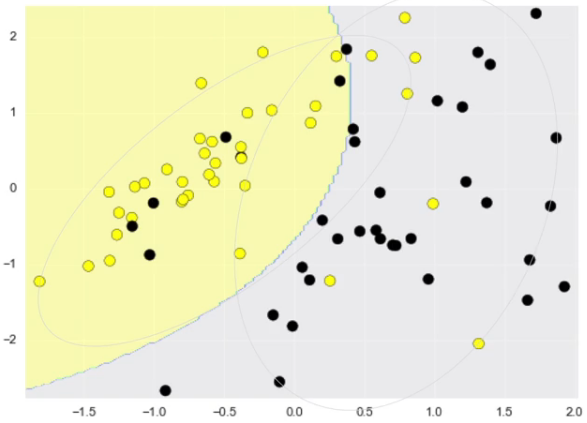
\includegraphics[width=\linewidth]{img/Gaussian-Naive-Bayes-Classifier-1.png} 
\end{center}


The line between the yellow and gray background areas represents the decision boundary. And we can see that this is indeed parabolic. 

To use the Gaussian Naive Bayes classifier in Python, 
we just instantiate an instance of the Gaussian NB class and call the fit method on the training data just as we would with any other classifier. 

\begin{verbatim}
from sklearn.naive_bayes import GaussianNB
\end{verbatim}

\textbf{Note:} the Naive Bayes models are among a few classifiers in scikit learn that support a method called \texttt{partial_fit},  which can be used instead of \texttt{fit} to train the classifier \emph{incrementally} in case you're working with a huge data set that doesn't fit into memory. 

For the \texttt{GaussianNB} class there are no special parameters to control the models complexity. 

Looking at one example in the notebook from our synthetic two class dataset, we can see that, in fact, the Gaussian Naive Bayes classifier achieves quite good performance on this simple classification example. When the classes are no longer as easily separable as with this second, more difficult binary example here. Like linear models, Naive Bayes does not perform as well. 

On a real world example, using the breast cancer data set, the Gaussian Naive Bayes Classifier also does quite well, being quite competitive with other methods, such as support vector classifiers. 

{\scriptsize
\begin{verbatim}
X_train, X_test, y_train, y_test = 
train_test_split(X_cancer, y_cancer, random_state = 0)

nbclf = GaussianNB().fit(X_train, y_train)
print('Breast cancer dataset')
print('Accuracy of GaussianNB classifier on training 
  set: {:.2f}'.format(nbclf.score(X_train, y_train)))
print('Accuracy of GaussianNB classifier on test set:
 {:.2f}'.format(nbclf.score(X_test, y_test)))

Breast cancer dataset
Accuracy of GaussianNB classifier on training set: 0.95
Accuracy of GaussianNB classifier on test set: 0.94
\end{verbatim}
}

Typically, Gaussian Naive Bayes is used for \emph{high-dimensional} data, when each data instance has hundreds, thousands or maybe even more features. Likewise the Bernoulli and Nultinomial flavors of Naive Bayes are used for text classification where there are very large number of distinct words is features and where the future vectors are sparse because any given document uses only a small fraction of the overall vocabulary. 

The Naive Bayes Classifiers are related mathematically to linear models, so many of the pros and cons of linear models also apply to Naive Bayes. 

On the \textbf{positive} side Naive Bayes classifiers are:
\begin{itemize}
\item easy to understand;
\item fast to train and use for prediction;
\item well suitable to high dimensional data including text and the applications involving very large data sets, where efficiency is critical and computational costs rule out other classification approaches;
\item often useful as a baseline comparison against more sophisticated methods.
\end{itemize}


On the \textbf{negative} side:
\begin{itemize}
\item assumption that features are conditionally independence are not realistic; for many real world datasets there's significant covariance among features;
\item other classifier types often have better generalization performance;
\item confidence estimates for predictions are not very accurate.
\end{itemize}

Other more sophisticated classification methods that can account for these dependencies are likely to outperform Naive Bayes. 

And on a side note, when getting confidence or probability estimates associated with predictions, Naive Bayes classifiers produce unreliable estimates, typically. 

Still, Naive Bayes Classifiers can perform very competitively on some tasks, and are also often very useful as baseline models against which more sophisticated models can be compared. 

\end{multicols}

\section{Random Forests}
\begin{multicols}{2}

A widely used and effective method in machine learning involves creating learning models known as \emph{ensembles}. An ensemble takes multiple individual learning models and combines them to produce an aggregate model that is more powerful than any of its individual learning models alone. 

Why are ensembles effective? Well, one reason is that if we have different learning models, although each of them might perform well individually, they'll tend to make different kinds of mistakes on the data set. And typically, this happens because each individual model might overfit to a different part of the data. By combining different individual models into an ensemble, we can average out their individual mistakes to reduce the risk of overfitting while maintaining strong prediction performance. 

Random forests are an example of the ensemble idea applied to decision trees. Random forests are widely used in practice and achieve very good results on a wide variety of problems. They can be used as classifiers via the sklearn \texttt{RandomForestClassifier} class or for regression using the \texttt{RandomForestRegressor} class both in the \texttt{sklearn.ensemble} module. 

As we saw earlier, one disadvantage of using a \emph{single} decision tree was that decision trees tend to be prone to overfitting the training data. 

As its name would suggest, a random forest creates lots of individual decision trees on a training set, often on the order of tens or hundreds of trees. The idea is that each of the individual trees in a random forest should do reasonably well at predicting the target values in the training set but should also be constructed to be different in some way from the other trees in the forest. 

Again, as the name would suggest this difference is accomplished by introducing random variation into the process of building each decision tree. 

\begin{center}
	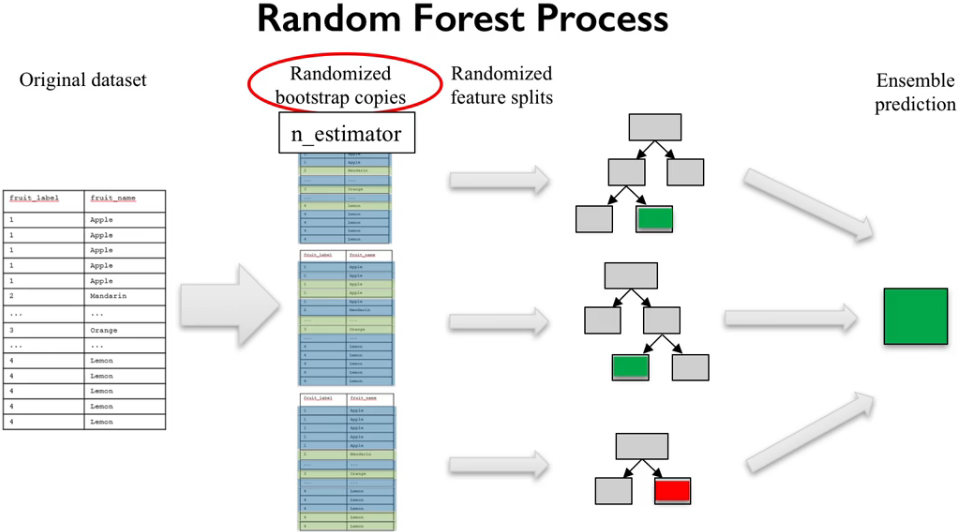
\includegraphics[width=\linewidth]{img/Random-Forest-Process.png} 
\end{center}


This random variation during tree building happens in two ways. First, the data used to build each tree is selected randomly and second, the features chosen in each split tests are also randomly selected. 

\subsection{Random Forests Model Creation}

To create a random forest model you first decide on how many trees to build. This is set using the \texttt{n_estimated} parameter for both RandomForestClassifier and RandomForestRegressor. Each tree were built from a different random sample of the data called the bootstrap sample. Bootstrap samples are commonly used in statistics and machine learning. If your training set has N instances or samples in total, a bootstrap sample of size N is created by just repeatedly picking one of the N dataset rows at random with replacement, that is, allowing for the possibility of picking the same row again at each selection. 

\begin{center}
	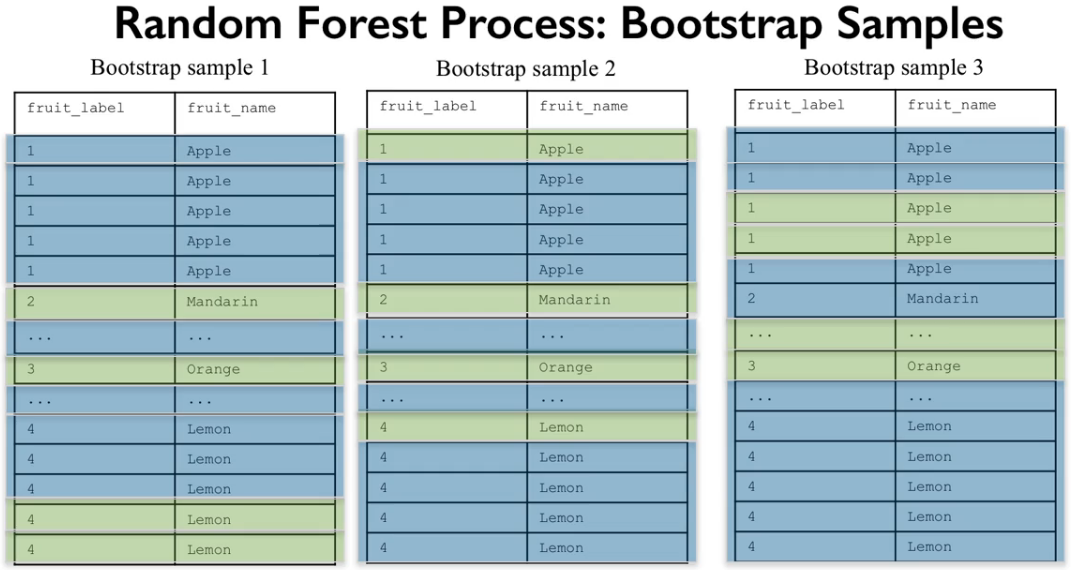
\includegraphics[width=\linewidth]{img/Bootstrap-Samples.png} 
\end{center}

You repeat this random selection process N times. The resulting bootstrap sample has N rows just like the original training set but with possibly some rows from the original dataset missing and others occurring multiple times just due to the nature of the random selection with replacement. 

When building a decision tree for a random forest, the process is almost the same as for a standard decision tree but with one important \emph{difference}. When picking the best split for a node, instead of finding the best split across all possible features, a \emph{random subset of features} is chosen and the best split is found within that smaller subset of features. The number of features in the subset that are randomly considered at each stage is controlled by the \texttt{max_features} parameter. 

This randomness in selecting the bootstrap sample to train an individual tree in a forest ensemble, combined with the fact that splitting a node in the tree is restricted to random subsets of the features of the split, virtually guarantees that all of the decision trees and the random forest will be different. 

The random forest model is quite sensitive to the \texttt{max_features} parameter. If \texttt{max_features = 1}, the random forest is limited to performing a split on the single feature that was selected randomly instead of being able to take the best split over several variables. This means the trees in the forest will likely be very different from each other and possibly with many levels in order to produce a good fit to the data. 

On the other hand if \texttt{max_features} is high, close to the total number of features that each instance has, the trees in the forest will tend to be similar and probably will require fewer levels to fit the data using the most informative features. 

\subsection{Prediction}

Once a random forest model is trained, it predicts the target value for new instances by first making a prediction for every tree in the random forest. 

\begin{center}
	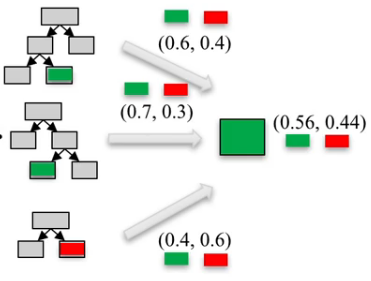
\includegraphics[width=\linewidth]{img/Random-Forest-Prediction.png} 
\end{center}

For \emph{regression} tasks the overall prediction is then typically the \textbf{mean} of the individual tree predictions. For \emph{classification} the overall prediction is based on a \textbf{weighted vote}. Each tree gives a probability for each possible target class label then the probabilities for each class are averaged across all the trees and the class with the highest probability is the final predicted class. 

\begin{center}
	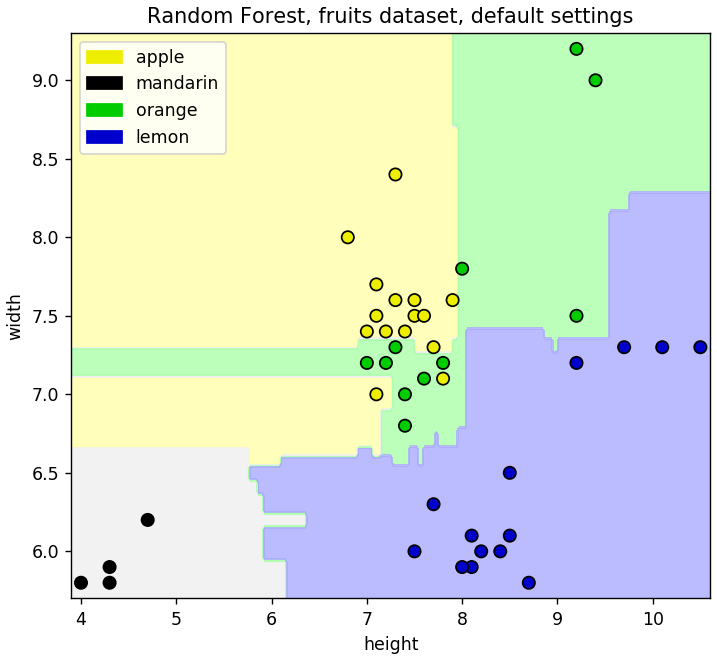
\includegraphics[width=\linewidth]{img/Random-Forest-Fruit-dataset.png} 
\end{center}

Here's an example of learning a random forest of the example fruit dataset using two features, height and width. Here we're showing the training data plotted in terms of two feature values with height on the x axis and width on the y axis. 

As usual, there are four categories of fruit to be predicted. Because the number of features is restricted to just two in this very simple example, the randomness in creating the tree ensemble is coming mostly from the bootstrap sampling of the training data. You can see that the decision boundaries overall have the \emph{box like shape} that we associate with decision trees but with some additional detail variation to accommodate specific local changes in the training data. 

Overall, you can get an impression of the increased complexity of this random forest model in capturing both the global and local patterns in the training data compared to the single decision tree model we saw earlier. 

\subsection{Implementation}

\subsubsection*{Fruit dataset}

Let's take a look at the notebook code that created and visualized this random forest on the fruit dataset.
{\scriptsize
\begin{verbatim}
from sklearn.ensemble import RandomForestClassifier
...
clf = RandomForestClassifier().fit(X, y)
clf = RandomForestClassifier(n_estimators = 10,
      random_state=0).fit(X_train, y_train)
...
Random Forest, Fruit dataset, default settings
Accuracy of RF classifier on training set: 1.00
Accuracy of RF classifier on test set: 0.80
\end{verbatim}
}

To use the \texttt{RandomForestClassifier} we import the random forest classifier class from the \texttt{sklearn.ensemble} library. 

For each pair of features we call the fit method on that subset of the training data X using the labels y. We then use the utility function plot class regions for classifier to visualize the training data and the random forest decision boundaries. 

Let's apply random forest to a larger dataset with more features. 

\subsubsection*{Breast Cancer dataset}

For comparison with other supervised learning methods, we use the breast cancer dataset. We create a new random forest classifier and since there are about 30 features, we'll set \texttt{max_features~=~8} to give a diverse set of trees that also fit the data reasonably well. 

{\scriptsize
\begin{verbatim}
Breast cancer dataset
Accuracy of RF classifier on training set: 1.00
Accuracy of RF classifier on test set: 0.99
\end{verbatim}
}

We can see that random forest with no feature scaling or extensive parameter tuning achieve very good test set performance on this dataset, in fact, it's as good or better than all the other supervised methods we've seen so far including current life support vector machines and neural networks that require more careful tuning. 

\textbf{Notice} that we did not have to perform scaling or other pre-processing as we did with a number of other supervised learning methods. This is one \emph{advantage} of using random forests. 

\subsection{Pros and Cons}

On the \textbf{positive} side of Random Forests:
\begin{itemize}
\item widely used, excellent prediction performance on many problems;
\item doesn't require careful normalization of features or extensive paramener tuning;
\item like decision trees, handles a mixture of feature types;
\item easily parallelized across multiple CPUs.
\end{itemize}

Even though building many different trees requires a corresponding increase in computation, building random forests is easily parallelized across multiple CPU's. 


On the \textbf{negative} side:
\begin{itemize}
\item the resulting modela are often difficult for humans to interpret~--- difficult to see the predictive structure of the features or to know why a particular prediction was made;
\item not a good choice for tasks that have very high dimensional sparse features like text classification.
\end{itemize}

\subsection{Key Parameters}

Here are some of the key parameters that you'll need for using random forests. 

\texttt{N_estimators} sets the number of trees to use. The default value for \texttt{n_estimators}~= 10 and increasing this number for larger data sets is almost certainly a good idea since ensembles that can average over more trees will reduce overfitting. 

Just bear in mind that increasing the number of trees in the model will also increase the computational cost of training. You'll use more time and more memory. So in practice you'll want to choose the parameters that make best use of the resources available on your system. 

The \texttt{max_features} parameter has a strong effect on performance. It has a large influence on how diverse the random trees in the forest are. Typically, the default setting of \texttt{max_features}, which for classification is the square root of the total number of features and for regression is the log base two of the total number of features, works quite well in practice although explicitly adjusting \texttt{max_features} may give you some additional performance gain with smaller values of max features tending to reduce overfitting. 

The \texttt{max_depth} parameter controls the depth of each tree in the ensemble. The default setting for this is none, in other words, the nodes in a tree will continue to be split until all leaves contain the same class or have fewer samples than the minimum sample split parameter value, which is two by default. 

The \texttt{n_jobs} parameter~--- how many cores to use in parallel to train the model. Generally, you can expect something close to a linear speed up. So, for example, if you have four cores, the training will be four times as fast as if you just used one. If you set end jobs to negative one it will use all the cores on your system and setting end jobs to a number that's more than the number of cores on your system won't have any additional effect. 

\end{multicols}

\section{Gradient Boosted Decision Trees}
\begin{multicols}{2}

Another tree based ensemble method that's gain wide use in real world application is gradient boosted decision trees~--- GBDT. 

Like random forest, gradient boosted trees used an ensemble of multiple tress to create more powerful prediction models for classification and regression. 

In this lecture, we'll provide a brief overview of gradient boosted decision trees, along with the discussion of their key parameters, the control model complexity. 

Unlike the random forest method that builds and combines a forest of randomly different trees in parallel, the key idea of gradient boosted decision trees is that they build a \emph{series} of trees. Where each tree is trained, so that it attempts to correct the mistakes of the previous tree in the series. 

\begin{center}
	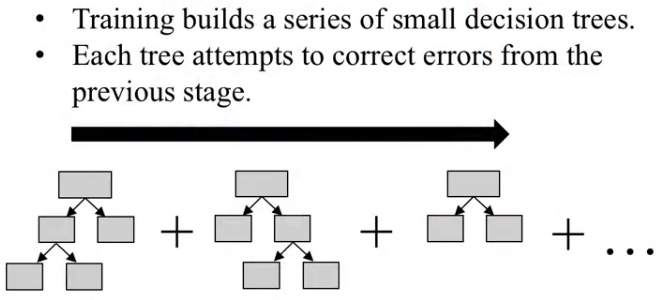
\includegraphics[width=\linewidth]{img/GBDT-1.png} 
\end{center}

Typically, gradient boosted tree ensembles use lots of shallow trees known in machine learning as \emph{weak learners}. Built in a \emph{non-random} way, to create a model that makes fewer and fewer mistakes as more trees are added.  

Once the model is built, making predictions with a gradient boosted tree models is fast and doesn't use a lot of memory. 

\begin{center}
	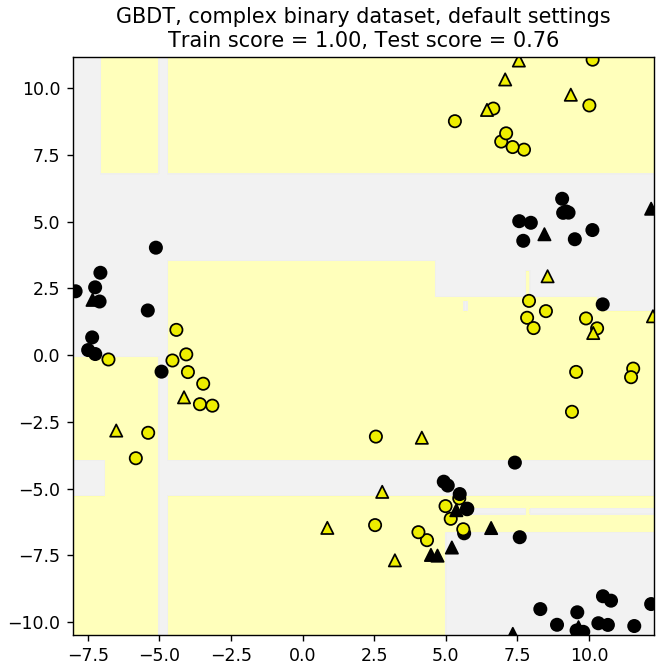
\includegraphics[width=\linewidth]{img/GBDT-3.png} 
\end{center}


Like random forests, the \texttt{number of estimators} in the gradient boosted tree ensemble is an important parameter in controlling model complexity. 

A new parameter that does not occur with random forest is something called the \texttt{learning_rate}. The learning rate controls how the gradient boost the tree algorithms builds a series of collective trees. When the learning rate is \emph{high}, each successive tree puts strong emphases on correcting the mistakes of its predecessor, and thus may result in a more complex individual tree, and those overall are more complex model. With \emph{smaller} settings of the learning rate, there's less emphasis on thoroughly correcting the errors of the previous step, which tends to lead to simpler trees at each step. 

{\scriptsize
\begin{verbatim}
from sklearn.ensemble import GradientBoostingClassifier
from sklearn.model_selection import train_test_split

X_train, X_test, y_train, y_test = 
    train_test_split(X_D2, y_D2, random_state = 0)

clf = GradientBoostingClassifier().fit(X_train, y_train)
...
GBDT, Fruit dataset, default settings
Accuracy of GBDT classifier on training set: 1.00
Accuracy of GBDT classifier on test set: 0.80
\end{verbatim}
}


\begin{center}
	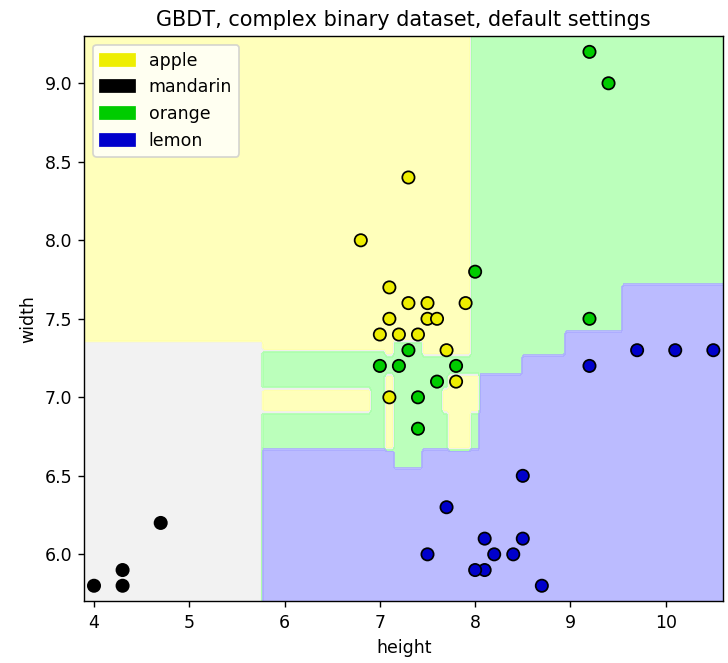
\includegraphics[width=\linewidth]{img/GBDT-4.png} 
\end{center}

Here's an example showing how to use gradient boosted trees in scikit-learn on our sample fruit classification test, plotting the decision regions that result. The code is more or less the same as what we used for random forests. 

But from the sklearn.ensemble module, we import the \texttt{GradientBoostingClassifier} class. We then create the \texttt{GradientBoostingClassifier} object, and fit it to the training data in the usual way. By default, the \texttt{learning rate} parameter is set to \textbf{0.1}, the \texttt{n_estimators} parameter giving the number of trees to use is set to \textbf{100}, and the \textbf{max_depth} is set to \textbf{3}. As with random forests, you can see the decision boundaries have that box-like shape that's characteristic of decision trees or ensembles of trees. 

Now let's apply gradient boosted decision trees to the breast cancer dataset. This code trains two different gradient boosted classifiers. The first one uses the default settings. 

{\scriptsize
\begin{verbatim}
Breast cancer dataset (learning_rate=0.1, max_depth=3)
Accuracy of GBDT classifier on training set: 1.00
Accuracy of GBDT classifier on test set: 0.96

Breast cancer dataset (learning_rate=0.01, max_depth=2)
Accuracy of GBDT classifier on training set: 0.97
Accuracy of GBDT classifier on test set: 0.97
\end{verbatim}
}

We can see that the first result has perfect accuracy on the training set, which indicates the model is likely overfitting. 

Two ways to learn a less complex gradient boosted tree model are, to reduce the \texttt{learning_rate}, so that each tree doesn't try as hard to learn a more complex model, that fixes the mistakes of its predecessor. And to reduce the \texttt{max_depth} parameter for the individual trees in the ensemble. 

The second classifier example makes these changes in the parameters. And you can see, that the training set accuracy does decrease, while the test set accuracy increases slightly. 

\subsection{Pros and Cons}

Gradient boosted decision trees are among the best off-the-shelf supervised learning methods available. Achieving excellent accuracy with only modest memory and runtime requirements to perform prediction, once the model has been trained. 

Some major commercial applications of machine learning have been based on gradient boosted decision trees. 

Like other decision tree based learning methods, you don't need to apply feature scaling for the algorithm to do well. And the futures can be a mix of binary, categorical and continuous types. 

Boosted decision trees do have several downsides. So like random forests, ensembles of trees are very difficult for people to interpret, compared to individual decision trees. However, this often may not matter for many applications where prediction accuracy is the most important goal. 

Gradient boosted methods can require careful tuning of the learning rate and other parameters. And the training process can require a lot of computation. 

And like the other tree based methods we saw, using gradient boosted methods for text classification or other scenarios. Where the featured space has thousands of features with sparse values, is usually not a good choice for accuracy and computational cost reasons. 

\subsection{Key Parameters}

The key parameters controlling model complexity for gradient boosted tree models are, \texttt{n_estimators} which sets the number of small decisions trees the week learns to use in the ensemble, and the \texttt{learning_rate}. 

Typically, these two parameters are tuned together. Since making the learning rates smaller, will require more trees to maintain model complexity. 

Unlike random forest, increasing an \texttt{n_estimators} can lead to overfeeding. So typically, the \texttt{n_estimators} setting is chosen to best exploit the speed and memory capabilities of the system during the training. And other parameters like the \texttt{learning_rate} are then adjusted, given that fixed an n_estimators setting. 

The \texttt{max_depth} parameter can also have an effect of model complexity, but controlling the depth, and has a complexity of the individual trees. The gradient boosting method assumes, that each trees is a weak learner, and so the \texttt{max_depth} parameter is usually quite small, on the order of three to five, for most applications. 

\end{multicols}

\section{Neural-Networks}
\begin{multicols}{2}

In this part of the course, you'll get an introduction to the basics of neural networks. Which are a broad family of algorithms that have formed the basis for the recent resurgence in the computational field called deep learning. Early work on neural networks actually began in the 1950s and 60s. And just recently, has experienced a resurgence of interest, as deep learning has achieved impressive state-of-the-art results. On specific tasks that range from object classification in images, to fast accurate machine translation, to gameplay. 

The topic of neural networks requires its own course. And indeed, if you're interested in more depth, you can check out the excellent course on Coursera. Called Neural Networks for Machine Learning, by a pioneer in this area, Professor Jeff Hinton. 

Here, we'll provide an introduction to the basic concepts and algorithms that are foundation of neural networks. And of the much more sophisticated deep learning methods in use today. You'll learn about some basic models called \emph{multi-layer perceptrons}, supported by \texttt{scikit-learn}, that can be used for classification and regression. 

Let's start by briefly reviewing simpler methods we have already seen for regression and classification. 

\begin{center}
	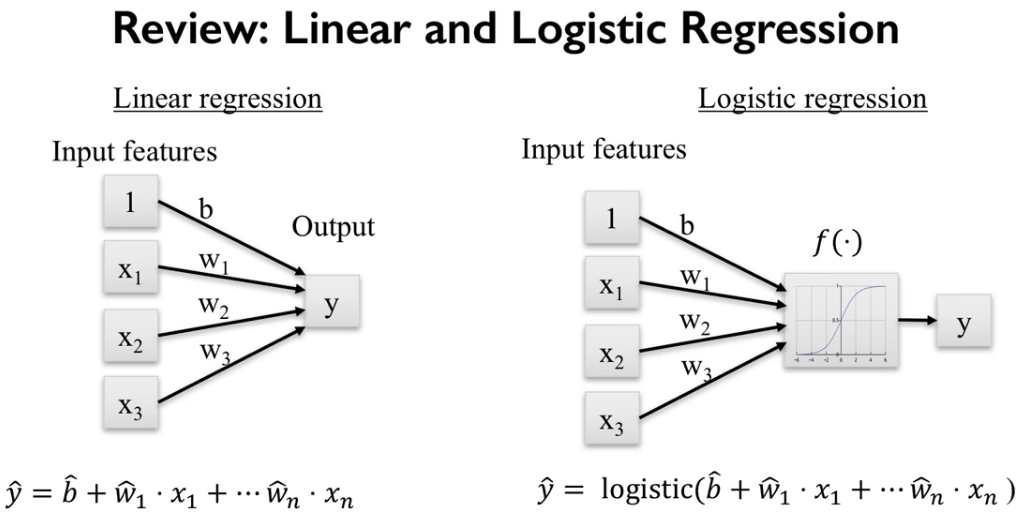
\includegraphics[width=\linewidth]{img/Linear-Regression-Logistic-Regression.png} 
\end{center} 

Linear regression predicts a continuous output, $\hat{y}$, shown as the box on the right. As a function as the sum of the input variables $x_i$, shown in the boxes on the left. 

Each weighted by a corresponding coefficient, $\hat{w}_i$, plus an intercept or bias term, $\hat{b}$. We saw how various methods like ordinary least squares, ridge regression or lasso regression. Could be used to estimate these model coefficients, $\hat{w}_i$, and $\hat{b}$, shown above the arrows in the diagram, from training data. 

Logistic regression takes this one step further, by running the output of the linear function of the input variables, $x_i$. Through an additional nonlinear function, the logistic function. Represented by the new box in the middle of the diagram, to produce the output, $y$. 

Which, because of the logistic function, is now constrained to lie between 0 and 1. 

We use \emph{logistical regression} for \emph{binary classification}. Since we can interpret $y$ as the \emph{probability} that a given input data instance belongs to the positive class, in a two-class binary classification scenario. 

Here's an example of a simple neural network for regression, called a multi-layer perceptron (MLP). These are also known as \emph{feed-forward neural networks}.

\begin{center}
	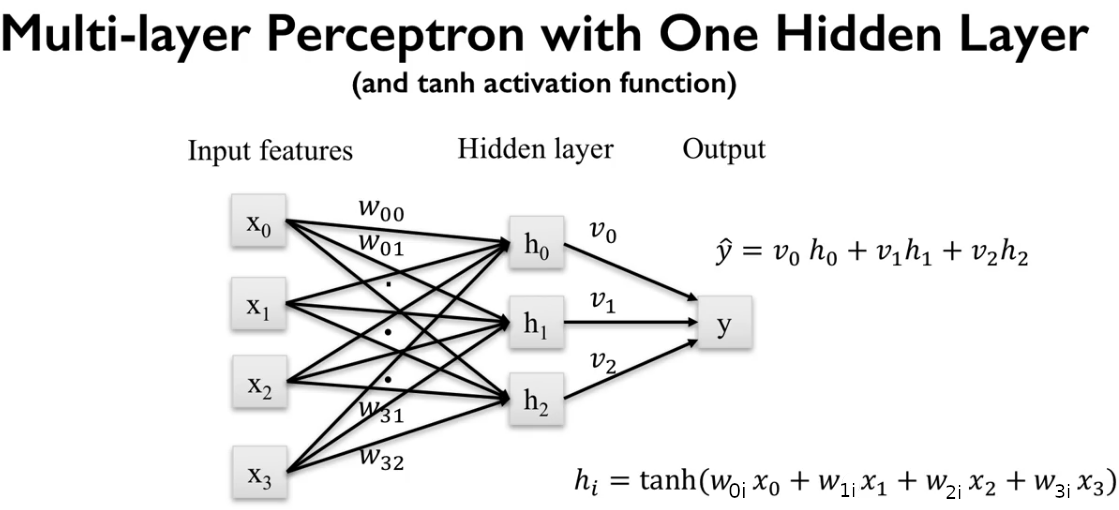
\includegraphics[width=\linewidth]{img/Multi-layer-Perseptron.png} 
\end{center}

MLPs take this idea of computing weighted sums of the input features, like we saw in logistic regression. But it takes it a step beyond logistic regression, by adding an additional processing step called a \emph{hidden layer}. Represented by this additional set of boxes, $h_0$, $h_1$ and $h_2$ in the diagram. These boxes, within the hidden layer, are called \emph{hidden units}. And each hidden unit in the hidden layer computes a \emph{nonlinear} function of the weighted sums of the input features. Resulting in \emph{intermediate} output values, $v_0, v_1, v_2$. Then the MLP computes a weighted sum of these hidden unit outputs, to form the final output value, $\hat{y}$. 

This nonlinear function that the hidden unit applies. is called the \emph{activation function}. In this example, your activation function is the hyperbolic tangent function, which is related to the logistic function. You can see that the result of adding this additional hidden layer processing step to the prediction model, is a formula for $\hat{y}$. That is already more involved than the one for logistic regression. Now predicting $\hat{y}$ involves computing a different initial weighted sum of the input feature values for each hidden unit. Which applies a nonlinear activation function. And then all of these nonlinear outputs are combined, using another weighted sum, to produce $\hat{y}$. 

In particular, there's one weight between each input and each hidden unit. 
And one weight between each hidden unit and the output variable. 

In fact, this addition and combination of non-linear activation functions allows multi-layer perceptrons to learn more complex functions than is possible with a simple linear or logistic function. This additional expressive power enables neural networks to perform more accurate prediction when the relationship between the input and output is itself complex. 

Of course, this complexity also means that there are a lot more weights, model coefficients, to estimate in the training phase. Which means that both \emph{more training data and more computation} are typically needed to learn in a neural network, compared to a linear model. 

As an aside, there are a number of choices for the activation function in a neural network, that gets applied in hidden units. 

\begin{center}
	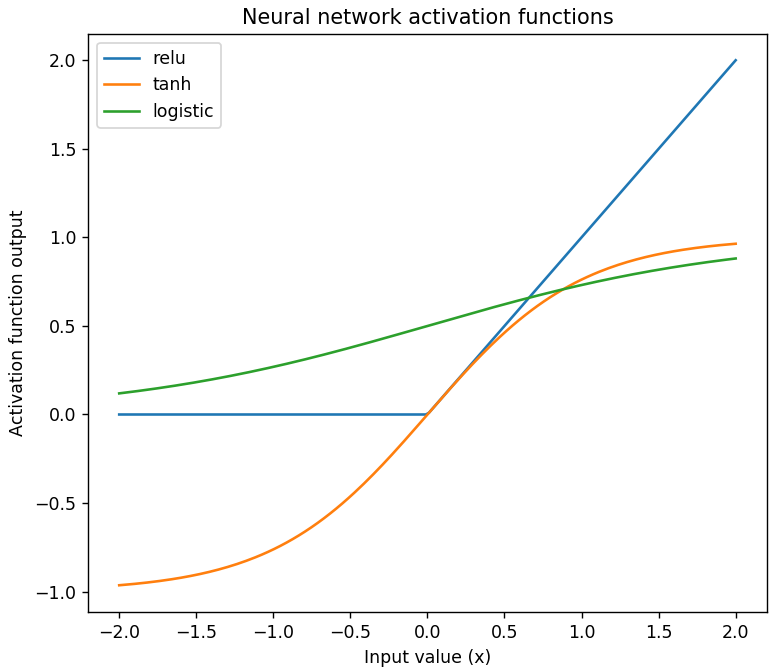
\includegraphics[width=\linewidth]{img/Neural-Network-Activation-Functions.png} 
\end{center}

Here, the plot shows the input value coming into the activation function, from the previous layer's inputs on the x-axis. And the y-axis shows the resulting output value for the function. 

The three main activation functions we'll compare later in this lecture are:
\begin{itemize}
\item the hyperbolic tangent
\item the rectified linear unit function (relu)
\item the logistic function
\end{itemize}

The relu activation function is the default activation function for neural networks in scikit-learn. It maps any negative input values to zero. 

The hyperbolic tangent function, or tanh function maps large positive input values to outputs very close to one. And large negative input values, to outputs very close to negative one. 

These differences in the activation function can have some effect on the shape of regression prediction plots or classification decision boundaries that neural networks learn. 

In general, we'll be using either the hyperbolic tangent or the relu function as our default activation function. Since these perform well for most applications. 

\subsection{Implementation}

Let's take a look at how we use neural networks in scikit-learn for classification. Using the more complex synthetic binary classification data set. 

To use a neural network classifier, you import the MLPClassifier class from the \texttt{sklearn.neural} network module. 

{\scriptsize
\begin{verbatim}
from sklearn.neural_network import MLPClassifier
\end{verbatim}
}

This code example shows the classifier being fit to the training data, using a single hidden layer. With three different numbers of hidden units in the layer, 1 unit, 10 units and 100 units. As with all other classification types we've seen, you can create the classifier objects with the appropriate parameters. And call the fit method on the training data. 

Here, the main parameter for a neural network classifier is this parameter, \texttt{hidden_layer_sizes}. 

This parameter is a list, with one element for each hidden layer, that gives the number of hidden units to use for that layer. So here we're passing a list with a single element. Meaning we want one hidden layer, using the number in the variable called units. 

By default, if you don't specify the \texttt{hidden_layer_sizes} parameter, scikit-learn will create a single hidden layer with 100 hidden units. While a setting of 10 may work well for simple data sets, like the one we use as examples here. For really complex data sets, the number of hidden units could be in the thousands. It's also possible, as we'll see shortly, to create an MLP with more than one hidden layer. By passing a \texttt{hidden_layer_sizes} parameter with multiple entries. 

I want to also note the use of this extra parameter, called \texttt{solver}. Which specifies the algorithm to use for learning the weights of the network. 

Here, we're using the lbfgs algorithm. We'll discuss the \texttt{solver} parameter setting further, at the end of this lecture. 

Also note that we're passing in a \texttt{random_state} parameter, when creating the MLPClassifier object. Like we did for the train-test split function. And we happened to set this \texttt{random_state} parameter to a fixed value of 0. 

This is because for neural networks, their weights are initialized randomly, which can affect the model that is learned. 

Because of this, even without changing the key parameters on the same data set. The same neural network algorithm might learn two different models. Depending on the value of the internal random seed that is chosen. So by always setting the same value for the random seed used to initialize the weights. We can assure the results will always be the same, for everyone using these examples. 

This graphic plots the results of running this code. To show how the number of hidden units in a single layer in the neural network affects the model complexity for classification. 

\begin{center}
	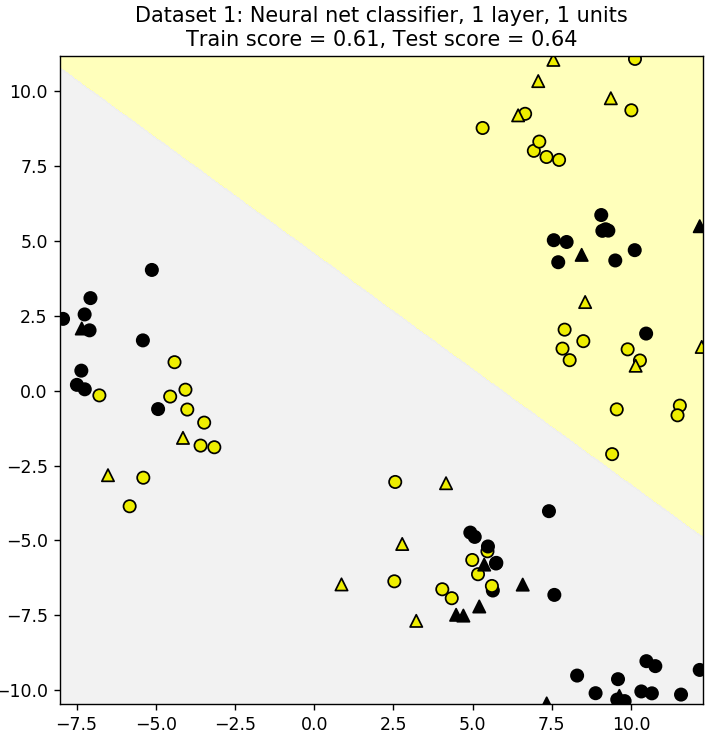
\includegraphics[width=\linewidth]{img/Neural-net-classifier-1layer-1unit.png} 
\end{center}

With 1 hidden unit, the model is mathematically equivalent to logistic regression. We see the classifier returns the familiar simple linear decision boundary between the two classes. The training set score's low, and the test score is not much better, so this network model is under-fitting. 

\begin{center}
	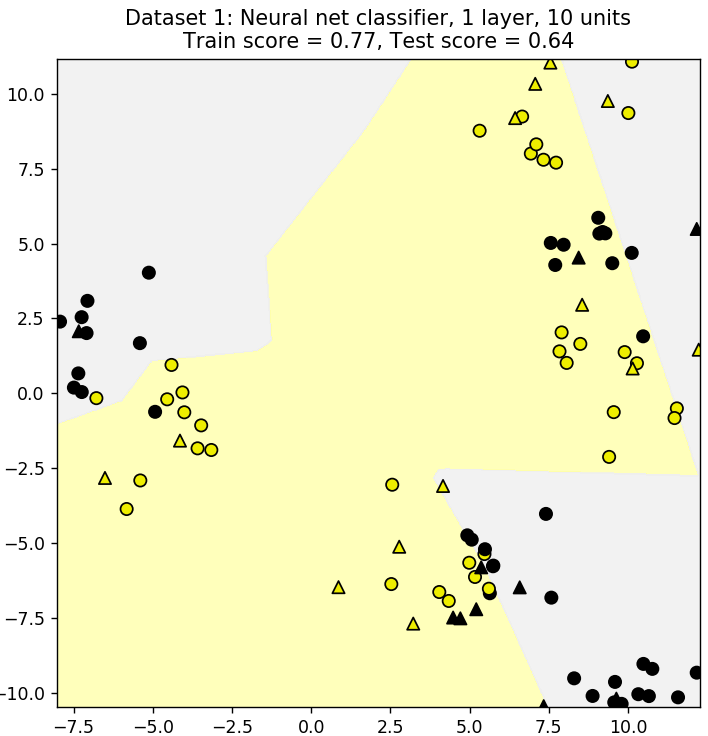
\includegraphics[width=\linewidth]{img/Neural-net-classifier-1layer-10units.png} 
\end{center}

With 10 hidden units, we can see that the MLPClassifier is able to learn a more complete decision boundary. That captures more of the nonlinear, cluster-oriented structure in the data, though the test set accuracy is still low. 

\begin{center}
	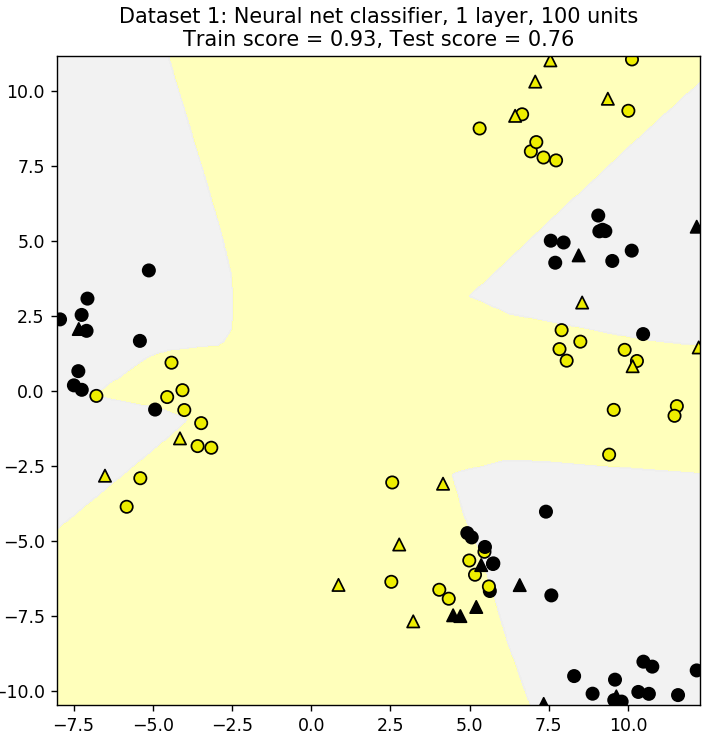
\includegraphics[width=\linewidth]{img/Neural-net-classifier-1layer-100units.png} 
\end{center}

With 100 hidden units, the decision boundary is even more detailed. And achieves much better accuracy, on both the training and the test sets. 

\subsection{Multi-layer Perceptron}

Here's a graphical depiction of a multi-layer perceptron with two hidden layers. 

\begin{center}
	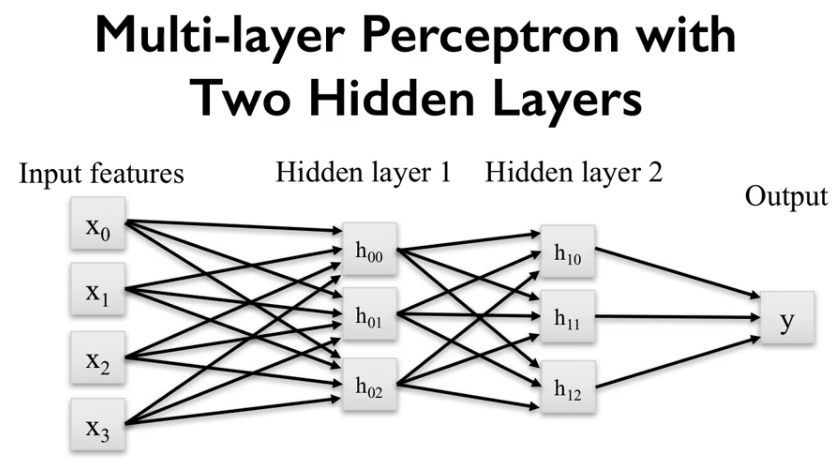
\includegraphics[width=\linewidth]{img/Multi-layer-Perseptron-2Hidden-layers.png} 
\end{center}

Adding the second hidden layer further increases the complexity of functions that the neural network can learn, from more complex data sets. 

Taking this complexity further, large architectures of neural networks, with many stages of computation, are why \emph{deep learning} methods are called deep. 

Here is an example in the notebook, showing how we create a two-layer MLP, with 10 hidden units in each layer. 

{\scriptsize
\begin{verbatim}
nnclf = MLPClassifier(hidden_layer_sizes = [10, 10], 
    solver='lbfgs').fit(X_train, y_train)
\end{verbatim}
}

We just set the \texttt{hidden_layer_sizes} parameter, when creating the MLPClassifier, to a two-element list, indicating ten units, in each of the two hidden layers. 

You can see the result of of adding the second hidden layer, on the classification problem we saw earlier. 

\begin{center}
	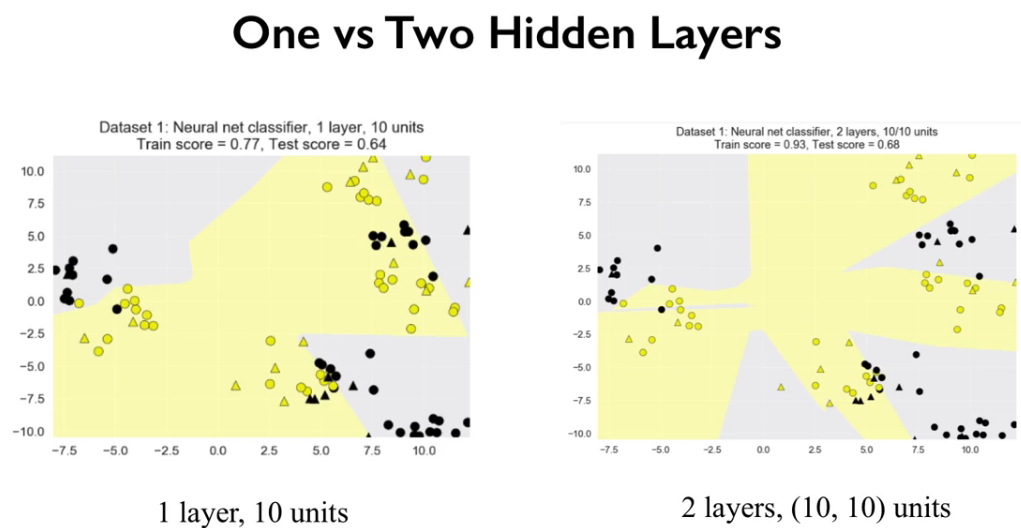
\includegraphics[width=\linewidth]{img/One-vs-Two-Hidden-Layers.png} 
\end{center}

On the left is the original MLP, with one hidden layer of ten units. And on the right is the same data set, using a new MLP with two hidden layers of ten units each. You can see the MLP with two hidden layers learned a more complex decision boundary. And achieved, in this case, a much better fit on the training data, and slightly better accuracy on the test data. 

Once we start adding more hidden layers, with lots of hidden units. You can see that the number of weights, or model coefficients, to estimate for a neural network can increase rapidly. So that more complex neural networks could have many thousands of weights to estimate. 

\subsection{Regularization}

We can control this model complexity, just as we did with ridge and lasso regression, by adding an L2 regularization penalty on the weights. Remember that L2 regularization penalizes models that have a large sum of squares of all the weight values with the effect being that the neural network prefers models with more weights shrunk close to zero. 

The regularization parameter for MLPs is called \texttt{alpha}, like with the linear regression models. And in scikit-learn, it's set to a small value by default, like 0.0001, that gives a little bit of regularization. 

{\scriptsize
\begin{verbatim}
for this_alpha, axis in 
    zip([0.01, 0.1, 1.0, 5.0], subaxes):
    nnclf = MLPClassifier(solver='lbfgs', 
               activation = 'tanh',
               alpha = this_alpha,
               hidden_layer_sizes = [100, 100],
               random_state = 0).fit(X_train, y_train)
\end{verbatim}
}


This code example shows the effects of changing alpha for a larger MLP, with 2 hidden layers of 100 nodes each. From a small value of 0.01, to a larger value of 5.0. For variety here, we're also setting the activation function to use the hyperbolic tangent function. 

Here's the graphical output of this notebook code. You can see the effect of increasing regularization with increasing alpha. 

\begin{center}
	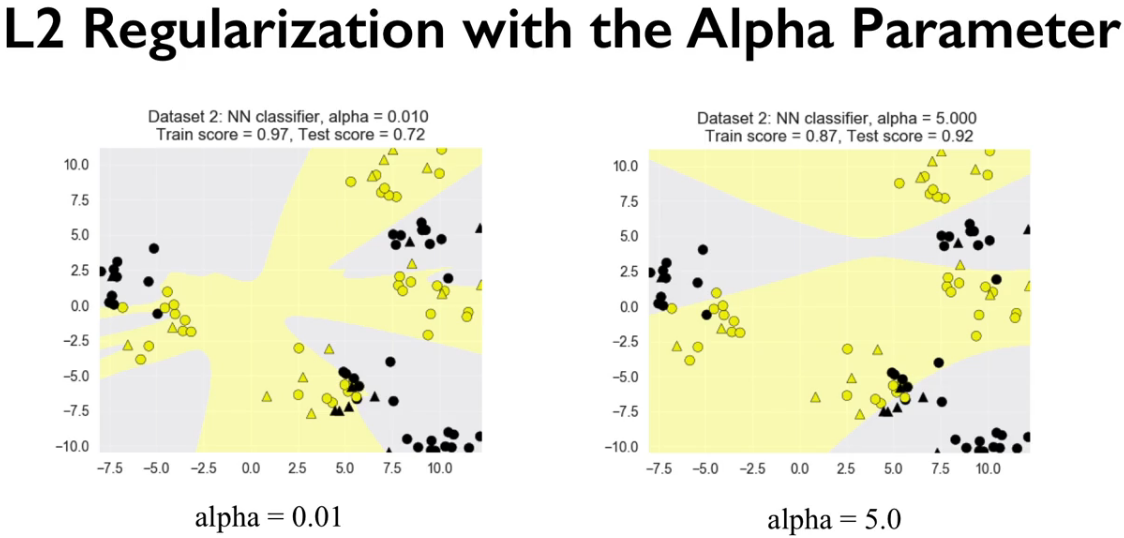
\includegraphics[width=\linewidth]{img/Neural-Network-L2-Regularization.png} 
\end{center}

In the left plot, when alpha is small, the decision boundaries are much more complex and variable. And the classifier's over-fitting, as we can see from the very high training set score, and low test score. On the other hand, the right plot uses the largest value of alpha here, alpha 5.0. And that setting results in much smoother decision boundaries, while still capturing the global structure of the data. And this increased simplicity allows it to generalize much better, and not over-fit to the training set. And this is evident from the much higher test score, in this case. 

\subsection{Features Normalization}

As with other supervised learning models, like regularized regression and support vector machines, it can be \textbf{critical}, when using neural networks, to \emph{properly normalize the input features}. 

Let's apply the multi-layer perceptron to the breast cancer data set. And notice that we first apply the \texttt{MinMaxScaler}, to pre-process the input features. 

Here we'll combine a more complex network, using 2 hidden layers with 100 units each. With a higher regularization setting of alpha at 5.0, and using the lgbfs solver again. 

{\tiny
\begin{verbatim}
from sklearn.neural_network import MLPClassifier
from sklearn.preprocessing import MinMaxScaler

scaler = MinMaxScaler()

X_train, X_test, y_train, y_test = train_test_split(X_cancer, y_cancer,
                                                    random_state = 0)
X_train_scaled = scaler.fit_transform(X_train)
X_test_scaled = scaler.transform(X_test)

clf = MLPClassifier(hidden_layer_sizes = [100, 100], alpha = 5.0,
      random_state = 0, solver='lbfgs').fit(X_train_scaled, y_train)

print('Breast cancer dataset')
print('Accuracy of NN classifier on training set: {:.2f}'
     .format(clf.score(X_train_scaled, y_train)))
print('Accuracy of NN classifier on test set: {:.2f}'
     .format(clf.score(X_test_scaled, y_test)))
     
Breast cancer dataset
Accuracy of NN classifier on training set: 0.98
Accuracy of NN classifier on test set: 0.97 
\end{verbatim}
}

You can see, that with this multi-layer perceptron, both the training and test set accuracy are among the highest we have obtained on this data set. 

\subsection{Regression}

Like many of the other supervised learning methods we've seen, you can also use multi-layer perceptrons for regression, as well as classification. 

We're including MLP regression here, as an example, for two reasons. First, because MLP regression may be useful for some regression problems on its own. But more generally, because some deep learning problems are regression problems. 

And so, as with classification, using multi-layer perceptrons is a good starting point to learn about the more complex architectures used for regression in deep learning. 

{\tiny
\begin{verbatim}
from sklearn.neural_network import MLPRegressor

fig, subaxes = plt.subplots(2, 3, figsize=(11,8), dpi=70)

X_predict_input = np.linspace(-3, 3, 50).reshape(-1,1)

X_train, X_test, y_train, y_test = 
    train_test_split(X_R1[0::5], y_R1[0::5], random_state = 0)

for thisaxisrow, thisactivation in zip(subaxes, ['tanh', 'relu']):
    for thisalpha, thisaxis in zip([0.0001, 1.0, 100], thisaxisrow):
        mlpreg = MLPRegressor(hidden_layer_sizes = [100,100],
                             activation = thisactivation,
                             alpha = thisalpha,
                             solver = 'lbfgs').fit(X_train, y_train)
        y_predict_output = mlpreg.predict(X_predict_input)
        thisaxis.set_xlim([-2.5, 0.75])
        thisaxis.plot(X_predict_input, y_predict_output,
                     '^', markersize = 10)
        thisaxis.plot(X_train, y_train, 'o')
        thisaxis.set_xlabel('Input feature')
        thisaxis.set_ylabel('Target value')
        thisaxis.set_title('MLP regression\nalpha={}, activation={})'
                          .format(thisalpha, thisactivation))
        plt.tight_layout()
\end{verbatim}
}        
        
You use the multi-layer perceptron regressor by importing the MLPRegressor class from the sklearn.neural_network module, and then creating the MLPRegressor object. When creating the object here, we're setting the number of hidden layers and units within each hidden layer. Using the same \texttt{hidden_layer_sizes} parameter that we used for classification. 

This example uses two hidden layers, with 100 hidden nodes each. This notebook code has a loop that cycles through different settings of the \texttt{activation_function} parameter, and the \texttt{alpha} parameter for L2 regularization. 

Here we've included regression results that use, in the top row, the hyperbolic tangent activation function. And in the bottom row, the relu activation function. 


You can see the \emph{smoothness} of the activation function somewhat influences the smoothness of the corresponding regression results. 

Along the columns, the plots also show the effect of using different alpha settings, to increase the amount of L2 regularization from left to right. 

Again, as with classification, the effect of increasing the amount of L2 regularization, by increasing alpha. Is to constrain the regression to use simpler and simpler models, with fewer and fewer large weights. 

You can see this effect for both activation functions, in the top and bottom rows. The regression line on the left has higher variance than the much smoother, regularized model on the right. 

\end{multicols}
\begin{center}
	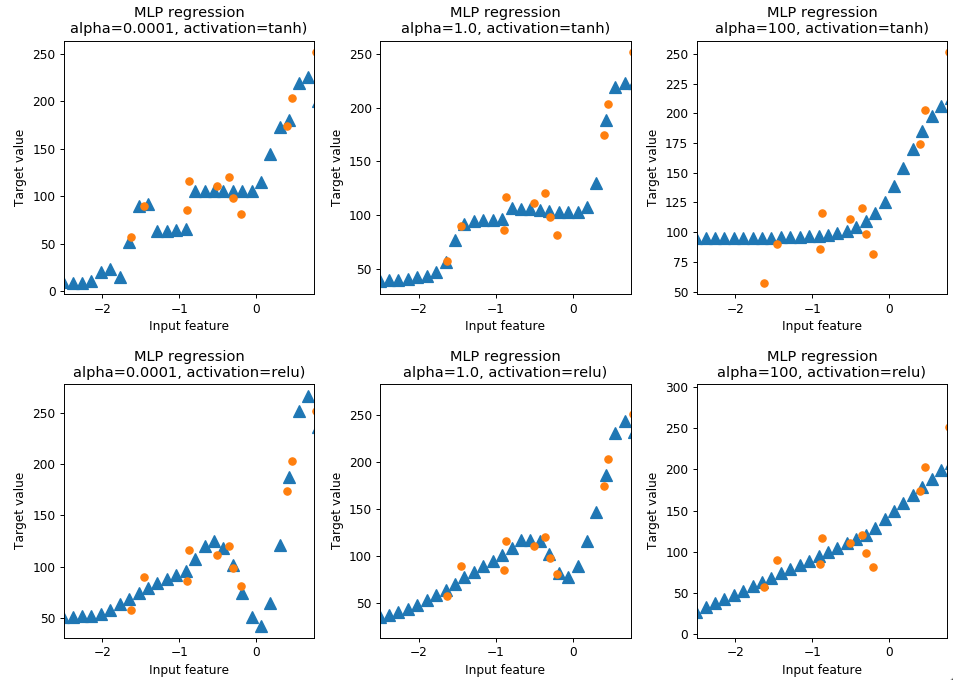
\includegraphics[width=\linewidth]{img/Neural-Networks-Regression.png} 
\end{center}
\begin{multicols}{2}

\subsection{Pros and Cons}

On the positive side, beyond these simple examples we've shown here. Neural networks form the basis of advanced learning architectures. That capture complex features, and give state-of-the-art performance on an increasingly wide variety of difficult learning tasks. 

From world-championship play for the game of Go, to detailed and robust recognition of objects and images. 

However, with this increased power, come increased costs. This larger and more complex models typically \emph{require significant volumes of data, computation, and training time} to learn. 

In addition, \emph{careful pre-processing of the input data} is needed, to help ensure fast, stable, meaningful solutions to finding the optimal set of weights. 

In general, neural networks are a good choice, when the features are of \emph{similar} types. For example, all derived from the pixels of an image. And less of a good choice, when the features are of very different types. 

\subsection{Key Parameters}

Finally, let's review the key parameters for the multi-layer perceptron in scikit-learn, that can be used to control model complexity. 

The main way to control model complexity for the MLP, is to control the hidden unit size and structure. Using the \texttt{hidden_layers_sizes} parameter that controls the number of hidden layers~--- number of elements in list, and the number of units within each layer. Default: \texttt{hidden_layers_sizes = 100}.

\texttt{Alpha} controls the amount of regularization that helps constrain the complexity of the model, by constraining the magnitude of model weights. Default: \texttt{alpha = 0.0001}

Finally, you can experiment with at least three different choices for the nonlinear activation function, by using the \texttt{activation} parameter: \texttt{relu}~--- default, \texttt{logistic} and \texttt{tahn}. 

Earlier, we saw the \texttt{solver} parameter, for specifying the algorithm that learns the network weights. 

\texttt{Solver} is the algorithm that actually does the numerical work of finding the optimal weights. And one intuitive way of visualizing this  process is that all of the solver algorithms have to do a kind of hill-climbing in a very bumpy landscape, with lots of local minima. 

Where each local minimum corresponds to a locally optimal set of weights. That is, a choice of weight setting that's better than any nearby choices of weights. So across this whole landscape of very bumpy local minima. Some will have higher validation scores on the test data, and some will have lower. So depending on the initial random initialization of the weights. And the nature of the trajectory in the search path that a solver takes through this bumpy landscape. The solver can end up at different local minima, which can have different validation scores. 

The default solver, \texttt{adam}, tends to be both efficient and effective on large data sets, with thousands of training examples. 

For \emph{small} data sets, like many of the ones we use in these examples, the \texttt{lbfgs} solver tends to be faster, and find more effective weights.
\end{multicols}

\section{Deep Learning}
\begin{multicols}{2}

As we discussed in the first week of the course, one of the key challenges in machine learning is finding the right features to use as input to a learning model for a particular problem. This is called f\emph{eature engineering} and can be part art, and part science. It can also be the single most factor in doing well on a learning task. Sometimes, in fact, more often more important than the choice of the model itself. 
We'll discuss this further in the last week of the course. 

Because of the difficulty of feature engineering, there's been a lot of research on what's called \emph{feature learning} or \emph{feature extraction} algorithms that can find good features \emph{automatically}. This brings us to deep learning. 

At a high-level, one of the advantages of deep learning is that it includes a sophisticated automatic featured learning phase as part of its supervised training. Moreover, deep learning is called deep because this feature extraction typically doesn't use just one feature learning step, but a \emph{hierarchy} of multiple feature learning layers. Each feeding into the next.

Here's one simplified example of what a deep learning architecture might look like in practice for an image recognition task. In this case, digit recognition.

\begin{center}
	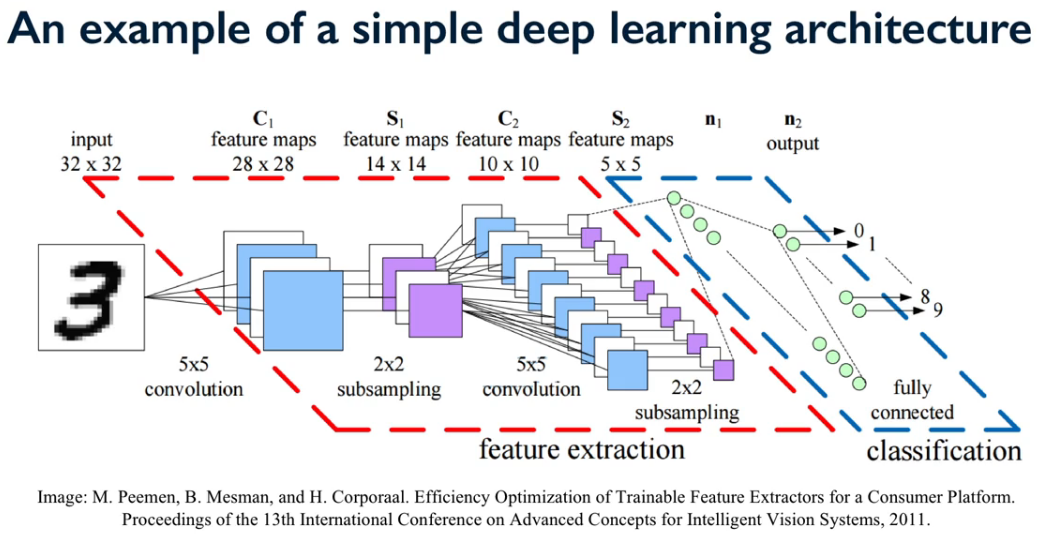
\includegraphics[width=\linewidth]{img/Deep-Learning-Architecture.png} 
\end{center} 

Recognizing a handwritten digit from zero to nine, for example. You can see the \emph{automatic feature extraction step} made up of hierarchy of feature layers. Each of which is based on a network that does \emph{convolution} which can be thought of as a filter for a specific pattern followed by a \emph{subsampling} step, also known as \emph{pooling} that can detect a translated or rotated version of that feature anywhere in the image. So that features are detected properly for the final classification step, which is implemented as a fully connected network. The subsampling step also has the effect of \emph{reducing the computational complexity} of the network. Depending on the properties of the object we want to predict, for example. If we care only about the presence of the object in the image compared to let's say, specific location, the subsampling part of the architecture may or may not be included and this is only one example of a deep learning architecture. The size, structure and other properties may look very different. Depending on the specific learning problem. 

This image from a paper by Honglak Lee and colleagues at the University of Michigan shows an illustration of multilayer feature learning for face recognition. 

Here there are three groups from left to right corresponding to first, second and third stages of feature learning. The matrix at each stage shows a set of image features with one feature per square. Each feature can be thought of as a detector or filter, that lights up when that pattern is present in the underlying image. The first layer of their deep learning architecture extracts the most primitive low-level features, such as edges and different kinds of blobs. 

The second layer creates new features from combinations of those first layer features. For faces, this might correspond to key elements that capture shapes of higher level features like noses or eyes. 

The third layer in turn, creates new features from combinations of the second layer of features. Forming still higher level features that capture typical face types and facial expressions. Finally, all of these features are used as input to the final supervised learning step, namely the face classifier. Here are the feature layers that result from training on different types of objects, cars, elephants, chairs and a mixture of objects. 

These kinds of complex features can't be learned from a small number of layers. Advances in both algorithms and computing power allow current deep learning systems to train architectures that could have dozens of layers of nonlinear, hierarchical features. It turns out that the human brain does something quite related to this when processing visual information. There are specific neurocircuits that first do low-level feature extraction, such as edge detection and finding the frequency of repeated patterns which are then used to compute more sophisticated features to help estimate things like simple shapes and their orientation or whether a shape is in the foreground or background. Followed by further layers of higher level visual processing that support more complex tasks, such as face recognition and interpreting the motion of multiple moving objects.

\subsection{Pros and Cons}

On the \textbf{positive} side, deep learning systems have achieved impressive gains and have achieved state-of-the-art \emph{performance} on many difficult tasks. 

Deep learning's automatic feature extraction mechanisms also \emph{reduce the need for human guesswork} in finding good features. 

Finally, with current software, deep learning architectures are quite \emph{flexible}. It could be adapted for different tasks and domains. 

On the \textbf{negative} side, however, deep learning can \emph{require very large training sets and computing power}. I'm not going to limit its practicality in some scenarios. 

The \emph{complexity of implementation} could be considered as one of the negatives of deep learning and this is the reason that a number of sophisticated high-level software packages have been developed to assist in the development of deep learning architectures. 

Also, despite the faces example we saw earlier which gave clear easy to interpret features in most cases, often the features and weights of typical deep learning systems are \emph{not easy to interpret}. That is, it's not clear why or what features led a deep learning system to make a particular prediction. 

Well, scikit-learn with the \texttt{MLPСlassifier} and \texttt{MLPКegressor} classes provides a useful environment to learn about and apply simple neural networks. If you're interested in getting a deep understanding of deep learning and the software tools required to use it, we've provided some links to additional resources. 

In particular, software packages usable with Python include \texttt{Keras} and \texttt{Lasagne} which in turn use libraries that include \texttt{TensorFlow} and \texttt{Theano}.

Deep learning typically requires not only significant volumes of data for training, but also \emph{significant computation}. Turns out that the processor inside video cards called \textbf{GPUs} are high-performance graphical processing units are well-suited to large scale, highly paralyzed high-performance computing. Because they can do high key underlying like matrix multiplication very quickly. This is because they are designed to process large volumes of data from memory as you might do for streaming video, for example, and they have many high speed registers that can operate in parallel on this data. 

Unlike \texttt{scikit-learn} which \emph{cannot} currently exploit GPUs, these deep learning libraries could make full use of GPU clusters for large scale learning of deep learning architectures. 

\end{multicols}

\section{Data Leakage}
\begin{multicols}{2}

In data science, the term data leakage sometimes just referred to as leakage, describes the situation where the data you're using to train the machine learning algorithm happens to include unexpected extra information about the very thing you're trying to predict. 

Basically, leakage occurs any time that information is introduced about the target label or value during training that would not legitimately be available during actual use. 

Maybe the simplest example of data leakage would be if we included the true label of a data instance as a feature in the model. The model would learn the equivalent of, if this object is labeled as an apple, predict it's an apple. 

Another clear example of data leakage that we've seen before is having test data accidentally included in the training data which leads to over fitting. 

However, data leakage can happen for many other reasons too, often in ways that are quite subtle and hard to detect. 

When data leakage does occur, it typically causes results during your model development phase that are too optimistic, followed by the nasty surprise of disappointing results after the prediction model is actually deployed and evaluated on new data. In other words, leakage can cause your system to learn a \emph{sub optimal model} that does \emph{much worse in actual deployment} than a model developed in a leak free setting. 

So leakage can have \emph{dramatic implications} in the real world ranging from the financial cost of making a bad monetary and engineering investment in something that doesn't actually work, to system failures that hurt customers perception of your system's quality or impact to the company's brand. For these reasons, data leakage is one of the most serious and widespread problems in data mining and machine learning and something that as a machine learning practitioner, you must always be on guard against. So now, we'll cover what data leakage is, why it matters, how it can be detected and how you might avoid it in your applications. 

As an aside, this term data leakage is also used in the field of \emph{data security} to mean the unauthorized transfer of information outside of a secure facility like a data center. However, in some ways this security based meaning is actually somewhat appropriate for our machine learning setting, given the importance of keeping information about the prediction securely separated from the training and model development phase. Let's look at some more subtle examples of data leakage problems. 

One classic case happens when information about the future that would not legitimately be available in actual use, is included in the training data. Suppose you are developing a retail website and building classifier to predict whether the user is likely to stay and view another page or leave the site. If the classifier predicts they're about to leave, the website might pop up something that offers incentives to continue shopping. 

An example of a feature that contains leaked information would be the user's total session length or the total number of pages they viewed during their visit to the site. This total is often added as a new column during the post-processing phase of the visit log data, for example. This feature has information about the future namely, how many more visits the user is going to make. That's impossible to know in an actual deployment. 

A solution is to replace the total session length feature with a page visit in-session feature that only knows the total pages visited so far in the session, and not how many are remaining. The second example of leakage might involve trying to predict if a customer on a bank's website was likely to open an account. If the user's record contains an account number field, it might normally be empty for users still on the process of exploring the site but eventually it's filled in once the user does open an account. 

Clearly the user account field is not a legitimate feature that should be used in this case, because it may not be available at the time the user is still exploring the site. 

Another example of future information leaking in the past might be, if you are developing a diagnostic test to predict a particular medical condition. The existing patient data set might contain a binary variable that happens to mark whether or not the patient had surgery for that condition. Obviously, such a variable would be highly predictive of the medical condition. There are many other ways predictive information could leak into this feature set. 

There might be a certain combination of missing diagnosis codes that was very indicative of the medical condition. But again, these would not be legitimate to use since that information isn't available while a patient's condition is still being studied. Finally, another example in the same patient is that it might involve the form of the patient ID. The ID might be assigned depending on a particular diagnosis path. 

In other words, the ID could be different if it's the result of a visit to a specialist, where the initial doctor determined that the medical condition was likely. This last example is a great illustration of the fact that there are many different ways data leakage could occur in a training set and in fact, it's often the case that more than one leakage problem is present at once. 

Sometimes, fixing one leaking feature can reveal the existence of a second one, for example. As a guide, here are some additional examples of data leakage. 

We can divide leakage into two main types: 
\begin{enumerate}
\item leakage in the training data; typically where test data or future data gets mixed into the training data;
\item leakage in features, where something highly informative about the true label somehow gets included as a feature. 
\end{enumerate}

One very important cause of data leakage is performing some kind of pre-processing on the entire dataset whose results influence what is seen during training. This can include such scenarios as computing parameters for normalizing and rescaling or finding minimum and maximum feature values to detect and remove outliers and using the distribution of a variable across the entire dataset to estimate missing values in the training set, or perform feature selection. 

Another critical need for caution occurs when working with time series data, where records for future events are accidentally used to compute features for a particular prediction. The session length example that we saw, was one instance of this but more subtle effects can occur if there are errors in data gathering or missing value indicators. If a feature relates to collecting at least one record in a time span, the presence of an error may give away information about the future. In other words, that no further observations are to be expected. 

Leakage in features includes the case where we have a variable like diagnosis ID and a patient record that we remove but neglect to also remove other variables known as \emph{proxy variables} that contain the same or similar information. The patient ID in the case where the ID number had clues about the nature of the patient's diagnosis due to the admission process, was an example of this.

In some cases, data set records are intentionally randomized or certain fields anonymized that contain specific information about a user such as, their name, location and so on. Depending on the prediction task, undoing this anonymization can reveal user or other sensitive information that is not legitimately available in actual use. 

Finally, any of the above examples we've discussed here could be present in a third party dataset that gets joined to the training set as an additional source of features. So, always be aware of the features in such external data and their interpretation and origin. 

\subsection{Detecting Data Leakage}

So how can you detect and avoid data leakage in your applications? Before building the model, exploratory data analysis can reveal surprises in the data. 

For example, look for \emph{features very highly correlated with the target label or value}. An example of this, from the medical diagnostic example, might be the binary feature that indicated a patient had a particular surgical procedure for the condition. That might be extremely highly correlated with a particular diagnosis. 

After building the model, \emph{look for a surprising feature behavior} in the fitted model such as \emph{extremely high feature weights} or \emph{very high information gains} associated with variable. 

Next, look for overall \emph{surprising model performance}. If your model evaluation results are substantially higher than the same or similar problems and similar datasets, then look closely at the instances or features that have most influence on the model. 

One more reliable check for leakage but also potentially expensive, is to do a \emph{limited real world deployment} of the trained model to see if there's a big difference between the estimated performance suggested by the model's training and development results and the actual results. 

This check that the model is generalizing well to new data is useful, but may not give much immediate insight into if or where the leakage is happening or if any drop in performance is due to other reasons like classical over fitting. There are practices you can follow to help reduce the chance of data leakage in your application. 

\subsection{Minimizing Data Leakage}

One important rule is to make sure that you perform any \textbf{data preparation} within each cross-validation fold, \emph{separately}. In other words, if you're scaling or normalizing features, any statistics or parameters that you estimate for this should only be based on the data available in the cross-validation split and not the entire data set. You should also make sure that you use these same parameters on the corresponding held out test fold. 

If you're working with time series data, \emph{keep track of the timestamp} that's associated with processing a particular data instance, such as a user's click on a webpage and make sure any data used to compute features for this instance does not include records with a later time than the cutoff value. This will help ensure you're not including information from the future in your current feature calculations or training data. 

If you have enough data, consider splitting off a completely separate test set before you even start working with a new dataset, and then evaluating your final model and this test data only as a very last step. 

The goal here is similar to doing a real world deployment to check that your train model does \emph{generalize} reasonably well to new data. 

If there's no significant drop in performance, great. But if there is, leakage maybe one contributing factor, along with the usual suspects like classical over fitting. For more real world examples, analysis and guidance about preventing data leakage, you can take a look at the optional readings provided in the lesson plan. 

\end{multicols}


\end{document}